% Generated by Sphinx.
\def\sphinxdocclass{report}
\documentclass[letterpaper,10pt,english]{sphinxmanual}
\usepackage[utf8]{inputenc}
\DeclareUnicodeCharacter{00A0}{\nobreakspace}
\usepackage{cmap}
\usepackage[T1]{fontenc}
\usepackage{babel}
\usepackage{times}
\usepackage[Bjarne]{fncychap}
\usepackage{longtable}
\usepackage{sphinx}
\usepackage{multirow}

\addto\captionsenglish{\renewcommand{\figurename}{Fig. }}
\addto\captionsenglish{\renewcommand{\tablename}{Table }}
\floatname{literal-block}{Listing }



\title{AeroComBAT Documentation}
\date{April 19, 2016}
\release{1.0}
\author{Ben Names}
\newcommand{\sphinxlogo}{}
\renewcommand{\releasename}{Release}
\makeindex

\makeatletter
\def\PYG@reset{\let\PYG@it=\relax \let\PYG@bf=\relax%
    \let\PYG@ul=\relax \let\PYG@tc=\relax%
    \let\PYG@bc=\relax \let\PYG@ff=\relax}
\def\PYG@tok#1{\csname PYG@tok@#1\endcsname}
\def\PYG@toks#1+{\ifx\relax#1\empty\else%
    \PYG@tok{#1}\expandafter\PYG@toks\fi}
\def\PYG@do#1{\PYG@bc{\PYG@tc{\PYG@ul{%
    \PYG@it{\PYG@bf{\PYG@ff{#1}}}}}}}
\def\PYG#1#2{\PYG@reset\PYG@toks#1+\relax+\PYG@do{#2}}

\expandafter\def\csname PYG@tok@gd\endcsname{\def\PYG@tc##1{\textcolor[rgb]{0.63,0.00,0.00}{##1}}}
\expandafter\def\csname PYG@tok@gu\endcsname{\let\PYG@bf=\textbf\def\PYG@tc##1{\textcolor[rgb]{0.50,0.00,0.50}{##1}}}
\expandafter\def\csname PYG@tok@gt\endcsname{\def\PYG@tc##1{\textcolor[rgb]{0.00,0.27,0.87}{##1}}}
\expandafter\def\csname PYG@tok@gs\endcsname{\let\PYG@bf=\textbf}
\expandafter\def\csname PYG@tok@gr\endcsname{\def\PYG@tc##1{\textcolor[rgb]{1.00,0.00,0.00}{##1}}}
\expandafter\def\csname PYG@tok@cm\endcsname{\let\PYG@it=\textit\def\PYG@tc##1{\textcolor[rgb]{0.25,0.50,0.56}{##1}}}
\expandafter\def\csname PYG@tok@vg\endcsname{\def\PYG@tc##1{\textcolor[rgb]{0.73,0.38,0.84}{##1}}}
\expandafter\def\csname PYG@tok@m\endcsname{\def\PYG@tc##1{\textcolor[rgb]{0.13,0.50,0.31}{##1}}}
\expandafter\def\csname PYG@tok@mh\endcsname{\def\PYG@tc##1{\textcolor[rgb]{0.13,0.50,0.31}{##1}}}
\expandafter\def\csname PYG@tok@cs\endcsname{\def\PYG@tc##1{\textcolor[rgb]{0.25,0.50,0.56}{##1}}\def\PYG@bc##1{\setlength{\fboxsep}{0pt}\colorbox[rgb]{1.00,0.94,0.94}{\strut ##1}}}
\expandafter\def\csname PYG@tok@ge\endcsname{\let\PYG@it=\textit}
\expandafter\def\csname PYG@tok@vc\endcsname{\def\PYG@tc##1{\textcolor[rgb]{0.73,0.38,0.84}{##1}}}
\expandafter\def\csname PYG@tok@il\endcsname{\def\PYG@tc##1{\textcolor[rgb]{0.13,0.50,0.31}{##1}}}
\expandafter\def\csname PYG@tok@go\endcsname{\def\PYG@tc##1{\textcolor[rgb]{0.20,0.20,0.20}{##1}}}
\expandafter\def\csname PYG@tok@cp\endcsname{\def\PYG@tc##1{\textcolor[rgb]{0.00,0.44,0.13}{##1}}}
\expandafter\def\csname PYG@tok@gi\endcsname{\def\PYG@tc##1{\textcolor[rgb]{0.00,0.63,0.00}{##1}}}
\expandafter\def\csname PYG@tok@gh\endcsname{\let\PYG@bf=\textbf\def\PYG@tc##1{\textcolor[rgb]{0.00,0.00,0.50}{##1}}}
\expandafter\def\csname PYG@tok@ni\endcsname{\let\PYG@bf=\textbf\def\PYG@tc##1{\textcolor[rgb]{0.84,0.33,0.22}{##1}}}
\expandafter\def\csname PYG@tok@nl\endcsname{\let\PYG@bf=\textbf\def\PYG@tc##1{\textcolor[rgb]{0.00,0.13,0.44}{##1}}}
\expandafter\def\csname PYG@tok@nn\endcsname{\let\PYG@bf=\textbf\def\PYG@tc##1{\textcolor[rgb]{0.05,0.52,0.71}{##1}}}
\expandafter\def\csname PYG@tok@no\endcsname{\def\PYG@tc##1{\textcolor[rgb]{0.38,0.68,0.84}{##1}}}
\expandafter\def\csname PYG@tok@na\endcsname{\def\PYG@tc##1{\textcolor[rgb]{0.25,0.44,0.63}{##1}}}
\expandafter\def\csname PYG@tok@nb\endcsname{\def\PYG@tc##1{\textcolor[rgb]{0.00,0.44,0.13}{##1}}}
\expandafter\def\csname PYG@tok@nc\endcsname{\let\PYG@bf=\textbf\def\PYG@tc##1{\textcolor[rgb]{0.05,0.52,0.71}{##1}}}
\expandafter\def\csname PYG@tok@nd\endcsname{\let\PYG@bf=\textbf\def\PYG@tc##1{\textcolor[rgb]{0.33,0.33,0.33}{##1}}}
\expandafter\def\csname PYG@tok@ne\endcsname{\def\PYG@tc##1{\textcolor[rgb]{0.00,0.44,0.13}{##1}}}
\expandafter\def\csname PYG@tok@nf\endcsname{\def\PYG@tc##1{\textcolor[rgb]{0.02,0.16,0.49}{##1}}}
\expandafter\def\csname PYG@tok@si\endcsname{\let\PYG@it=\textit\def\PYG@tc##1{\textcolor[rgb]{0.44,0.63,0.82}{##1}}}
\expandafter\def\csname PYG@tok@s2\endcsname{\def\PYG@tc##1{\textcolor[rgb]{0.25,0.44,0.63}{##1}}}
\expandafter\def\csname PYG@tok@vi\endcsname{\def\PYG@tc##1{\textcolor[rgb]{0.73,0.38,0.84}{##1}}}
\expandafter\def\csname PYG@tok@nt\endcsname{\let\PYG@bf=\textbf\def\PYG@tc##1{\textcolor[rgb]{0.02,0.16,0.45}{##1}}}
\expandafter\def\csname PYG@tok@nv\endcsname{\def\PYG@tc##1{\textcolor[rgb]{0.73,0.38,0.84}{##1}}}
\expandafter\def\csname PYG@tok@s1\endcsname{\def\PYG@tc##1{\textcolor[rgb]{0.25,0.44,0.63}{##1}}}
\expandafter\def\csname PYG@tok@gp\endcsname{\let\PYG@bf=\textbf\def\PYG@tc##1{\textcolor[rgb]{0.78,0.36,0.04}{##1}}}
\expandafter\def\csname PYG@tok@sh\endcsname{\def\PYG@tc##1{\textcolor[rgb]{0.25,0.44,0.63}{##1}}}
\expandafter\def\csname PYG@tok@ow\endcsname{\let\PYG@bf=\textbf\def\PYG@tc##1{\textcolor[rgb]{0.00,0.44,0.13}{##1}}}
\expandafter\def\csname PYG@tok@sx\endcsname{\def\PYG@tc##1{\textcolor[rgb]{0.78,0.36,0.04}{##1}}}
\expandafter\def\csname PYG@tok@bp\endcsname{\def\PYG@tc##1{\textcolor[rgb]{0.00,0.44,0.13}{##1}}}
\expandafter\def\csname PYG@tok@c1\endcsname{\let\PYG@it=\textit\def\PYG@tc##1{\textcolor[rgb]{0.25,0.50,0.56}{##1}}}
\expandafter\def\csname PYG@tok@kc\endcsname{\let\PYG@bf=\textbf\def\PYG@tc##1{\textcolor[rgb]{0.00,0.44,0.13}{##1}}}
\expandafter\def\csname PYG@tok@c\endcsname{\let\PYG@it=\textit\def\PYG@tc##1{\textcolor[rgb]{0.25,0.50,0.56}{##1}}}
\expandafter\def\csname PYG@tok@mf\endcsname{\def\PYG@tc##1{\textcolor[rgb]{0.13,0.50,0.31}{##1}}}
\expandafter\def\csname PYG@tok@err\endcsname{\def\PYG@bc##1{\setlength{\fboxsep}{0pt}\fcolorbox[rgb]{1.00,0.00,0.00}{1,1,1}{\strut ##1}}}
\expandafter\def\csname PYG@tok@mb\endcsname{\def\PYG@tc##1{\textcolor[rgb]{0.13,0.50,0.31}{##1}}}
\expandafter\def\csname PYG@tok@ss\endcsname{\def\PYG@tc##1{\textcolor[rgb]{0.32,0.47,0.09}{##1}}}
\expandafter\def\csname PYG@tok@sr\endcsname{\def\PYG@tc##1{\textcolor[rgb]{0.14,0.33,0.53}{##1}}}
\expandafter\def\csname PYG@tok@mo\endcsname{\def\PYG@tc##1{\textcolor[rgb]{0.13,0.50,0.31}{##1}}}
\expandafter\def\csname PYG@tok@kd\endcsname{\let\PYG@bf=\textbf\def\PYG@tc##1{\textcolor[rgb]{0.00,0.44,0.13}{##1}}}
\expandafter\def\csname PYG@tok@mi\endcsname{\def\PYG@tc##1{\textcolor[rgb]{0.13,0.50,0.31}{##1}}}
\expandafter\def\csname PYG@tok@kn\endcsname{\let\PYG@bf=\textbf\def\PYG@tc##1{\textcolor[rgb]{0.00,0.44,0.13}{##1}}}
\expandafter\def\csname PYG@tok@o\endcsname{\def\PYG@tc##1{\textcolor[rgb]{0.40,0.40,0.40}{##1}}}
\expandafter\def\csname PYG@tok@kr\endcsname{\let\PYG@bf=\textbf\def\PYG@tc##1{\textcolor[rgb]{0.00,0.44,0.13}{##1}}}
\expandafter\def\csname PYG@tok@s\endcsname{\def\PYG@tc##1{\textcolor[rgb]{0.25,0.44,0.63}{##1}}}
\expandafter\def\csname PYG@tok@kp\endcsname{\def\PYG@tc##1{\textcolor[rgb]{0.00,0.44,0.13}{##1}}}
\expandafter\def\csname PYG@tok@w\endcsname{\def\PYG@tc##1{\textcolor[rgb]{0.73,0.73,0.73}{##1}}}
\expandafter\def\csname PYG@tok@kt\endcsname{\def\PYG@tc##1{\textcolor[rgb]{0.56,0.13,0.00}{##1}}}
\expandafter\def\csname PYG@tok@sc\endcsname{\def\PYG@tc##1{\textcolor[rgb]{0.25,0.44,0.63}{##1}}}
\expandafter\def\csname PYG@tok@sb\endcsname{\def\PYG@tc##1{\textcolor[rgb]{0.25,0.44,0.63}{##1}}}
\expandafter\def\csname PYG@tok@k\endcsname{\let\PYG@bf=\textbf\def\PYG@tc##1{\textcolor[rgb]{0.00,0.44,0.13}{##1}}}
\expandafter\def\csname PYG@tok@se\endcsname{\let\PYG@bf=\textbf\def\PYG@tc##1{\textcolor[rgb]{0.25,0.44,0.63}{##1}}}
\expandafter\def\csname PYG@tok@sd\endcsname{\let\PYG@it=\textit\def\PYG@tc##1{\textcolor[rgb]{0.25,0.44,0.63}{##1}}}

\def\PYGZbs{\char`\\}
\def\PYGZus{\char`\_}
\def\PYGZob{\char`\{}
\def\PYGZcb{\char`\}}
\def\PYGZca{\char`\^}
\def\PYGZam{\char`\&}
\def\PYGZlt{\char`\<}
\def\PYGZgt{\char`\>}
\def\PYGZsh{\char`\#}
\def\PYGZpc{\char`\%}
\def\PYGZdl{\char`\$}
\def\PYGZhy{\char`\-}
\def\PYGZsq{\char`\'}
\def\PYGZdq{\char`\"}
\def\PYGZti{\char`\~}
% for compatibility with earlier versions
\def\PYGZat{@}
\def\PYGZlb{[}
\def\PYGZrb{]}
\makeatother

\renewcommand\PYGZsq{\textquotesingle}

\begin{document}

\maketitle
\tableofcontents
\phantomsection\label{index::doc}


AeroComBAT is a python API for composite, aeroelastic structures. The physics
of this package have been heavily verified against codes such as NABSA, VABS,
BECAS, and NX NASTRAN.


\chapter{AeroComBAT Introduction}
\label{index:welcome-to-aerocombat-s-documentation}\label{index:aerocombat-introduction}
AeroComBAT (Aeroelastic Composite Beam Analysis Tool) is a python API intended
to allow users to efficiently models composite beam structures.
\begin{quote}\begin{description}
\item[{Authors}] \leavevmode
Ben Names

\item[{Version}] \leavevmode
1.0 of 2016/04/16

\end{description}\end{quote}


\chapter{Version 1.0}
\label{index:version-1-0}
\textbf{Capabilities}
\begin{itemize}
\item {} 
Simple classical lamination theory analysis

\item {} 
Cross-sectional analysis of composite beams

\item {} \begin{description}
\item[{3D Composite Timoshenko (shear deformable) beam analysis}] \leavevmode\begin{itemize}
\item {} 
Linear static analysis

\item {} 
Normal mode analysis

\item {} 
Dynamic Aeroelastic Stability (Flutter) Analysis

\end{itemize}

\end{description}

\end{itemize}


\chapter{Installation Instructions}
\label{index:installation-instructions}
First of all it is strongly recomended that the user first install the Anaconda
python distribution from Continuum analytics \href{https://www.continuum.io/}{here}.

By installing Anaconda, you will automatically get 3 of the AeroComBAT
dependencies, Numpy, Scipy, and Numba. The last dependency is the visualizer
MayaVi. The easiest way to install this is with Anaconda's package management
`conda'. To install this, simply run:

\begin{Verbatim}[commandchars=\\\{\}]
\PYG{n}{conda} \PYG{n}{install} \PYG{n}{mayavi}
\end{Verbatim}

Mayavi is the 3D visualization engine currently used by AeroComBAT. Note that
in some cases installing mayavi has been found to downgrade numpy. This is not
necessary, so try to update numpy after installing MayaVi by executing:

\begin{Verbatim}[commandchars=\\\{\}]
\PYG{n}{conda} \PYG{n}{update} \PYG{n}{numpy}
\end{Verbatim}


\chapter{Documentation and tutorials}
\label{index:documentation-and-tutorials}
For for the AeroComBAT documentation and Tutorials,
see the \href{http://bennames.github.io/}{AeroComBAT Documentation}.


\chapter{Table of Contents:}
\label{index:table-of-contents}

\section{AeroComBAT Tutorials}
\label{tutorials:aerocombat-tutorials}\label{tutorials::doc}
The following are tutorials intended convey how best to use AeroComBAT.


\subsection{Tutorial 1 - Material Library and Classical Lamination Theory}
\label{tutorials:tutorial-1-material-library-and-classical-lamination-theory}
This tutorial is intended to expose the user to the material library class as
well as creating CLT laminates with the laminate class. Note that these
laminate objects are integral to meshing the cross-section (XSect) objects.

\begin{Verbatim}[commandchars=\\\{\}]
\PYG{c}{\PYGZsh{} =============================================================================}
\PYG{c}{\PYGZsh{} AEROCOMBAT TUTORIAL 1 \PYGZhy{} MATERIAL lIBRARY AND CLASSICAL LAMINATION THEORY}
\PYG{c}{\PYGZsh{} =============================================================================}

\PYG{c}{\PYGZsh{} IMPORT SYSTEM PACKAGES}
\PYG{c}{\PYGZsh{} ======================}
\PYG{k+kn}{import} \PYG{n+nn}{sys}
\PYG{k+kn}{import} \PYG{n+nn}{os}
\PYG{c}{\PYGZsh{} Append the root to the system path}
\PYG{n}{sys}\PYG{o}{.}\PYG{n}{path}\PYG{o}{.}\PYG{n}{append}\PYG{p}{(}\PYG{n}{os}\PYG{o}{.}\PYG{n}{path}\PYG{o}{.}\PYG{n}{abspath}\PYG{p}{(}\PYG{l+s}{\PYGZsq{}}\PYG{l+s}{..}\PYG{l+s}{\PYGZsq{}}\PYG{p}{)}\PYG{p}{)}

\PYG{c}{\PYGZsh{} IMPORT AEROCOMBAT CLASSES}
\PYG{c}{\PYGZsh{} =========================}
\PYG{k+kn}{from} \PYG{n+nn}{AeroComBAT.Structures} \PYG{k+kn}{import} \PYG{n}{MaterialLib}\PYG{p}{,} \PYG{n}{Laminate}
\PYG{k+kn}{from} \PYG{n+nn}{AeroComBAT.Utilities} \PYG{k+kn}{import} \PYG{n}{RotationHelper}
\PYG{k+kn}{from} \PYG{n+nn}{AeroComBAT.tabulate} \PYG{k+kn}{import} \PYG{n}{tabulate}
\PYG{k+kn}{import} \PYG{n+nn}{numpy} \PYG{k+kn}{as} \PYG{n+nn}{np}


\PYG{c}{\PYGZsh{} MATERIAL lIBRARY VALIDATION}
\PYG{c}{\PYGZsh{} ===========================}
\PYG{c}{\PYGZsh{} Generate Empty Material Library}
\PYG{n}{matlib} \PYG{o}{=} \PYG{n}{MaterialLib}\PYG{p}{(}\PYG{p}{)}
\PYG{c}{\PYGZsh{} Add a graphite orthotropic material}
\PYG{n}{matlib}\PYG{o}{.}\PYG{n}{addMat}\PYG{p}{(}\PYG{l+m+mi}{1}\PYG{p}{,} \PYG{l+s}{\PYGZsq{}}\PYG{l+s}{Graphite\PYGZhy{}Polymer Composite ortho}\PYG{l+s}{\PYGZsq{}}\PYG{p}{,} \PYG{l+s}{\PYGZsq{}}\PYG{l+s}{ortho}\PYG{l+s}{\PYGZsq{}}\PYG{p}{,} \PYGZbs{}
                \PYG{p}{[}\PYG{l+m+mf}{155.0e9}\PYG{p}{,} \PYG{l+m+mf}{12.1e9}\PYG{p}{,} \PYG{l+m+mf}{12.1e9}\PYG{p}{,} \PYG{o}{.}\PYG{l+m+mi}{458}\PYG{p}{,} \PYG{o}{.}\PYG{l+m+mi}{248}\PYG{p}{,} \PYG{o}{.}\PYG{l+m+mi}{248}\PYG{p}{,} \PYG{l+m+mf}{3.2e9}\PYG{p}{,} \PYG{l+m+mf}{4.4e9}\PYG{p}{,}\PYGZbs{}
                \PYG{l+m+mf}{4.4e9}\PYG{p}{,} \PYG{l+m+mf}{1.7e3}\PYG{p}{]}\PYG{p}{,} \PYG{o}{.}\PYG{l+m+mf}{15e\PYGZhy{}3}\PYG{p}{)}
\PYG{c}{\PYGZsh{} Add a graphite transversely isotropic material}
\PYG{n}{matlib}\PYG{o}{.}\PYG{n}{addMat}\PYG{p}{(}\PYG{l+m+mi}{2}\PYG{p}{,} \PYG{l+s}{\PYGZsq{}}\PYG{l+s}{Graphite\PYGZhy{}Polymer Composite}\PYG{l+s}{\PYGZsq{}}\PYG{p}{,} \PYG{l+s}{\PYGZsq{}}\PYG{l+s}{trans\PYGZus{}iso}\PYG{l+s}{\PYGZsq{}}\PYG{p}{,} \PYGZbs{}
                \PYG{p}{[}\PYG{l+m+mf}{155.0e9}\PYG{p}{,} \PYG{l+m+mf}{12.1e9}\PYG{p}{,} \PYG{o}{.}\PYG{l+m+mi}{458}\PYG{p}{,} \PYG{o}{.}\PYG{l+m+mi}{248}\PYG{p}{,} \PYG{l+m+mf}{4.4e9}\PYG{p}{,} \PYG{l+m+mf}{1.7e3}\PYG{p}{]}\PYG{p}{,} \PYG{o}{.}\PYG{l+m+mf}{15e\PYGZhy{}3}\PYG{p}{)}
\PYG{c}{\PYGZsh{} Add a glass transversely isotropic material}
\PYG{n}{matlib}\PYG{o}{.}\PYG{n}{addMat}\PYG{p}{(}\PYG{l+m+mi}{3}\PYG{p}{,} \PYG{l+s}{\PYGZsq{}}\PYG{l+s}{Glass\PYGZhy{}Polymer Composite}\PYG{l+s}{\PYGZsq{}}\PYG{p}{,} \PYG{l+s}{\PYGZsq{}}\PYG{l+s}{trans\PYGZus{}iso}\PYG{l+s}{\PYGZsq{}}\PYG{p}{,} \PYGZbs{}
                \PYG{p}{[}\PYG{l+m+mf}{50.0e9}\PYG{p}{,} \PYG{l+m+mf}{15.2e9}\PYG{p}{,} \PYG{o}{.}\PYG{l+m+mi}{428}\PYG{p}{,} \PYG{o}{.}\PYG{l+m+mi}{254}\PYG{p}{,} \PYG{l+m+mf}{4.7e9}\PYG{p}{,} \PYG{l+m+mf}{1.2e3}\PYG{p}{]}\PYG{p}{,} \PYG{o}{.}\PYG{l+m+mf}{15e\PYGZhy{}3}\PYG{p}{)}
\PYG{c}{\PYGZsh{} Add a T300 transversely isotropic material}
\PYG{n}{matlib}\PYG{o}{.}\PYG{n}{addMat}\PYG{p}{(}\PYG{l+m+mi}{4}\PYG{p}{,} \PYG{l+s}{\PYGZsq{}}\PYG{l+s}{T300/5208}\PYG{l+s}{\PYGZsq{}}\PYG{p}{,} \PYG{l+s}{\PYGZsq{}}\PYG{l+s}{trans\PYGZus{}iso}\PYG{l+s}{\PYGZsq{}}\PYG{p}{,} \PYGZbs{}
                \PYG{p}{[}\PYG{l+m+mf}{181.0e9}\PYG{p}{,} \PYG{l+m+mf}{10.3e9}\PYG{p}{,} \PYG{o}{.}\PYG{l+m+mi}{458}\PYG{p}{,} \PYG{o}{.}\PYG{l+m+mi}{28}\PYG{p}{,} \PYG{l+m+mf}{7.17e9}\PYG{p}{,} \PYG{l+m+mf}{1.8e3}\PYG{p}{]}\PYG{p}{,} \PYG{o}{.}\PYG{l+m+mf}{15e\PYGZhy{}3}\PYG{p}{)}
\PYG{c}{\PYGZsh{} Add a aluminum isotropic material}
\PYG{n}{matlib}\PYG{o}{.}\PYG{n}{addMat}\PYG{p}{(}\PYG{l+m+mi}{5}\PYG{p}{,} \PYG{l+s}{\PYGZsq{}}\PYG{l+s}{AL\PYGZhy{}2050}\PYG{l+s}{\PYGZsq{}}\PYG{p}{,} \PYG{l+s}{\PYGZsq{}}\PYG{l+s}{iso}\PYG{l+s}{\PYGZsq{}}\PYG{p}{,}\PYG{p}{[}\PYG{l+m+mf}{75.8}\PYG{p}{,} \PYG{l+m+mf}{0.33}\PYG{p}{,} \PYG{l+m+mf}{2.7e3}\PYG{p}{]}\PYG{p}{,} \PYG{o}{.}\PYG{l+m+mf}{15e\PYGZhy{}3}\PYG{p}{)}
\PYG{c}{\PYGZsh{} Add a rotated T300 transversely isotropic material}
\PYG{n}{matlib}\PYG{o}{.}\PYG{n}{addMat}\PYG{p}{(}\PYG{l+m+mi}{6}\PYG{p}{,} \PYG{l+s}{\PYGZsq{}}\PYG{l+s}{T300/5208}\PYG{l+s}{\PYGZsq{}}\PYG{p}{,} \PYG{l+s}{\PYGZsq{}}\PYG{l+s}{trans\PYGZus{}iso}\PYG{l+s}{\PYGZsq{}}\PYG{p}{,} \PYGZbs{}
                \PYG{p}{[}\PYG{l+m+mf}{181.0e9}\PYG{p}{,} \PYG{l+m+mf}{10.3e9}\PYG{p}{,} \PYG{o}{.}\PYG{l+m+mi}{458}\PYG{p}{,} \PYG{o}{.}\PYG{l+m+mi}{28}\PYG{p}{,} \PYG{l+m+mf}{7.17e9}\PYG{p}{,} \PYG{l+m+mf}{1.8e3}\PYG{p}{]}\PYG{p}{,} \PYG{o}{.}\PYG{l+m+mf}{15e\PYGZhy{}3}\PYG{p}{,}\PYG{n}{th} \PYG{o}{=} \PYG{p}{[}\PYG{l+m+mf}{0.}\PYG{p}{,}\PYG{l+m+mf}{45.}\PYG{p}{,}\PYG{l+m+mf}{0.}\PYG{p}{]}\PYG{p}{)}
\PYG{c}{\PYGZsh{} Print a summary of the mat}
\PYG{n}{matlib}\PYG{o}{.}\PYG{n}{printSummary}\PYG{p}{(}\PYG{p}{)}
\PYG{c}{\PYGZsh{} Get the material associated with MID 1}
\PYG{n}{mat1} \PYG{o}{=} \PYG{n}{matlib}\PYG{o}{.}\PYG{n}{getMat}\PYG{p}{(}\PYG{l+m+mi}{1}\PYG{p}{)}
\PYG{c}{\PYGZsh{} Get the compliance matrix of the material mat1}
\PYG{n}{Smat1} \PYG{o}{=} \PYG{n}{mat1}\PYG{o}{.}\PYG{n}{Smat}
\PYG{c}{\PYGZsh{} Get the stiffness matrix of the material mat1 and round for accuracy}
\PYG{n}{Cmat1} \PYG{o}{=} \PYG{n}{np}\PYG{o}{.}\PYG{n}{around}\PYG{p}{(}\PYG{n}{mat1}\PYG{o}{.}\PYG{n}{Cmat}\PYG{o}{/}\PYG{l+m+mf}{1e9}\PYG{p}{,}\PYG{n}{decimals}\PYG{o}{=}\PYG{l+m+mi}{2}\PYG{p}{)}
\PYG{n}{Cmat1}\PYG{p}{[}\PYG{l+m+mi}{0}\PYG{p}{,}\PYG{l+m+mi}{0}\PYG{p}{]} \PYG{o}{=} \PYG{n}{np}\PYG{o}{.}\PYG{n}{around}\PYG{p}{(}\PYG{n}{Cmat1}\PYG{p}{[}\PYG{l+m+mi}{0}\PYG{p}{,}\PYG{l+m+mi}{0}\PYG{p}{]}\PYG{p}{)}
\PYG{c}{\PYGZsh{} The following matricies are the correct compliance and stiffness matricies}
\PYG{n}{Smat1Test} \PYG{o}{=} \PYG{n}{np}\PYG{o}{.}\PYG{n}{array}\PYG{p}{(}\PYG{p}{[}\PYG{p}{[}\PYG{l+m+mf}{6.45e\PYGZhy{}12}\PYG{p}{,}\PYG{o}{\PYGZhy{}}\PYG{l+m+mf}{1.6e\PYGZhy{}12}\PYG{p}{,}\PYG{o}{\PYGZhy{}}\PYG{l+m+mf}{1.6e\PYGZhy{}12}\PYG{p}{,}\PYG{l+m+mf}{0.}\PYG{p}{,}\PYG{l+m+mf}{0.}\PYG{p}{,}\PYG{l+m+mf}{0.}\PYG{p}{]}\PYG{p}{,}\PYGZbs{}
                      \PYG{p}{[}\PYG{o}{\PYGZhy{}}\PYG{l+m+mf}{1.6e\PYGZhy{}12}\PYG{p}{,}\PYG{l+m+mf}{82.6e\PYGZhy{}12}\PYG{p}{,}\PYG{o}{\PYGZhy{}}\PYG{l+m+mf}{37.9e\PYGZhy{}12}\PYG{p}{,}\PYG{l+m+mf}{0.}\PYG{p}{,}\PYG{l+m+mf}{0.}\PYG{p}{,}\PYG{l+m+mf}{0.}\PYG{p}{]}\PYG{p}{,}\PYGZbs{}
                      \PYG{p}{[}\PYG{o}{\PYGZhy{}}\PYG{l+m+mf}{1.6e\PYGZhy{}12}\PYG{p}{,}\PYG{o}{\PYGZhy{}}\PYG{l+m+mf}{37.9e\PYGZhy{}12}\PYG{p}{,}\PYG{l+m+mf}{82.6e\PYGZhy{}12}\PYG{p}{,}\PYG{l+m+mf}{0.}\PYG{p}{,}\PYG{l+m+mf}{0.}\PYG{p}{,}\PYG{l+m+mf}{0.}\PYG{p}{]}\PYG{p}{,}\PYGZbs{}
                      \PYG{p}{[}\PYG{l+m+mf}{0.}\PYG{p}{,}\PYG{l+m+mf}{0.}\PYG{p}{,}\PYG{l+m+mf}{0.}\PYG{p}{,}\PYG{l+m+mf}{312e\PYGZhy{}12}\PYG{p}{,}\PYG{l+m+mf}{0.}\PYG{p}{,}\PYG{l+m+mf}{0.}\PYG{p}{]}\PYG{p}{,}\PYGZbs{}
                      \PYG{p}{[}\PYG{l+m+mf}{0.}\PYG{p}{,}\PYG{l+m+mf}{0.}\PYG{p}{,}\PYG{l+m+mf}{0.}\PYG{p}{,}\PYG{l+m+mf}{0.}\PYG{p}{,}\PYG{l+m+mf}{227e\PYGZhy{}12}\PYG{p}{,}\PYG{l+m+mf}{0.}\PYG{p}{]}\PYG{p}{,}\PYGZbs{}
                      \PYG{p}{[}\PYG{l+m+mf}{0.}\PYG{p}{,}\PYG{l+m+mf}{0.}\PYG{p}{,}\PYG{l+m+mf}{0.}\PYG{p}{,}\PYG{l+m+mf}{0.}\PYG{p}{,}\PYG{l+m+mf}{0.}\PYG{p}{,}\PYG{l+m+mf}{227e\PYGZhy{}12}\PYG{p}{]}\PYG{p}{]}\PYG{p}{)}
\PYG{n}{Cmat1Test} \PYG{o}{=} \PYG{n}{np}\PYG{o}{.}\PYG{n}{array}\PYG{p}{(}\PYG{p}{[}\PYG{p}{[}\PYG{l+m+mf}{158e9}\PYG{p}{,}\PYG{l+m+mf}{5.64e9}\PYG{p}{,}\PYG{l+m+mf}{5.64e9}\PYG{p}{,}\PYG{l+m+mf}{0.}\PYG{p}{,}\PYG{l+m+mf}{0.}\PYG{p}{,}\PYG{l+m+mf}{0.}\PYG{p}{]}\PYG{p}{,}\PYGZbs{}
                      \PYG{p}{[}\PYG{l+m+mf}{5.64e9}\PYG{p}{,}\PYG{l+m+mf}{15.51e9}\PYG{p}{,}\PYG{l+m+mf}{7.21e9}\PYG{p}{,}\PYG{l+m+mf}{0.}\PYG{p}{,}\PYG{l+m+mf}{0.}\PYG{p}{,}\PYG{l+m+mf}{0.}\PYG{p}{]}\PYG{p}{,}\PYGZbs{}
                      \PYG{p}{[}\PYG{l+m+mf}{5.64e9}\PYG{p}{,}\PYG{l+m+mf}{7.21e9}\PYG{p}{,}\PYG{l+m+mf}{15.51e9}\PYG{p}{,}\PYG{l+m+mf}{0.}\PYG{p}{,}\PYG{l+m+mf}{0.}\PYG{p}{,}\PYG{l+m+mf}{0.}\PYG{p}{]}\PYG{p}{,}\PYGZbs{}
                      \PYG{p}{[}\PYG{l+m+mf}{0.}\PYG{p}{,}\PYG{l+m+mf}{0.}\PYG{p}{,}\PYG{l+m+mf}{0.}\PYG{p}{,}\PYG{l+m+mf}{3.2e9}\PYG{p}{,}\PYG{l+m+mf}{0.}\PYG{p}{,}\PYG{l+m+mf}{0.}\PYG{p}{]}\PYG{p}{,}\PYGZbs{}
                      \PYG{p}{[}\PYG{l+m+mf}{0.}\PYG{p}{,}\PYG{l+m+mf}{0.}\PYG{p}{,}\PYG{l+m+mf}{0.}\PYG{p}{,}\PYG{l+m+mf}{0.}\PYG{p}{,}\PYG{l+m+mf}{4.4e9}\PYG{p}{,}\PYG{l+m+mf}{0.}\PYG{p}{]}\PYG{p}{,}\PYGZbs{}
                      \PYG{p}{[}\PYG{l+m+mf}{0.}\PYG{p}{,}\PYG{l+m+mf}{0.}\PYG{p}{,}\PYG{l+m+mf}{0.}\PYG{p}{,}\PYG{l+m+mf}{0.}\PYG{p}{,}\PYG{l+m+mf}{0.}\PYG{p}{,}\PYG{l+m+mf}{4.4e9}\PYG{p}{]}\PYG{p}{]}\PYG{p}{)}\PYG{o}{/}\PYG{l+m+mf}{1e9}
\PYG{c}{\PYGZsh{} Check to make sure the calculated values are correct}
\PYG{n}{np}\PYG{o}{.}\PYG{n}{testing}\PYG{o}{.}\PYG{n}{assert\PYGZus{}array\PYGZus{}almost\PYGZus{}equal}\PYG{p}{(}\PYG{n}{Smat1}\PYG{p}{,}\PYG{n}{Smat1Test}\PYG{p}{,}\PYG{n}{decimal}\PYG{o}{=}\PYG{l+m+mi}{12}\PYG{p}{)}
\PYG{n}{np}\PYG{o}{.}\PYG{n}{testing}\PYG{o}{.}\PYG{n}{assert\PYGZus{}array\PYGZus{}almost\PYGZus{}equal}\PYG{p}{(}\PYG{n}{Cmat1}\PYG{p}{,}\PYG{n}{Cmat1Test}\PYG{p}{,}\PYG{n}{decimal}\PYG{o}{=}\PYG{l+m+mi}{12}\PYG{p}{)}


\PYG{c}{\PYGZsh{} MATERIAL PROPERTY ROTATION HELPER VALIDATION}
\PYG{c}{\PYGZsh{} ============================================}
\PYG{c}{\PYGZsh{} Create a rotation helper object}
\PYG{n}{rh} \PYG{o}{=} \PYG{n}{RotationHelper}\PYG{p}{(}\PYG{p}{)}
\PYG{c}{\PYGZsh{} Create an array of x\PYGZhy{}y\PYGZhy{}z rotations}
\PYG{n}{th} \PYG{o}{=} \PYG{p}{[}\PYG{l+m+mf}{0.}\PYG{p}{,}\PYG{l+m+mf}{45.}\PYG{p}{,}\PYG{l+m+mf}{0.}\PYG{p}{]}
\PYG{c}{\PYGZsh{} Initialize a stiffness matrix}
\PYG{n}{C} \PYG{o}{=} \PYG{n}{np}\PYG{o}{.}\PYG{n}{array}\PYG{p}{(}\PYG{p}{[}\PYG{p}{[}\PYG{l+m+mf}{1.8403e11}\PYG{p}{,}\PYG{l+m+mf}{5.4101e9}\PYG{p}{,}\PYG{l+m+mf}{5.4101e9}\PYG{p}{,}\PYG{l+m+mf}{0.}\PYG{p}{,}\PYG{l+m+mf}{0.}\PYG{p}{,}\PYG{l+m+mf}{0.}\PYG{p}{]}\PYG{p}{,}\PYGZbs{}
              \PYG{p}{[}\PYG{l+m+mf}{5.4101e9}\PYG{p}{,}\PYG{l+m+mf}{1.31931e10}\PYG{p}{,}\PYG{l+m+mf}{6.12866e9}\PYG{p}{,}\PYG{l+m+mf}{0.}\PYG{p}{,}\PYG{l+m+mf}{0.}\PYG{p}{,}\PYG{l+m+mf}{0.}\PYG{p}{]}\PYG{p}{,}\PYGZbs{}
              \PYG{p}{[}\PYG{l+m+mf}{5.4101e9}\PYG{p}{,}\PYG{l+m+mf}{6.12866e9}\PYG{p}{,}\PYG{l+m+mf}{1.31931e10}\PYG{p}{,}\PYG{l+m+mf}{0.}\PYG{p}{,}\PYG{l+m+mf}{0.}\PYG{p}{,}\PYG{l+m+mf}{0.}\PYG{p}{]}\PYG{p}{,}\PYGZbs{}
              \PYG{p}{[}\PYG{l+m+mf}{0.}\PYG{p}{,}\PYG{l+m+mf}{0.}\PYG{p}{,}\PYG{l+m+mf}{0.}\PYG{p}{,}\PYG{l+m+mf}{5.21455e9}\PYG{p}{,}\PYG{l+m+mf}{0.}\PYG{p}{,}\PYG{l+m+mf}{0.}\PYG{p}{]}\PYG{p}{,}\PYGZbs{}
              \PYG{p}{[}\PYG{l+m+mf}{0.}\PYG{p}{,}\PYG{l+m+mf}{0.}\PYG{p}{,}\PYG{l+m+mf}{0.}\PYG{p}{,}\PYG{l+m+mf}{0.}\PYG{p}{,}\PYG{l+m+mf}{7.17e9}\PYG{p}{,}\PYG{l+m+mf}{0.}\PYG{p}{]}\PYG{p}{,}\PYGZbs{}
              \PYG{p}{[}\PYG{l+m+mf}{0.}\PYG{p}{,}\PYG{l+m+mf}{0.}\PYG{p}{,}\PYG{l+m+mf}{0.}\PYG{p}{,}\PYG{l+m+mf}{0.}\PYG{p}{,}\PYG{l+m+mf}{0.}\PYG{p}{,}\PYG{l+m+mf}{7.17e9}\PYG{p}{]}\PYG{p}{]}\PYG{p}{)}
\PYG{c}{\PYGZsh{} Convert it into a compliance matrix}
\PYG{n}{S} \PYG{o}{=} \PYG{n}{np}\PYG{o}{.}\PYG{n}{linalg}\PYG{o}{.}\PYG{n}{inv}\PYG{p}{(}\PYG{n}{C}\PYG{p}{)}
\PYG{c}{\PYGZsh{} Rotate the compliance matrix}
\PYG{n}{Sp} \PYG{o}{=} \PYG{n}{rh}\PYG{o}{.}\PYG{n}{transformCompl}\PYG{p}{(}\PYG{n}{S}\PYG{p}{,}\PYG{n}{th}\PYG{p}{,}\PYG{n}{xsect}\PYG{o}{=}\PYG{n+nb+bp}{True}\PYG{p}{)}
\PYG{c}{\PYGZsh{} Convert it back to a stiffness matrix}
\PYG{n}{Cp} \PYG{o}{=} \PYG{n}{np}\PYG{o}{.}\PYG{n}{linalg}\PYG{o}{.}\PYG{n}{inv}\PYG{p}{(}\PYG{n}{Sp}\PYG{p}{)}
\PYG{k}{print}\PYG{p}{(}\PYG{l+s}{\PYGZsq{}}\PYG{l+s}{The rotated stiffness matrix:}\PYG{l+s}{\PYGZsq{}}\PYG{p}{)}
\PYG{k}{print}\PYG{p}{(}\PYG{n}{tabulate}\PYG{p}{(}\PYG{n}{np}\PYG{o}{.}\PYG{n}{around}\PYG{p}{(}\PYG{n}{Cp}\PYG{o}{\PYGZhy{}}\PYG{n}{C}\PYG{p}{,}\PYG{n}{decimals}\PYG{o}{=}\PYG{l+m+mi}{3}\PYG{p}{)}\PYG{p}{,}\PYG{n}{tablefmt}\PYG{o}{=}\PYG{l+s}{\PYGZdq{}}\PYG{l+s}{fancy\PYGZus{}grid}\PYG{l+s}{\PYGZdq{}}\PYG{p}{)}\PYG{p}{)}

\PYG{c}{\PYGZsh{} =============================================================================}
\PYG{c}{\PYGZsh{} CLT VALIDATION}
\PYG{c}{\PYGZsh{} =============================================================================}
\PYG{c}{\PYGZsh{} Initialize the number of plies per each orientation}
\PYG{n}{n\PYGZus{}i} \PYG{o}{=} \PYG{p}{[}\PYG{l+m+mi}{1}\PYG{p}{,}\PYG{l+m+mi}{1}\PYG{p}{,}\PYG{l+m+mi}{1}\PYG{p}{,}\PYG{l+m+mi}{1}\PYG{p}{]}
\PYG{c}{\PYGZsh{} Initialize the materials to be used at each orientation}
\PYG{n}{m\PYGZus{}i} \PYG{o}{=} \PYG{p}{[}\PYG{l+m+mi}{4}\PYG{p}{,}\PYG{l+m+mi}{4}\PYG{p}{,}\PYG{l+m+mi}{4}\PYG{p}{,}\PYG{l+m+mi}{4}\PYG{p}{]}
\PYG{c}{\PYGZsh{} Initialize the angle orientations for the plies}
\PYG{n}{th} \PYG{o}{=} \PYG{p}{[}\PYG{l+m+mi}{30}\PYG{p}{,}\PYG{o}{\PYGZhy{}}\PYG{l+m+mi}{30}\PYG{p}{,}\PYG{l+m+mi}{0}\PYG{p}{,}\PYG{l+m+mi}{45}\PYG{p}{]}
\PYG{c}{\PYGZsh{} Create a laminate with default orientations (for 4 orientations, this will}
\PYG{c}{\PYGZsh{} default to th\PYGZus{}defalt = [0,45,90,\PYGZhy{}45])}
\PYG{n}{lam1} \PYG{o}{=} \PYG{n}{Laminate}\PYG{p}{(}\PYG{n}{n\PYGZus{}i}\PYG{p}{,}\PYG{n}{m\PYGZus{}i}\PYG{p}{,}\PYG{n}{matlib}\PYG{p}{)}
\PYG{c}{\PYGZsh{} Print a summary of laminate 1}
\PYG{k}{print}\PYG{p}{(}\PYG{l+s}{\PYGZsq{}}\PYG{l+s}{Laminate 1 summary:}\PYG{l+s}{\PYGZsq{}}\PYG{p}{)}
\PYG{n}{lam1}\PYG{o}{.}\PYG{n}{printSummary}\PYG{p}{(}\PYG{n}{decimals}\PYG{o}{=}\PYG{l+m+mi}{3}\PYG{p}{)}
\PYG{c}{\PYGZsh{} Create a laminate with default orientations (for more or less than 4}
\PYG{c}{\PYGZsh{} orientations, th\PYGZus{}default = [0]*len(n\PYGZus{}i))}
\PYG{n}{lam2} \PYG{o}{=} \PYG{n}{Laminate}\PYG{p}{(}\PYG{n}{n\PYGZus{}i}\PYG{o}{+}\PYG{n}{n\PYGZus{}i}\PYG{p}{,}\PYG{n}{m\PYGZus{}i}\PYG{o}{+}\PYG{n}{m\PYGZus{}i}\PYG{p}{,}\PYG{n}{matlib}\PYG{p}{)}
\PYG{c}{\PYGZsh{} Print summary of laminate 2}
\PYG{k}{print}\PYG{p}{(}\PYG{l+s}{\PYGZsq{}}\PYG{l+s}{Laminate 2 summary:}\PYG{l+s}{\PYGZsq{}}\PYG{p}{)}
\PYG{n}{lam2}\PYG{o}{.}\PYG{n}{printSummary}\PYG{p}{(}\PYG{n}{decimals}\PYG{o}{=}\PYG{l+m+mi}{3}\PYG{p}{)}
\PYG{c}{\PYGZsh{} Create a laminate using the above rotation orientations}
\PYG{n}{lam3} \PYG{o}{=} \PYG{n}{Laminate}\PYG{p}{(}\PYG{n}{n\PYGZus{}i}\PYG{p}{,}\PYG{n}{m\PYGZus{}i}\PYG{p}{,}\PYG{n}{matlib}\PYG{p}{,}\PYG{n}{th}\PYG{o}{=}\PYG{n}{th}\PYG{p}{)}
\PYG{c}{\PYGZsh{} Print Summary of laminate 3}
\PYG{k}{print}\PYG{p}{(}\PYG{l+s}{\PYGZsq{}}\PYG{l+s}{Laminate 3 summary:}\PYG{l+s}{\PYGZsq{}}\PYG{p}{)}
\PYG{n}{lam3}\PYG{o}{.}\PYG{n}{printSummary}\PYG{p}{(}\PYG{n}{decimals}\PYG{o}{=}\PYG{l+m+mi}{3}\PYG{p}{)}
\end{Verbatim}


\subsection{Tutorial 2 - CQUADX and Airfoil Classes}
\label{tutorials:tutorial-2-cquadx-and-airfoil-classes}
This tutorial is intended to expose the user to the CQUADX and airfoil classes.

\begin{Verbatim}[commandchars=\\\{\}]
\PYG{c}{\PYGZsh{} =============================================================================}
\PYG{c}{\PYGZsh{} AEROCOMBAT TUTORIAL 2 \PYGZhy{} CQUADX AND AIRFOIL}
\PYG{c}{\PYGZsh{} =============================================================================}

\PYG{c}{\PYGZsh{} IMPORT SYSTEM PACKAGES}
\PYG{c}{\PYGZsh{} ======================}
\PYG{k+kn}{import} \PYG{n+nn}{sys}
\PYG{k+kn}{import} \PYG{n+nn}{os}

\PYG{n}{sys}\PYG{o}{.}\PYG{n}{path}\PYG{o}{.}\PYG{n}{append}\PYG{p}{(}\PYG{n}{os}\PYG{o}{.}\PYG{n}{path}\PYG{o}{.}\PYG{n}{abspath}\PYG{p}{(}\PYG{l+s}{\PYGZsq{}}\PYG{l+s}{..}\PYG{l+s}{\PYGZsq{}}\PYG{p}{)}\PYG{p}{)}

\PYG{c}{\PYGZsh{} IMPORT AEROCOMBAT CLASSES}
\PYG{c}{\PYGZsh{} =========================}
\PYG{k+kn}{from} \PYG{n+nn}{AeroComBAT.Structures} \PYG{k+kn}{import} \PYG{n}{Node}\PYG{p}{,} \PYG{n}{MaterialLib}\PYG{p}{,} \PYG{n}{CQUADX}
\PYG{k+kn}{from} \PYG{n+nn}{AeroComBAT.Aerodynamics} \PYG{k+kn}{import} \PYG{n}{Airfoil}

\PYG{c}{\PYGZsh{} IMPORT NUMPY MODULES}
\PYG{c}{\PYGZsh{} ====================}
\PYG{k+kn}{import} \PYG{n+nn}{numpy} \PYG{k+kn}{as} \PYG{n+nn}{np}
\PYG{k+kn}{import} \PYG{n+nn}{matplotlib.pyplot} \PYG{k+kn}{as} \PYG{n+nn}{plt}

\PYG{c}{\PYGZsh{} Material Info}
\PYG{n}{mat\PYGZus{}lib} \PYG{o}{=} \PYG{n}{MaterialLib}\PYG{p}{(}\PYG{p}{)}
\PYG{c}{\PYGZsh{} Add an aluminum isotropic material}
\PYG{n}{mat\PYGZus{}lib}\PYG{o}{.}\PYG{n}{addMat}\PYG{p}{(}\PYG{l+m+mi}{1}\PYG{p}{,} \PYG{l+s}{\PYGZsq{}}\PYG{l+s}{AL\PYGZhy{}2050}\PYG{l+s}{\PYGZsq{}}\PYG{p}{,} \PYG{l+s}{\PYGZsq{}}\PYG{l+s}{iso}\PYG{l+s}{\PYGZsq{}}\PYG{p}{,}\PYG{p}{[}\PYG{l+m+mf}{75.8}\PYG{p}{,} \PYG{l+m+mf}{0.33}\PYG{p}{,} \PYG{l+m+mf}{2.7e3}\PYG{p}{]}\PYG{p}{,} \PYG{o}{.}\PYG{l+m+mf}{15e\PYGZhy{}3}\PYG{p}{)}
                

\PYG{c}{\PYGZsh{} CQUADX 2D ELEMENT CREATION}
\PYG{c}{\PYGZsh{} ==========================}
\PYG{c}{\PYGZsh{} Create a node 1 object}
\PYG{n}{n1} \PYG{o}{=} \PYG{n}{Node}\PYG{p}{(}\PYG{l+m+mi}{1}\PYG{p}{,}\PYG{p}{[}\PYG{l+m+mf}{0.}\PYG{p}{,}\PYG{l+m+mf}{0.}\PYG{p}{,}\PYG{l+m+mf}{0.}\PYG{p}{]}\PYG{p}{)}
\PYG{c}{\PYGZsh{} Create a node 2 object}
\PYG{n}{n2} \PYG{o}{=} \PYG{n}{Node}\PYG{p}{(}\PYG{l+m+mi}{2}\PYG{p}{,}\PYG{p}{[}\PYG{l+m+mf}{2.}\PYG{p}{,}\PYG{l+m+mf}{0.}\PYG{p}{,}\PYG{l+m+mf}{0.}\PYG{p}{]}\PYG{p}{)}
\PYG{c}{\PYGZsh{} Create a node 3 object}
\PYG{n}{n3} \PYG{o}{=} \PYG{n}{Node}\PYG{p}{(}\PYG{l+m+mi}{3}\PYG{p}{,}\PYG{p}{[}\PYG{l+m+mf}{2.}\PYG{p}{,}\PYG{l+m+mf}{3.}\PYG{p}{,}\PYG{l+m+mf}{0.}\PYG{p}{]}\PYG{p}{)}
\PYG{c}{\PYGZsh{} Create a node 4 object}
\PYG{n}{n4} \PYG{o}{=} \PYG{n}{Node}\PYG{p}{(}\PYG{l+m+mi}{4}\PYG{p}{,}\PYG{p}{[}\PYG{l+m+mf}{0.}\PYG{p}{,}\PYG{l+m+mf}{5.}\PYG{p}{,}\PYG{l+m+mf}{0.}\PYG{p}{]}\PYG{p}{)}
\PYG{c}{\PYGZsh{} Create a CQUADX element}
\PYG{n}{elem1} \PYG{o}{=} \PYG{n}{CQUADX}\PYG{p}{(}\PYG{l+m+mi}{1}\PYG{p}{,}\PYG{p}{[}\PYG{n}{n1}\PYG{p}{,}\PYG{n}{n2}\PYG{p}{,}\PYG{n}{n3}\PYG{p}{,}\PYG{n}{n4}\PYG{p}{]}\PYG{p}{,}\PYG{l+m+mi}{1}\PYG{p}{,}\PYG{n}{mat\PYGZus{}lib}\PYG{p}{)}
\PYG{c}{\PYGZsh{} Print a summary of the element}
\PYG{n}{elem1}\PYG{o}{.}\PYG{n}{printSummary}\PYG{p}{(}\PYG{n}{nodes}\PYG{o}{=}\PYG{n+nb+bp}{True}\PYG{p}{)}

\PYG{c}{\PYGZsh{} AIRFOIL OUTER MOLD LINE VALIDATION}
\PYG{c}{\PYGZsh{} ==================================}
\PYG{c}{\PYGZsh{} Initialize a chord length of 1}
\PYG{n}{c} \PYG{o}{=} \PYG{l+m+mf}{1.}
\PYG{c}{\PYGZsh{} Create an airfoil object with a \PYGZsq{}box\PYGZsq{} profile}
\PYG{n}{af1} \PYG{o}{=} \PYG{n}{Airfoil}\PYG{p}{(}\PYG{n}{c}\PYG{p}{,}\PYG{n}{name}\PYG{o}{=}\PYG{l+s}{\PYGZsq{}}\PYG{l+s}{box}\PYG{l+s}{\PYGZsq{}}\PYG{p}{)}
\PYG{c}{\PYGZsh{} Generate a set of non\PYGZhy{}dimensional x\PYGZhy{}coordinates}
\PYG{n}{x} \PYG{o}{=} \PYG{n}{np}\PYG{o}{.}\PYG{n}{linspace}\PYG{p}{(}\PYG{o}{\PYGZhy{}}\PYG{o}{.}\PYG{l+m+mi}{5}\PYG{p}{,}\PYG{o}{.}\PYG{l+m+mi}{5}\PYG{p}{,}\PYG{l+m+mi}{50}\PYG{p}{)}
\PYG{c}{\PYGZsh{} Create the upper and lower box airfoil curves}
\PYG{n}{xu}\PYG{p}{,}\PYG{n}{yu}\PYG{p}{,}\PYG{n}{xl}\PYG{p}{,}\PYG{n}{yl} \PYG{o}{=} \PYG{n}{af1}\PYG{o}{.}\PYG{n}{points}\PYG{p}{(}\PYG{n}{x}\PYG{p}{)}
\PYG{c}{\PYGZsh{} Create a matplotlib figure}
\PYG{n}{plt}\PYG{o}{.}\PYG{n}{figure}\PYG{p}{(}\PYG{n}{num}\PYG{o}{=}\PYG{l+m+mi}{1}\PYG{p}{)}
\PYG{n}{plt}\PYG{o}{.}\PYG{n}{plot}\PYG{p}{(}\PYG{n}{xu}\PYG{p}{,}\PYG{n}{yu}\PYG{p}{)}
\PYG{n}{plt}\PYG{o}{.}\PYG{n}{hold}\PYG{p}{(}\PYG{n+nb+bp}{True}\PYG{p}{)}
\PYG{n}{plt}\PYG{o}{.}\PYG{n}{plot}\PYG{p}{(}\PYG{n}{xl}\PYG{p}{,}\PYG{n}{yl}\PYG{p}{)}
\PYG{n}{plt}\PYG{o}{.}\PYG{n}{axes}\PYG{p}{(}\PYG{p}{)}\PYG{o}{.}\PYG{n}{set\PYGZus{}aspect}\PYG{p}{(}\PYG{l+s}{\PYGZsq{}}\PYG{l+s}{equal}\PYG{l+s}{\PYGZsq{}}\PYG{p}{,} \PYG{l+s}{\PYGZsq{}}\PYG{l+s}{datalim}\PYG{l+s}{\PYGZsq{}}\PYG{p}{)}
\PYG{n}{plt}\PYG{o}{.}\PYG{n}{xlabel}\PYG{p}{(}\PYG{l+s}{\PYGZsq{}}\PYG{l+s}{x coordinate along the airfoil}\PYG{l+s}{\PYGZsq{}}\PYG{p}{)}
\PYG{n}{plt}\PYG{o}{.}\PYG{n}{ylabel}\PYG{p}{(}\PYG{l+s}{\PYGZsq{}}\PYG{l+s}{y coordinate along the airfoil}\PYG{l+s}{\PYGZsq{}}\PYG{p}{)}
\PYG{n}{plt}\PYG{o}{.}\PYG{n}{title}\PYG{p}{(}\PYG{l+s}{\PYGZsq{}}\PYG{l+s}{Box airfoil profile}\PYG{l+s}{\PYGZsq{}}\PYG{p}{)}
\PYG{n}{plt}\PYG{o}{.}\PYG{n}{hold}\PYG{p}{(}\PYG{n+nb+bp}{False}\PYG{p}{)}

\PYG{c}{\PYGZsh{} Create a NACA2412 airfoil profile}
\PYG{n}{af2} \PYG{o}{=} \PYG{n}{Airfoil}\PYG{p}{(}\PYG{n}{c}\PYG{p}{,}\PYG{n}{name}\PYG{o}{=}\PYG{l+s}{\PYGZsq{}}\PYG{l+s}{NACA2412}\PYG{l+s}{\PYGZsq{}}\PYG{p}{)}
\PYG{c}{\PYGZsh{} Generate a set of non\PYGZhy{}dimensional x\PYGZhy{}coordinates}
\PYG{n}{x} \PYG{o}{=} \PYG{n}{np}\PYG{o}{.}\PYG{n}{linspace}\PYG{p}{(}\PYG{l+m+mi}{0}\PYG{p}{,}\PYG{l+m+mf}{1.}\PYG{p}{,}\PYG{l+m+mi}{500}\PYG{p}{)}
\PYG{c}{\PYGZsh{} Create the upper and lower airfoil curves}
\PYG{n}{xu}\PYG{p}{,}\PYG{n}{yu}\PYG{p}{,}\PYG{n}{xl}\PYG{p}{,}\PYG{n}{yl} \PYG{o}{=} \PYG{n}{af2}\PYG{o}{.}\PYG{n}{points}\PYG{p}{(}\PYG{n}{x}\PYG{p}{)}
\PYG{c}{\PYGZsh{} Create a matplotlib figure}
\PYG{n}{plt}\PYG{o}{.}\PYG{n}{figure}\PYG{p}{(}\PYG{n}{num}\PYG{o}{=}\PYG{l+m+mi}{2}\PYG{p}{)}
\PYG{n}{plt}\PYG{o}{.}\PYG{n}{plot}\PYG{p}{(}\PYG{n}{xu}\PYG{p}{,}\PYG{n}{yu}\PYG{p}{)}
\PYG{n}{plt}\PYG{o}{.}\PYG{n}{hold}\PYG{p}{(}\PYG{n+nb+bp}{True}\PYG{p}{)}
\PYG{n}{plt}\PYG{o}{.}\PYG{n}{plot}\PYG{p}{(}\PYG{n}{xl}\PYG{p}{,}\PYG{n}{yl}\PYG{p}{)}
\PYG{n}{plt}\PYG{o}{.}\PYG{n}{hold}\PYG{p}{(}\PYG{n+nb+bp}{False}\PYG{p}{)}
\PYG{n}{plt}\PYG{o}{.}\PYG{n}{axes}\PYG{p}{(}\PYG{p}{)}\PYG{o}{.}\PYG{n}{set\PYGZus{}aspect}\PYG{p}{(}\PYG{l+s}{\PYGZsq{}}\PYG{l+s}{equal}\PYG{l+s}{\PYGZsq{}}\PYG{p}{,} \PYG{l+s}{\PYGZsq{}}\PYG{l+s}{datalim}\PYG{l+s}{\PYGZsq{}}\PYG{p}{)}
\end{Verbatim}


\subsection{Tutorial 3 - Cross-Section Meshing and Analysis}
\label{tutorials:tutorial-3-cross-section-meshing-and-analysis}
This is the first extensive tutorial. It exposes the user to meshing several
different cross-section types, all with varying complexities.

\begin{Verbatim}[commandchars=\\\{\}]
\PYG{c}{\PYGZsh{} =============================================================================}
\PYG{c}{\PYGZsh{} AEROCOMBAT TUTORIAL 3 \PYGZhy{} Using XSect Objects}
\PYG{c}{\PYGZsh{} =============================================================================}

\PYG{c}{\PYGZsh{} IMPORT SYSTEM PACKAGES}
\PYG{c}{\PYGZsh{} ======================}
\PYG{k+kn}{import} \PYG{n+nn}{sys}
\PYG{k+kn}{import} \PYG{n+nn}{os}

\PYG{n}{sys}\PYG{o}{.}\PYG{n}{path}\PYG{o}{.}\PYG{n}{append}\PYG{p}{(}\PYG{n}{os}\PYG{o}{.}\PYG{n}{path}\PYG{o}{.}\PYG{n}{abspath}\PYG{p}{(}\PYG{l+s}{\PYGZsq{}}\PYG{l+s}{..}\PYG{l+s}{\PYGZsq{}}\PYG{p}{)}\PYG{p}{)}

\PYG{c}{\PYGZsh{} IMPORT AEROCOMBAT CLASSES}
\PYG{c}{\PYGZsh{} =========================}
\PYG{k+kn}{from} \PYG{n+nn}{AeroComBAT.Structures} \PYG{k+kn}{import} \PYG{n}{MaterialLib}\PYG{p}{,} \PYG{n}{Laminate}\PYG{p}{,} \PYG{n}{XSect}
\PYG{k+kn}{from} \PYG{n+nn}{AeroComBAT.Aerodynamics} \PYG{k+kn}{import} \PYG{n}{Airfoil}

\PYG{c}{\PYGZsh{} IMPORT NUMPY MODULES}
\PYG{c}{\PYGZsh{} ====================}
\PYG{k+kn}{import} \PYG{n+nn}{numpy} \PYG{k+kn}{as} \PYG{n+nn}{np}


\PYG{c}{\PYGZsh{} ADD MATERIALS TO THE MATERIAL LIBRARY}
\PYG{c}{\PYGZsh{} =====================================}
\PYG{c}{\PYGZsh{} Create a material library object}
\PYG{n}{matLib} \PYG{o}{=} \PYG{n}{MaterialLib}\PYG{p}{(}\PYG{p}{)}
\PYG{c}{\PYGZsh{} Add material property from Hodges 1999 Asymptotically correct anisotropic}
\PYG{c}{\PYGZsh{} beam theory (Imperial)}
\PYG{n}{matLib}\PYG{o}{.}\PYG{n}{addMat}\PYG{p}{(}\PYG{l+m+mi}{1}\PYG{p}{,}\PYG{l+s}{\PYGZsq{}}\PYG{l+s}{AS43501\PYGZhy{}6}\PYG{l+s}{\PYGZsq{}}\PYG{p}{,}\PYG{l+s}{\PYGZsq{}}\PYG{l+s}{trans\PYGZus{}iso}\PYG{l+s}{\PYGZsq{}}\PYG{p}{,}\PYG{p}{[}\PYG{l+m+mf}{20.6e6}\PYG{p}{,}\PYG{l+m+mf}{1.42e6}\PYG{p}{,}\PYG{o}{.}\PYG{l+m+mi}{34}\PYG{p}{,}\PYG{o}{.}\PYG{l+m+mi}{3}\PYG{p}{,}\PYG{o}{.}\PYG{l+m+mf}{87e6}\PYG{p}{,}\PYG{o}{.}\PYG{l+m+mi}{1}\PYG{p}{]}\PYG{p}{,}\PYG{o}{.}\PYG{l+m+mo}{005}\PYG{p}{)}
\PYG{c}{\PYGZsh{} Add material property from Hodges 1999 Asymptotically correct anisotropic}
\PYG{c}{\PYGZsh{} beam theory (Imperial)}
\PYG{n}{matLib}\PYG{o}{.}\PYG{n}{addMat}\PYG{p}{(}\PYG{l+m+mi}{2}\PYG{p}{,}\PYG{l+s}{\PYGZsq{}}\PYG{l+s}{AS43501\PYGZhy{}6*}\PYG{l+s}{\PYGZsq{}}\PYG{p}{,}\PYG{l+s}{\PYGZsq{}}\PYG{l+s}{trans\PYGZus{}iso}\PYG{l+s}{\PYGZsq{}}\PYG{p}{,}\PYG{p}{[}\PYG{l+m+mf}{20.6e6}\PYG{p}{,}\PYG{l+m+mf}{1.42e6}\PYG{p}{,}\PYG{o}{.}\PYG{l+m+mi}{34}\PYG{p}{,}\PYG{o}{.}\PYG{l+m+mi}{42}\PYG{p}{,}\PYG{o}{.}\PYG{l+m+mf}{87e6}\PYG{p}{,}\PYG{o}{.}\PYG{l+m+mi}{1}\PYG{p}{]}\PYG{p}{,}\PYG{o}{.}\PYG{l+m+mo}{005}\PYG{p}{)}
\PYG{c}{\PYGZsh{} Add an aluminum material (SI)}
\PYG{n}{matLib}\PYG{o}{.}\PYG{n}{addMat}\PYG{p}{(}\PYG{l+m+mi}{3}\PYG{p}{,}\PYG{l+s}{\PYGZsq{}}\PYG{l+s}{AL}\PYG{l+s}{\PYGZsq{}}\PYG{p}{,}\PYG{l+s}{\PYGZsq{}}\PYG{l+s}{iso}\PYG{l+s}{\PYGZsq{}}\PYG{p}{,}\PYG{p}{[}\PYG{l+m+mf}{71.7e9}\PYG{p}{,}\PYG{o}{.}\PYG{l+m+mi}{33}\PYG{p}{,}\PYG{l+m+mi}{2810}\PYG{p}{]}\PYG{p}{,}\PYG{o}{.}\PYG{l+m+mo}{005}\PYG{p}{)}

\PYG{c}{\PYGZsh{} CREATE A LAMINATE CROSS\PYGZhy{}SECTION}
\PYG{c}{\PYGZsh{} ===============================}
\PYG{c}{\PYGZsh{} Create a box airfoil object. Note that when creating an airfoil object, only}
\PYG{c}{\PYGZsh{} the chord length is used. As such, it doesn\PYGZsq{}t truly matter if the airfoil}
\PYG{c}{\PYGZsh{} has an airfoil profile or a box profile. In this case we will just give it a}
\PYG{c}{\PYGZsh{} box profile.}
\PYG{c}{\PYGZsh{} Initialize the chord length}
\PYG{n}{c1} \PYG{o}{=} \PYG{l+m+mf}{1.}
\PYG{c}{\PYGZsh{} Initialize the non\PYGZhy{}dimensional starting and stopping points of the cross\PYGZhy{}}
\PYG{c}{\PYGZsh{} section. These bounds when dimensionalized will determine the overall}
\PYG{c}{\PYGZsh{} dimesions of the cross\PYGZhy{}section. Therefore the total width of the laminate is:}
\PYG{c}{\PYGZsh{} xdim[1]*c1\PYGZhy{}xdim[0]*x. In this case, the total width is 2!}
\PYG{n}{xdim1} \PYG{o}{=} \PYG{p}{[}\PYG{o}{\PYGZhy{}}\PYG{l+m+mf}{1.}\PYG{p}{,}\PYG{l+m+mf}{1.}\PYG{p}{]}
\PYG{n}{af1} \PYG{o}{=} \PYG{n}{Airfoil}\PYG{p}{(}\PYG{n}{c1}\PYG{p}{,}\PYG{n}{name}\PYG{o}{=}\PYG{l+s}{\PYGZsq{}}\PYG{l+s}{box}\PYG{l+s}{\PYGZsq{}}\PYG{p}{)}
\PYG{c}{\PYGZsh{} Create a layup schedule for the laminate. In this case, we will select a}
\PYG{c}{\PYGZsh{} layup schedule of [0\PYGZus{}2/45/90/3]\PYGZus{}s}
\PYG{n}{th\PYGZus{}1} \PYG{o}{=} \PYG{p}{[}\PYG{l+m+mi}{0}\PYG{p}{,}\PYG{l+m+mi}{45}\PYG{p}{,}\PYG{l+m+mi}{90}\PYG{p}{]}
\PYG{n}{n\PYGZus{}1} \PYG{o}{=} \PYG{p}{[}\PYG{l+m+mi}{2}\PYG{p}{,}\PYG{l+m+mi}{1}\PYG{p}{,}\PYG{l+m+mi}{3}\PYG{p}{]}
\PYG{n}{m\PYGZus{}1} \PYG{o}{=} \PYG{p}{[}\PYG{l+m+mi}{1}\PYG{p}{,}\PYG{l+m+mi}{1}\PYG{p}{,}\PYG{l+m+mi}{1}\PYG{p}{]}
\PYG{c}{\PYGZsh{} Notice how the orientations are stored in the \PYGZsq{}th\PYGZus{}1\PYGZsq{} array, the subscripts are}
\PYG{c}{\PYGZsh{} stored in the \PYGZsq{}n\PYGZus{}1\PYGZsq{} array, and the material information is held in \PYGZsq{}m\PYGZus{}1\PYGZsq{}.}
\PYG{c}{\PYGZsh{} Create the laminate object:}
\PYG{n}{lam1} \PYG{o}{=} \PYG{n}{Laminate}\PYG{p}{(}\PYG{n}{n\PYGZus{}1}\PYG{p}{,}\PYG{n}{m\PYGZus{}1}\PYG{p}{,}\PYG{n}{matLib}\PYG{p}{,}\PYG{n}{th}\PYG{o}{=}\PYG{n}{th\PYGZus{}1}\PYG{p}{,}\PYG{n}{sym}\PYG{o}{=}\PYG{n+nb+bp}{True}\PYG{p}{)}
\PYG{c}{\PYGZsh{} In order to make a cross\PYGZhy{}section, we must add all of the laminates to be used}
\PYG{c}{\PYGZsh{} to an array:}
\PYG{n}{laminates1} \PYG{o}{=} \PYG{p}{[}\PYG{n}{lam1}\PYG{p}{]}
\PYG{c}{\PYGZsh{} We now have all the information necessary to make a laminate beam cross\PYGZhy{}}
\PYG{c}{\PYGZsh{} section:}
\PYG{n}{xsect1} \PYG{o}{=} \PYG{n}{XSect}\PYG{p}{(}\PYG{l+m+mi}{1}\PYG{p}{,}\PYG{n}{af1}\PYG{p}{,}\PYG{n}{xdim1}\PYG{p}{,}\PYG{n}{laminates1}\PYG{p}{,}\PYG{n}{matLib}\PYG{p}{,}\PYG{n}{typeXSect}\PYG{o}{=}\PYG{l+s}{\PYGZsq{}}\PYG{l+s}{laminate}\PYG{l+s}{\PYGZsq{}}\PYG{p}{,}\PYG{n}{meshSize}\PYG{o}{=}\PYG{l+m+mi}{2}\PYG{p}{)}
\PYG{c}{\PYGZsh{} With the cross\PYGZhy{}section object initialized, let\PYGZsq{}s run the cross\PYGZhy{}sectional}
\PYG{c}{\PYGZsh{} analysis to get cross\PYGZhy{}section stiffnesses, etc.}
\PYG{n}{xsect1}\PYG{o}{.}\PYG{n}{xSectionAnalysis}\PYG{p}{(}\PYG{p}{)}
\PYG{c}{\PYGZsh{} Let\PYGZsq{}s see what our rigid cross\PYGZhy{}section looks like when plotted in 3D:}
\PYG{n}{xsect1}\PYG{o}{.}\PYG{n}{plotRigid}\PYG{p}{(}\PYG{n}{mesh}\PYG{o}{=}\PYG{n+nb+bp}{True}\PYG{p}{)}
\PYG{c}{\PYGZsh{} Note that while it might look like the cross\PYGZhy{}section is made of triangular}
\PYG{c}{\PYGZsh{} elements, it\PYGZsq{}s actually made of quadrilaterals. This is an artifact of how}
\PYG{c}{\PYGZsh{} the visualizer mayavi works. Let\PYGZsq{}s get a summary of the cross\PYGZhy{}section\PYGZsq{}s}
\PYG{c}{\PYGZsh{} stiffnesses, ect.}
\PYG{n}{xsect1}\PYG{o}{.}\PYG{n}{printSummary}\PYG{p}{(}\PYG{n}{stiffMat}\PYG{o}{=}\PYG{n+nb+bp}{True}\PYG{p}{)}
\PYG{c}{\PYGZsh{} Notice that from the command line output, all of the important cross\PYGZhy{}}
\PYG{c}{\PYGZsh{} sectional geometric properties are located at the origin. By observing the}
\PYG{c}{\PYGZsh{} cross\PYGZhy{}section stiffness matrix, it can be seen by the 1,3 entry that there}
\PYG{c}{\PYGZsh{} is shear\PYGZhy{}axial coupling. From the non\PYGZhy{}zero 4,6 entry, we can also tell that}
\PYG{c}{\PYGZsh{} the cross\PYGZhy{}section has bending\PYGZhy{}torsion coupling.}
\PYG{c}{\PYGZsh{} We can apply a force to the face of this cross\PYGZhy{}section at the reference axis}
\PYG{c}{\PYGZsh{} (which in this case is at x,y = 0,0) and see what the stresses look like. In}
\PYG{c}{\PYGZsh{} this case we\PYGZsq{}ll apply [Fx,Fy,Fz,Mx,My,Mz]=[0.,0.,0.,100.,0.,0.] as if the}
\PYG{c}{\PYGZsh{} beam belonging to this cross\PYGZhy{}section were in pure bending.}
\PYG{n}{force1} \PYG{o}{=} \PYG{n}{np}\PYG{o}{.}\PYG{n}{array}\PYG{p}{(}\PYG{p}{[}\PYG{l+m+mf}{0.}\PYG{p}{,}\PYG{l+m+mf}{100.}\PYG{p}{,}\PYG{l+m+mf}{0.}\PYG{p}{,}\PYG{l+m+mf}{10.}\PYG{p}{,}\PYG{l+m+mf}{0.}\PYG{p}{,}\PYG{l+m+mf}{0.}\PYG{p}{]}\PYG{p}{)}
\PYG{n}{xsect1}\PYG{o}{.}\PYG{n}{calcWarpEffects}\PYG{p}{(}\PYG{n}{force}\PYG{o}{=}\PYG{n}{force1}\PYG{p}{)}
\PYG{c}{\PYGZsh{} Having applied the force, let\PYGZsq{}s see what the sigma\PYGZus{}zz (normal stresses of the}
\PYG{c}{\PYGZsh{} beam) look like}
\PYG{n}{xsect1}\PYG{o}{.}\PYG{n}{plotWarped}\PYG{p}{(}\PYG{n}{figName}\PYG{o}{=}\PYG{l+s}{\PYGZsq{}}\PYG{l+s}{Laminate Sigma\PYGZus{}33 Stress}\PYG{l+s}{\PYGZsq{}}\PYG{p}{,}\PYG{n}{warpScale}\PYG{o}{=}\PYG{l+m+mi}{10}\PYG{p}{,}\PYGZbs{}
    \PYG{n}{contour}\PYG{o}{=}\PYG{l+s}{\PYGZsq{}}\PYG{l+s}{sig\PYGZus{}33}\PYG{l+s}{\PYGZsq{}}\PYG{p}{,}\PYG{n}{colorbar}\PYG{o}{=}\PYG{n+nb+bp}{True}\PYG{p}{)}
\PYG{c}{\PYGZsh{} Let\PYGZsq{}s look at the sigma\PYGZus{}13 stress state now since we know there is torsion}
\PYG{c}{\PYGZsh{} coupling:}
\PYG{n}{xsect1}\PYG{o}{.}\PYG{n}{plotWarped}\PYG{p}{(}\PYG{n}{figName}\PYG{o}{=}\PYG{l+s}{\PYGZsq{}}\PYG{l+s}{Laminate Sigma\PYGZus{}13 Stress}\PYG{l+s}{\PYGZsq{}}\PYG{p}{,}\PYG{n}{warpScale}\PYG{o}{=}\PYG{l+m+mi}{10}\PYG{p}{,}\PYGZbs{}
    \PYG{n}{contour}\PYG{o}{=}\PYG{l+s}{\PYGZsq{}}\PYG{l+s}{sig\PYGZus{}13}\PYG{l+s}{\PYGZsq{}}\PYG{p}{,}\PYG{n}{colorbar}\PYG{o}{=}\PYG{n+nb+bp}{True}\PYG{p}{)}
\PYG{c}{\PYGZsh{} Notice the increased stress in two of the plies? Recall which ones those are?}
\PYG{c}{\PYGZsh{} Those plies are the 45 degree plies which are currently taking the shear!}

\PYG{c}{\PYGZsh{} CREATE A LAMIANTE CROSS\PYGZhy{}SECTION WITH A DIFFERENT REFERENCE AXIS}
\PYG{c}{\PYGZsh{} ===============================================================}
\PYG{c}{\PYGZsh{} The cross\PYGZhy{}section we just made happened to have all of it\PYGZsq{}s geometrical}
\PYG{c}{\PYGZsh{} locations (mass center, shear center, tension center) at the origin, which}
\PYG{c}{\PYGZsh{} is where we applied our force resultant. Suppose we wanted to give the cross\PYGZhy{}}
\PYG{c}{\PYGZsh{} section a different reference axis. We can do this by executing the}
\PYG{c}{\PYGZsh{} xSectionAnalysis method again:}
\PYG{n}{ref\PYGZus{}ax} \PYG{o}{=} \PYG{p}{[}\PYG{o}{.}\PYG{l+m+mi}{5}\PYG{p}{,}\PYG{l+m+mf}{0.}\PYG{p}{]}
\PYG{c}{\PYGZsh{} This will move the reference axis (location where we apply forces and}
\PYG{c}{\PYGZsh{} moments) to x=0.5, y=0. Carrying out the cross\PYGZhy{}sectional analysis again, we}
\PYG{c}{\PYGZsh{} get:}
\PYG{n}{xsect1}\PYG{o}{.}\PYG{n}{xSectionAnalysis}\PYG{p}{(}\PYG{n}{ref\PYGZus{}ax}\PYG{o}{=}\PYG{n}{ref\PYGZus{}ax}\PYG{p}{)}
\PYG{c}{\PYGZsh{} Let\PYGZsq{}s see how the cross\PYGZhy{}section\PYGZsq{}s stiffness matrix has changed:}
\PYG{n}{xsect1}\PYG{o}{.}\PYG{n}{printSummary}\PYG{p}{(}\PYG{n}{stiffMat}\PYG{o}{=}\PYG{n+nb+bp}{True}\PYG{p}{)}

\PYG{c}{\PYGZsh{} Let\PYGZsq{}s not apply the same force resultant and see what the stresses look like:}
\PYG{n}{xsect1}\PYG{o}{.}\PYG{n}{calcWarpEffects}\PYG{p}{(}\PYG{n}{force}\PYG{o}{=}\PYG{n}{force1}\PYG{p}{)}
\PYG{n}{xsect1}\PYG{o}{.}\PYG{n}{plotWarped}\PYG{p}{(}\PYG{n}{figName}\PYG{o}{=}\PYG{l+s}{\PYGZsq{}}\PYG{l+s}{Laminate Sigma\PYGZus{}33 Stress New Reference Axis}\PYG{l+s}{\PYGZsq{}}\PYG{p}{,}\PYGZbs{}
    \PYG{n}{warpScale}\PYG{o}{=}\PYG{l+m+mi}{10}\PYG{p}{,}\PYG{n}{contour}\PYG{o}{=}\PYG{l+s}{\PYGZsq{}}\PYG{l+s}{sig\PYGZus{}33}\PYG{l+s}{\PYGZsq{}}\PYG{p}{,}\PYG{n}{colorbar}\PYG{o}{=}\PYG{n+nb+bp}{True}\PYG{p}{)}
\PYG{n}{xsect1}\PYG{o}{.}\PYG{n}{plotWarped}\PYG{p}{(}\PYG{n}{figName}\PYG{o}{=}\PYG{l+s}{\PYGZsq{}}\PYG{l+s}{Laminate Sigma\PYGZus{}13 Stress New Reference Axis}\PYG{l+s}{\PYGZsq{}}\PYG{p}{,}\PYGZbs{}
    \PYG{n}{warpScale}\PYG{o}{=}\PYG{l+m+mi}{10}\PYG{p}{,}\PYG{n}{contour}\PYG{o}{=}\PYG{l+s}{\PYGZsq{}}\PYG{l+s}{sig\PYGZus{}13}\PYG{l+s}{\PYGZsq{}}\PYG{p}{,}\PYG{n}{colorbar}\PYG{o}{=}\PYG{n+nb+bp}{True}\PYG{p}{)}
\PYG{c}{\PYGZsh{} Notice how the stress resultants are fairly different once we moved the}
\PYG{c}{\PYGZsh{} reference axis.}

\PYG{c}{\PYGZsh{} CREATE A WRAPPED RECTANGULAR BOX\PYGZhy{}BEAM CROSS\PYGZhy{}SECTION}
\PYG{c}{\PYGZsh{} ===================================================}
\PYG{c}{\PYGZsh{} Layup 1 Box beam (0.5 x 0.923 in\PYGZca{}2 box with laminate schedule [0]\PYGZus{}6)}

\PYG{c}{\PYGZsh{} Let\PYGZsq{}s make a slightly more complex cross\PYGZhy{}section. Using the \PYGZsq{}rectBox\PYGZsq{} key}
\PYG{c}{\PYGZsh{} word and four laminates, we can make a cross\PYGZhy{}section box\PYGZhy{}beam. In the next}
\PYG{c}{\PYGZsh{} case, we are going to make a cross\PYGZhy{}section from Hodges 1999 Asymptotically}
\PYG{c}{\PYGZsh{} correct anisotropic beam theory paper. We will do the most simple box\PYGZhy{}beam}
\PYG{c}{\PYGZsh{} in this case, which is the \PYGZdq{}Layup 1\PYGZdq{} case:}
\PYG{c}{\PYGZsh{} Establish the chord length}
\PYG{n}{c2} \PYG{o}{=} \PYG{l+m+mf}{0.53}
\PYG{c}{\PYGZsh{} Establish the non\PYGZhy{}dimensional starting and stopping points of the cross\PYGZhy{}}
\PYG{c}{\PYGZsh{} section.}
\PYG{n}{xdim2} \PYG{o}{=} \PYG{p}{[}\PYG{o}{\PYGZhy{}}\PYG{o}{.}\PYG{l+m+mi}{953}\PYG{o}{/}\PYG{p}{(}\PYG{n}{c2}\PYG{o}{*}\PYG{l+m+mi}{2}\PYG{p}{)}\PYG{p}{,}\PYG{o}{.}\PYG{l+m+mi}{953}\PYG{o}{/}\PYG{p}{(}\PYG{n}{c2}\PYG{o}{*}\PYG{l+m+mi}{2}\PYG{p}{)}\PYG{p}{]}
\PYG{c}{\PYGZsh{} This can be confirmed by plotting, but it should be noted that for the}
\PYG{c}{\PYGZsh{} \PYGZsq{}rectBox\PYGZsq{} routine, the mesh y\PYGZhy{}coordinates will go from \PYGZhy{}c2/2 \PYGZhy{}\PYGZgt{} c2/2, and the}
\PYG{c}{\PYGZsh{} x\PYGZhy{}coordinates will go from xdim2[0]*c \PYGZhy{}\PYGZgt{} xdim2[1]*c. Therefore the box\PYGZsq{}s}
\PYG{c}{\PYGZsh{} overall dimesions should be from 0.53 in x 0.953 in. Next we will generate}
\PYG{c}{\PYGZsh{} the airfoil box:}
\PYG{n}{af2} \PYG{o}{=} \PYG{n}{Airfoil}\PYG{p}{(}\PYG{n}{c2}\PYG{p}{,}\PYG{n}{name}\PYG{o}{=}\PYG{l+s}{\PYGZsq{}}\PYG{l+s}{box}\PYG{l+s}{\PYGZsq{}}\PYG{p}{)}
\PYG{c}{\PYGZsh{} Now let\PYGZsq{}s make all of the laminate objects we will need for the box beam. In}
\PYG{c}{\PYGZsh{} this case it\PYGZsq{}s 4:}
\PYG{n}{n\PYGZus{}i\PYGZus{}Lay1} \PYG{o}{=} \PYG{p}{[}\PYG{l+m+mi}{6}\PYG{p}{]}
\PYG{n}{m\PYGZus{}i\PYGZus{}Lay1} \PYG{o}{=} \PYG{p}{[}\PYG{l+m+mi}{2}\PYG{p}{]}
\PYG{n}{th\PYGZus{}Lay1} \PYG{o}{=} \PYG{p}{[}\PYG{l+m+mf}{0.}\PYG{p}{]}
\PYG{n}{lam1\PYGZus{}Lay1} \PYG{o}{=} \PYG{n}{Laminate}\PYG{p}{(}\PYG{n}{n\PYGZus{}i\PYGZus{}Lay1}\PYG{p}{,} \PYG{n}{m\PYGZus{}i\PYGZus{}Lay1}\PYG{p}{,} \PYG{n}{matLib}\PYG{p}{,} \PYG{n}{th}\PYG{o}{=}\PYG{n}{th\PYGZus{}Lay1}\PYG{p}{)}
\PYG{n}{lam2\PYGZus{}Lay1} \PYG{o}{=} \PYG{n}{Laminate}\PYG{p}{(}\PYG{n}{n\PYGZus{}i\PYGZus{}Lay1}\PYG{p}{,} \PYG{n}{m\PYGZus{}i\PYGZus{}Lay1}\PYG{p}{,} \PYG{n}{matLib}\PYG{p}{,} \PYG{n}{th}\PYG{o}{=}\PYG{n}{th\PYGZus{}Lay1}\PYG{p}{)}
\PYG{n}{lam3\PYGZus{}Lay1} \PYG{o}{=} \PYG{n}{Laminate}\PYG{p}{(}\PYG{n}{n\PYGZus{}i\PYGZus{}Lay1}\PYG{p}{,} \PYG{n}{m\PYGZus{}i\PYGZus{}Lay1}\PYG{p}{,} \PYG{n}{matLib}\PYG{p}{,} \PYG{n}{th}\PYG{o}{=}\PYG{n}{th\PYGZus{}Lay1}\PYG{p}{)}
\PYG{n}{lam4\PYGZus{}Lay1} \PYG{o}{=} \PYG{n}{Laminate}\PYG{p}{(}\PYG{n}{n\PYGZus{}i\PYGZus{}Lay1}\PYG{p}{,} \PYG{n}{m\PYGZus{}i\PYGZus{}Lay1}\PYG{p}{,} \PYG{n}{matLib}\PYG{p}{,} \PYG{n}{th}\PYG{o}{=}\PYG{n}{th\PYGZus{}Lay1}\PYG{p}{)}
\PYG{c}{\PYGZsh{} Assemble the laminates into an array. Refer back to the documentation to}
\PYG{c}{\PYGZsh{} remind yourself of stacking sequence direction, etc. It should be noted that}
\PYG{c}{\PYGZsh{} the first laminate is at the top of the box cross\PYGZhy{}section. The next is the}
\PYG{c}{\PYGZsh{} left laminate, and so on in a counter\PYGZhy{}clockwise direction.}
\PYG{n}{laminates\PYGZus{}Lay1} \PYG{o}{=} \PYG{p}{[}\PYG{n}{lam1\PYGZus{}Lay1}\PYG{p}{,}\PYG{n}{lam2\PYGZus{}Lay1}\PYG{p}{,}\PYG{n}{lam3\PYGZus{}Lay1}\PYG{p}{,}\PYG{n}{lam4\PYGZus{}Lay1}\PYG{p}{]}
\PYG{c}{\PYGZsh{} Create the cross\PYGZhy{}section vector:}
\PYG{n}{xsect\PYGZus{}Lay1} \PYG{o}{=} \PYG{n}{XSect}\PYG{p}{(}\PYG{l+m+mi}{2}\PYG{p}{,}\PYG{n}{af2}\PYG{p}{,}\PYG{n}{xdim2}\PYG{p}{,}\PYG{n}{laminates\PYGZus{}Lay1}\PYG{p}{,}\PYG{n}{matLib}\PYG{p}{,}\PYG{n}{typeXSect}\PYG{o}{=}\PYG{l+s}{\PYGZsq{}}\PYG{l+s}{rectBox}\PYG{l+s}{\PYGZsq{}}\PYG{p}{,}\PYGZbs{}
    \PYG{n}{meshSize}\PYG{o}{=}\PYG{l+m+mi}{2}\PYG{p}{)}
\PYG{c}{\PYGZsh{} Create the cross\PYGZhy{}section object. Note that since we aren\PYGZsq{}t specifying the}
\PYG{c}{\PYGZsh{} reference axis, it will automatically be set at the shear center. Since this}
\PYG{c}{\PYGZsh{} cross\PYGZhy{}section is simple, this will still be at the origin.}
\PYG{n}{xsect\PYGZus{}Lay1}\PYG{o}{.}\PYG{n}{xSectionAnalysis}\PYG{p}{(}\PYG{p}{)}
\PYG{c}{\PYGZsh{} Let\PYGZsq{}s look at the stiffness matrix:}
\PYG{n}{xsect\PYGZus{}Lay1}\PYG{o}{.}\PYG{n}{printSummary}\PYG{p}{(}\PYG{n}{stiffMat}\PYG{o}{=}\PYG{n+nb+bp}{True}\PYG{p}{)}
\PYG{c}{\PYGZsh{} Since this cross\PYGZhy{}section is simple, we can analytically calculate some of the}
\PYG{c}{\PYGZsh{} simpler parameters. For example, the 3,3 entry is just E1*A. Similarly, the}
\PYG{c}{\PYGZsh{} bending stiffnesses of the cross\PYGZhy{}section are just E1*I\PYGZus{}xx and E1*I\PYGZus{}yy. Try}
\PYG{c}{\PYGZsh{} calculating them on your own to verify this! Note that this will only work}
\PYG{c}{\PYGZsh{} since all of the fibers have a 0 degree orientation. Let\PYGZsq{}s apply a load and}
\PYG{c}{\PYGZsh{} see how it behaves!}
\PYG{c}{\PYGZsh{} Force Resultant Vector:}
\PYG{n}{force2} \PYG{o}{=} \PYG{n}{np}\PYG{o}{.}\PYG{n}{array}\PYG{p}{(}\PYG{p}{[}\PYG{l+m+mf}{0.}\PYG{p}{,}\PYG{l+m+mf}{0.}\PYG{p}{,}\PYG{l+m+mf}{0.}\PYG{p}{,}\PYG{l+m+mf}{0.}\PYG{p}{,}\PYG{l+m+mf}{0.}\PYG{p}{,}\PYG{l+m+mf}{100.}\PYG{p}{]}\PYG{p}{)}
\PYG{c}{\PYGZsh{} Calculate the effects of the force resultant}
\PYG{n}{xsect\PYGZus{}Lay1}\PYG{o}{.}\PYG{n}{calcWarpEffects}\PYG{p}{(}\PYG{n}{force}\PYG{o}{=}\PYG{n}{force2}\PYG{p}{)}
\PYG{c}{\PYGZsh{} Plot the normal stress}
\PYG{n}{xsect\PYGZus{}Lay1}\PYG{o}{.}\PYG{n}{plotWarped}\PYG{p}{(}\PYG{n}{figName}\PYG{o}{=}\PYG{l+s}{\PYGZsq{}}\PYG{l+s}{Layup 1 Box Beam Sigma\PYGZus{}33 Stress}\PYG{l+s}{\PYGZsq{}}\PYG{p}{,}\PYGZbs{}
    \PYG{n}{warpScale}\PYG{o}{=}\PYG{l+m+mi}{100}\PYG{p}{,}\PYG{n}{contour}\PYG{o}{=}\PYG{l+s}{\PYGZsq{}}\PYG{l+s}{sig\PYGZus{}33}\PYG{l+s}{\PYGZsq{}}\PYG{p}{,}\PYG{n}{colorbar}\PYG{o}{=}\PYG{n+nb+bp}{True}\PYG{p}{)}
\PYG{c}{\PYGZsh{} Now the shear 13 stress!}
\PYG{n}{xsect\PYGZus{}Lay1}\PYG{o}{.}\PYG{n}{plotWarped}\PYG{p}{(}\PYG{n}{figName}\PYG{o}{=}\PYG{l+s}{\PYGZsq{}}\PYG{l+s}{Layup 1 Box Beam Sigma\PYGZus{}13 Stress}\PYG{l+s}{\PYGZsq{}}\PYG{p}{,}\PYGZbs{}
    \PYG{n}{warpScale}\PYG{o}{=}\PYG{l+m+mi}{100}\PYG{p}{,}\PYG{n}{contour}\PYG{o}{=}\PYG{l+s}{\PYGZsq{}}\PYG{l+s}{sig\PYGZus{}13}\PYG{l+s}{\PYGZsq{}}\PYG{p}{,}\PYG{n}{colorbar}\PYG{o}{=}\PYG{n+nb+bp}{True}\PYG{p}{)}

\PYG{c}{\PYGZsh{} Look at the differences in magnitudes of the stress between the two plots.}
\PYG{c}{\PYGZsh{} Notice anything? There is virtually no normal stress, but A LOT of shear}
\PYG{c}{\PYGZsh{} stress. This makes sense though since we only applied a torque to the cross\PYGZhy{}}
\PYG{c}{\PYGZsh{} section. Note that this warping profile is vero common for any box type cross}
\PYG{c}{\PYGZsh{} section. Let\PYGZsq{}s try one more slightly more complex shape:}

\PYG{c}{\PYGZsh{} NACA 2412 BOX BEAM}
\PYG{c}{\PYGZsh{} ==================}

\PYG{c}{\PYGZsh{} Now let\PYGZsq{}s mesh a NACA2412 box beam. We will use the last of the supported}
\PYG{c}{\PYGZsh{} meshing routines for this. This is the less restrictive than the \PYGZsq{}rectBox\PYGZsq{}}
\PYG{c}{\PYGZsh{} routine, and has different laminate mesh interfaces. This time we will also}
\PYG{c}{\PYGZsh{} make a slightly more interesting mesh using unbalanced and unsymetric}
\PYG{c}{\PYGZsh{} laminates. First let\PYGZsq{}s initialize the airfoil shape:}
\PYG{c}{\PYGZsh{} Initialize a chord length of four inches}
\PYG{n}{c3} \PYG{o}{=} \PYG{l+m+mf}{4.}
\PYG{c}{\PYGZsh{} Initialize the non\PYGZhy{}dimesional locations for the airfoil points to be}
\PYG{c}{\PYGZsh{} generated:}
\PYG{n}{xdim3} \PYG{o}{=} \PYG{p}{[}\PYG{o}{.}\PYG{l+m+mi}{15}\PYG{p}{,}\PYG{o}{.}\PYG{l+m+mi}{7}\PYG{p}{]}
\PYG{c}{\PYGZsh{} Create the airfoil object:}
\PYG{n}{af3} \PYG{o}{=} \PYG{n}{Airfoil}\PYG{p}{(}\PYG{n}{c3}\PYG{p}{,}\PYG{n}{name}\PYG{o}{=}\PYG{l+s}{\PYGZsq{}}\PYG{l+s}{NACA2412}\PYG{l+s}{\PYGZsq{}}\PYG{p}{)}
\PYG{c}{\PYGZsh{} Create the laminates to make up the cross\PYGZhy{}section}
\PYG{n}{n\PYGZus{}i\PYGZus{}1} \PYG{o}{=} \PYG{p}{[}\PYG{l+m+mi}{1}\PYG{p}{,}\PYG{l+m+mi}{1}\PYG{p}{,}\PYG{l+m+mi}{1}\PYG{p}{,}\PYG{l+m+mi}{1}\PYG{p}{,}\PYG{l+m+mi}{1}\PYG{p}{,}\PYG{l+m+mi}{1}\PYG{p}{]}
\PYG{n}{m\PYGZus{}i\PYGZus{}1} \PYG{o}{=} \PYG{p}{[}\PYG{l+m+mi}{2}\PYG{p}{,}\PYG{l+m+mi}{2}\PYG{p}{,}\PYG{l+m+mi}{2}\PYG{p}{,}\PYG{l+m+mi}{2}\PYG{p}{,}\PYG{l+m+mi}{2}\PYG{p}{,}\PYG{l+m+mi}{2}\PYG{p}{]}
\PYG{n}{th\PYGZus{}1} \PYG{o}{=} \PYG{p}{[}\PYG{o}{\PYGZhy{}}\PYG{l+m+mi}{15}\PYG{p}{,}\PYG{o}{\PYGZhy{}}\PYG{l+m+mi}{15}\PYG{p}{,}\PYG{o}{\PYGZhy{}}\PYG{l+m+mi}{15}\PYG{p}{,}\PYG{o}{\PYGZhy{}}\PYG{l+m+mi}{15}\PYG{p}{,}\PYG{o}{\PYGZhy{}}\PYG{l+m+mi}{15}\PYG{p}{,}\PYG{o}{\PYGZhy{}}\PYG{l+m+mi}{15}\PYG{p}{]}
\PYG{n}{lam1} \PYG{o}{=} \PYG{n}{Laminate}\PYG{p}{(}\PYG{n}{n\PYGZus{}i\PYGZus{}1}\PYG{p}{,} \PYG{n}{m\PYGZus{}i\PYGZus{}1}\PYG{p}{,} \PYG{n}{matLib}\PYG{p}{,} \PYG{n}{th}\PYG{o}{=}\PYG{n}{th\PYGZus{}1}\PYG{p}{)}
\PYG{n}{n\PYGZus{}i\PYGZus{}2} \PYG{o}{=} \PYG{p}{[}\PYG{l+m+mi}{1}\PYG{p}{,}\PYG{l+m+mi}{1}\PYG{p}{,}\PYG{l+m+mi}{1}\PYG{p}{,}\PYG{l+m+mi}{1}\PYG{p}{,}\PYG{l+m+mi}{1}\PYG{p}{,}\PYG{l+m+mi}{1}\PYG{p}{]}
\PYG{n}{m\PYGZus{}i\PYGZus{}2} \PYG{o}{=} \PYG{p}{[}\PYG{l+m+mi}{2}\PYG{p}{,}\PYG{l+m+mi}{2}\PYG{p}{,}\PYG{l+m+mi}{2}\PYG{p}{,}\PYG{l+m+mi}{2}\PYG{p}{,}\PYG{l+m+mi}{2}\PYG{p}{,}\PYG{l+m+mi}{2}\PYG{p}{]}
\PYG{n}{th\PYGZus{}2} \PYG{o}{=} \PYG{p}{[}\PYG{l+m+mi}{15}\PYG{p}{,}\PYG{o}{\PYGZhy{}}\PYG{l+m+mi}{15}\PYG{p}{,}\PYG{l+m+mi}{15}\PYG{p}{,}\PYG{o}{\PYGZhy{}}\PYG{l+m+mi}{15}\PYG{p}{,}\PYG{l+m+mi}{15}\PYG{p}{,}\PYG{o}{\PYGZhy{}}\PYG{l+m+mi}{15}\PYG{p}{]}
\PYG{n}{lam2} \PYG{o}{=} \PYG{n}{Laminate}\PYG{p}{(}\PYG{n}{n\PYGZus{}i\PYGZus{}2}\PYG{p}{,} \PYG{n}{m\PYGZus{}i\PYGZus{}2}\PYG{p}{,} \PYG{n}{matLib}\PYG{p}{,} \PYG{n}{th}\PYG{o}{=}\PYG{n}{th\PYGZus{}2}\PYG{p}{)}
\PYG{n}{n\PYGZus{}i\PYGZus{}3} \PYG{o}{=} \PYG{p}{[}\PYG{l+m+mi}{1}\PYG{p}{,}\PYG{l+m+mi}{1}\PYG{p}{,}\PYG{l+m+mi}{1}\PYG{p}{,}\PYG{l+m+mi}{1}\PYG{p}{,}\PYG{l+m+mi}{1}\PYG{p}{,}\PYG{l+m+mi}{1}\PYG{p}{]}
\PYG{n}{m\PYGZus{}i\PYGZus{}3} \PYG{o}{=} \PYG{p}{[}\PYG{l+m+mi}{2}\PYG{p}{,}\PYG{l+m+mi}{2}\PYG{p}{,}\PYG{l+m+mi}{2}\PYG{p}{,}\PYG{l+m+mi}{2}\PYG{p}{,}\PYG{l+m+mi}{2}\PYG{p}{,}\PYG{l+m+mi}{2}\PYG{p}{]}
\PYG{n}{th\PYGZus{}3} \PYG{o}{=} \PYG{p}{[}\PYG{l+m+mi}{15}\PYG{p}{,}\PYG{l+m+mi}{15}\PYG{p}{,}\PYG{l+m+mi}{15}\PYG{p}{,}\PYG{l+m+mi}{15}\PYG{p}{,}\PYG{l+m+mi}{15}\PYG{p}{,}\PYG{l+m+mi}{15}\PYG{p}{]}
\PYG{n}{lam3} \PYG{o}{=} \PYG{n}{Laminate}\PYG{p}{(}\PYG{n}{n\PYGZus{}i\PYGZus{}3}\PYG{p}{,} \PYG{n}{m\PYGZus{}i\PYGZus{}3}\PYG{p}{,} \PYG{n}{matLib}\PYG{p}{,} \PYG{n}{th}\PYG{o}{=}\PYG{n}{th\PYGZus{}3}\PYG{p}{)}
\PYG{n}{n\PYGZus{}i\PYGZus{}4} \PYG{o}{=} \PYG{p}{[}\PYG{l+m+mi}{1}\PYG{p}{,}\PYG{l+m+mi}{1}\PYG{p}{,}\PYG{l+m+mi}{1}\PYG{p}{,}\PYG{l+m+mi}{1}\PYG{p}{,}\PYG{l+m+mi}{1}\PYG{p}{,}\PYG{l+m+mi}{1}\PYG{p}{]}
\PYG{n}{m\PYGZus{}i\PYGZus{}4} \PYG{o}{=} \PYG{p}{[}\PYG{l+m+mi}{2}\PYG{p}{,}\PYG{l+m+mi}{2}\PYG{p}{,}\PYG{l+m+mi}{2}\PYG{p}{,}\PYG{l+m+mi}{2}\PYG{p}{,}\PYG{l+m+mi}{2}\PYG{p}{,}\PYG{l+m+mi}{2}\PYG{p}{]}
\PYG{n}{th\PYGZus{}4} \PYG{o}{=} \PYG{p}{[}\PYG{o}{\PYGZhy{}}\PYG{l+m+mi}{15}\PYG{p}{,}\PYG{l+m+mi}{15}\PYG{p}{,}\PYG{o}{\PYGZhy{}}\PYG{l+m+mi}{15}\PYG{p}{,}\PYG{l+m+mi}{15}\PYG{p}{,}\PYG{o}{\PYGZhy{}}\PYG{l+m+mi}{15}\PYG{p}{,}\PYG{l+m+mi}{15}\PYG{p}{]}
\PYG{n}{lam4} \PYG{o}{=} \PYG{n}{Laminate}\PYG{p}{(}\PYG{n}{n\PYGZus{}i\PYGZus{}4}\PYG{p}{,} \PYG{n}{m\PYGZus{}i\PYGZus{}4}\PYG{p}{,} \PYG{n}{matLib}\PYG{p}{,} \PYG{n}{th}\PYG{o}{=}\PYG{n}{th\PYGZus{}4}\PYG{p}{)}
\PYG{c}{\PYGZsh{} Organize the laminates into an array}
\PYG{n}{laminates\PYGZus{}Lay3} \PYG{o}{=} \PYG{p}{[}\PYG{n}{lam1}\PYG{p}{,}\PYG{n}{lam2}\PYG{p}{,}\PYG{n}{lam3}\PYG{p}{,}\PYG{n}{lam4}\PYG{p}{]}
\PYG{c}{\PYGZsh{} Create the cross\PYGZhy{}section object and mesh it}
\PYG{n}{xsect\PYGZus{}Lay3} \PYG{o}{=} \PYG{n}{XSect}\PYG{p}{(}\PYG{l+m+mi}{4}\PYG{p}{,}\PYG{n}{af3}\PYG{p}{,}\PYG{n}{xdim3}\PYG{p}{,}\PYG{n}{laminates\PYGZus{}Lay3}\PYG{p}{,}\PYG{n}{matLib}\PYG{p}{,}\PYG{n}{typeXSect}\PYG{o}{=}\PYG{l+s}{\PYGZsq{}}\PYG{l+s}{box}\PYG{l+s}{\PYGZsq{}}\PYG{p}{,}\PYG{n}{meshSize}\PYG{o}{=}\PYG{l+m+mi}{2}\PYG{p}{)}
\PYG{c}{\PYGZsh{} Run the cross\PYGZhy{}sectional analysis. Since this is an airfoil and for this,}
\PYG{c}{\PYGZsh{} symmetric airfoils the AC is at the 1/c chord, we will put the reference axis}
\PYG{c}{\PYGZsh{} here}
\PYG{n}{xsect\PYGZus{}Lay3}\PYG{o}{.}\PYG{n}{xSectionAnalysis}\PYG{p}{(}\PYG{n}{ref\PYGZus{}ax}\PYG{o}{=}\PYG{p}{[}\PYG{l+m+mf}{0.25}\PYG{o}{*}\PYG{n}{c3}\PYG{p}{,}\PYG{l+m+mf}{0.}\PYG{p}{]}\PYG{p}{)}
\PYG{c}{\PYGZsh{} Let\PYGZsq{}s see what the rigid cross\PYGZhy{}section looks like:}
\PYG{n}{xsect\PYGZus{}Lay3}\PYG{o}{.}\PYG{n}{plotRigid}\PYG{p}{(}\PYG{p}{)}
\PYG{c}{\PYGZsh{} Print the stiffness matrix}
\PYG{n}{xsect\PYGZus{}Lay3}\PYG{o}{.}\PYG{n}{printSummary}\PYG{p}{(}\PYG{n}{stiffMat}\PYG{o}{=}\PYG{n+nb+bp}{True}\PYG{p}{)}
\PYG{c}{\PYGZsh{} Create an applied force vector. For a wing shape such as this, let\PYGZsq{}s apply a}
\PYG{c}{\PYGZsh{} semi\PYGZhy{}realistic set of loads:}
\PYG{n}{force3} \PYG{o}{=} \PYG{n}{np}\PYG{o}{.}\PYG{n}{array}\PYG{p}{(}\PYG{p}{[}\PYG{l+m+mf}{10.}\PYG{p}{,}\PYG{l+m+mf}{100.}\PYG{p}{,}\PYG{l+m+mf}{0.}\PYG{p}{,}\PYG{l+m+mf}{10.}\PYG{p}{,}\PYG{l+m+mf}{1.}\PYG{p}{,}\PYG{l+m+mf}{0.}\PYG{p}{]}\PYG{p}{)}
\PYG{c}{\PYGZsh{} Calculate the force resultant effects}
\PYG{n}{xsect\PYGZus{}Lay3}\PYG{o}{.}\PYG{n}{calcWarpEffects}\PYG{p}{(}\PYG{n}{force}\PYG{o}{=}\PYG{n}{force3}\PYG{p}{)}
\PYG{c}{\PYGZsh{} This time let\PYGZsq{}s plot the max principle stress:}
\PYG{n}{xsect\PYGZus{}Lay3}\PYG{o}{.}\PYG{n}{plotWarped}\PYG{p}{(}\PYG{n}{figName}\PYG{o}{=}\PYG{l+s}{\PYGZsq{}}\PYG{l+s}{NACA2412 Box Beam Max Principle Stress}\PYG{l+s}{\PYGZsq{}}\PYG{p}{,}\PYGZbs{}
    \PYG{n}{warpScale}\PYG{o}{=}\PYG{l+m+mi}{10}\PYG{p}{,}\PYG{n}{contour}\PYG{o}{=}\PYG{l+s}{\PYGZsq{}}\PYG{l+s}{MaxPrin}\PYG{l+s}{\PYGZsq{}}\PYG{p}{,}\PYG{n}{colorbar}\PYG{o}{=}\PYG{n+nb+bp}{True}\PYG{p}{)}
\end{Verbatim}


\subsection{Tutorial 4 - Using Superbeams to Conduct Simple Beam Analysis}
\label{tutorials:tutorial-4-using-superbeams-to-conduct-simple-beam-analysis}
This tutorial exposes users to conducting beam analysis using the SuperBeam
class. It also exposes users to the Model class for the first time.

\begin{Verbatim}[commandchars=\\\{\}]
\PYG{c}{\PYGZsh{} =============================================================================}
\PYG{c}{\PYGZsh{} AEROCOMBAT TUTORIAL 4 \PYGZhy{} Using Super Beams to Conduct Analysis}
\PYG{c}{\PYGZsh{} =============================================================================}

\PYG{c}{\PYGZsh{} IMPORT SYSTEM PACKAGES}
\PYG{c}{\PYGZsh{} ======================}
\PYG{k+kn}{import} \PYG{n+nn}{sys}
\PYG{k+kn}{import} \PYG{n+nn}{os}

\PYG{n}{sys}\PYG{o}{.}\PYG{n}{path}\PYG{o}{.}\PYG{n}{append}\PYG{p}{(}\PYG{n}{os}\PYG{o}{.}\PYG{n}{path}\PYG{o}{.}\PYG{n}{abspath}\PYG{p}{(}\PYG{l+s}{\PYGZsq{}}\PYG{l+s}{..}\PYG{l+s}{\PYGZsq{}}\PYG{p}{)}\PYG{p}{)}

\PYG{c}{\PYGZsh{} IMPORT AEROCOMBAT CLASSES}
\PYG{c}{\PYGZsh{} =========================}
\PYG{k+kn}{from} \PYG{n+nn}{AeroComBAT.Structures} \PYG{k+kn}{import} \PYG{n}{MaterialLib}\PYG{p}{,} \PYG{n}{Laminate}\PYG{p}{,} \PYG{n}{XSect}\PYG{p}{,} \PYG{n}{SuperBeam}
\PYG{k+kn}{from} \PYG{n+nn}{AeroComBAT.Aerodynamics} \PYG{k+kn}{import} \PYG{n}{Airfoil}
\PYG{k+kn}{from} \PYG{n+nn}{AeroComBAT.FEM} \PYG{k+kn}{import} \PYG{n}{Model}

\PYG{c}{\PYGZsh{} IMPORT NUMPY MODULES}
\PYG{c}{\PYGZsh{} ====================}
\PYG{k+kn}{import} \PYG{n+nn}{numpy} \PYG{k+kn}{as} \PYG{n+nn}{np}
\PYG{k+kn}{import} \PYG{n+nn}{mayavi.mlab} \PYG{k+kn}{as} \PYG{n+nn}{mlab}

\PYG{c}{\PYGZsh{} ADD MATERIALS TO THE MATERIAL LIBRARY}
\PYG{c}{\PYGZsh{} =====================================}
\PYG{c}{\PYGZsh{} Create a material library object}
\PYG{n}{matLib} \PYG{o}{=} \PYG{n}{MaterialLib}\PYG{p}{(}\PYG{p}{)}
\PYG{c}{\PYGZsh{} Add material property from Hodges 1999 Asymptotically correct anisotropic}
\PYG{c}{\PYGZsh{} beam theory (Imperial)}
\PYG{n}{matLib}\PYG{o}{.}\PYG{n}{addMat}\PYG{p}{(}\PYG{l+m+mi}{1}\PYG{p}{,}\PYG{l+s}{\PYGZsq{}}\PYG{l+s}{AS43501\PYGZhy{}6}\PYG{l+s}{\PYGZsq{}}\PYG{p}{,}\PYG{l+s}{\PYGZsq{}}\PYG{l+s}{trans\PYGZus{}iso}\PYG{l+s}{\PYGZsq{}}\PYG{p}{,}\PYG{p}{[}\PYG{l+m+mf}{20.6e6}\PYG{p}{,}\PYG{l+m+mf}{1.42e6}\PYG{p}{,}\PYG{o}{.}\PYG{l+m+mi}{34}\PYG{p}{,}\PYG{o}{.}\PYG{l+m+mi}{3}\PYG{p}{,}\PYG{o}{.}\PYG{l+m+mf}{87e6}\PYG{p}{,}\PYG{o}{.}\PYG{l+m+mi}{1}\PYG{p}{]}\PYG{p}{,}\PYG{o}{.}\PYG{l+m+mo}{005}\PYG{p}{)}
\PYG{c}{\PYGZsh{} Add material property from Hodges 1999 Asymptotically correct anisotropic}
\PYG{c}{\PYGZsh{} beam theory (Imperial)}
\PYG{n}{matLib}\PYG{o}{.}\PYG{n}{addMat}\PYG{p}{(}\PYG{l+m+mi}{2}\PYG{p}{,}\PYG{l+s}{\PYGZsq{}}\PYG{l+s}{AS43501\PYGZhy{}6*}\PYG{l+s}{\PYGZsq{}}\PYG{p}{,}\PYG{l+s}{\PYGZsq{}}\PYG{l+s}{trans\PYGZus{}iso}\PYG{l+s}{\PYGZsq{}}\PYG{p}{,}\PYG{p}{[}\PYG{l+m+mf}{20.6e6}\PYG{p}{,}\PYG{l+m+mf}{1.42e6}\PYG{p}{,}\PYG{o}{.}\PYG{l+m+mi}{34}\PYG{p}{,}\PYG{o}{.}\PYG{l+m+mi}{42}\PYG{p}{,}\PYG{o}{.}\PYG{l+m+mf}{87e6}\PYG{p}{,}\PYG{o}{.}\PYG{l+m+mi}{1}\PYG{p}{]}\PYG{p}{,}\PYG{o}{.}\PYG{l+m+mo}{005}\PYG{p}{)}
\PYG{c}{\PYGZsh{} Add an aluminum material (SI)}
\PYG{n}{matLib}\PYG{o}{.}\PYG{n}{addMat}\PYG{p}{(}\PYG{l+m+mi}{3}\PYG{p}{,}\PYG{l+s}{\PYGZsq{}}\PYG{l+s}{AL}\PYG{l+s}{\PYGZsq{}}\PYG{p}{,}\PYG{l+s}{\PYGZsq{}}\PYG{l+s}{iso}\PYG{l+s}{\PYGZsq{}}\PYG{p}{,}\PYG{p}{[}\PYG{l+m+mf}{71.7e9}\PYG{p}{,}\PYG{o}{.}\PYG{l+m+mi}{33}\PYG{p}{,}\PYG{l+m+mi}{2810}\PYG{p}{]}\PYG{p}{,}\PYG{o}{.}\PYG{l+m+mo}{005}\PYG{p}{)}

\PYG{c}{\PYGZsh{} CREATE A WRAPPED RECTANGULAR BOX\PYGZhy{}BEAM CROSS\PYGZhy{}SECTION}
\PYG{c}{\PYGZsh{} ===================================================}
\PYG{c}{\PYGZsh{} Layup 1 Box beam (0.5 x 0.923 in\PYGZca{}2 box with laminate schedule [0]\PYGZus{}6)}

\PYG{c}{\PYGZsh{} Before we make a beam, we must first make the cross\PYGZhy{}section of that beam. We}
\PYG{c}{\PYGZsh{} are going to start with a cross\PYGZhy{}section we used in the third tutorial.}
\PYG{n}{c2} \PYG{o}{=} \PYG{l+m+mf}{0.53}
\PYG{c}{\PYGZsh{} Establish the non\PYGZhy{}dimensional starting and stopping points of the cross\PYGZhy{}}
\PYG{c}{\PYGZsh{} section.}
\PYG{n}{xdim2} \PYG{o}{=} \PYG{p}{[}\PYG{o}{\PYGZhy{}}\PYG{o}{.}\PYG{l+m+mi}{953}\PYG{o}{/}\PYG{p}{(}\PYG{n}{c2}\PYG{o}{*}\PYG{l+m+mi}{2}\PYG{p}{)}\PYG{p}{,}\PYG{o}{.}\PYG{l+m+mi}{953}\PYG{o}{/}\PYG{p}{(}\PYG{n}{c2}\PYG{o}{*}\PYG{l+m+mi}{2}\PYG{p}{)}\PYG{p}{]}
\PYG{c}{\PYGZsh{} Generate the airfoil box:}
\PYG{n}{af2} \PYG{o}{=} \PYG{n}{Airfoil}\PYG{p}{(}\PYG{n}{c2}\PYG{p}{,}\PYG{n}{name}\PYG{o}{=}\PYG{l+s}{\PYGZsq{}}\PYG{l+s}{box}\PYG{l+s}{\PYGZsq{}}\PYG{p}{)}
\PYG{c}{\PYGZsh{} Now let\PYGZsq{}s make all of the laminate objects we will need for the box beam. In}
\PYG{c}{\PYGZsh{} this case it\PYGZsq{}s 4:}
\PYG{n}{n\PYGZus{}i\PYGZus{}Lay1} \PYG{o}{=} \PYG{p}{[}\PYG{l+m+mi}{6}\PYG{p}{]}
\PYG{n}{m\PYGZus{}i\PYGZus{}Lay1} \PYG{o}{=} \PYG{p}{[}\PYG{l+m+mi}{2}\PYG{p}{]}
\PYG{n}{th\PYGZus{}Lay1} \PYG{o}{=} \PYG{p}{[}\PYG{l+m+mf}{0.}\PYG{p}{]}
\PYG{n}{lam1\PYGZus{}Lay1} \PYG{o}{=} \PYG{n}{Laminate}\PYG{p}{(}\PYG{n}{n\PYGZus{}i\PYGZus{}Lay1}\PYG{p}{,} \PYG{n}{m\PYGZus{}i\PYGZus{}Lay1}\PYG{p}{,} \PYG{n}{matLib}\PYG{p}{,} \PYG{n}{th}\PYG{o}{=}\PYG{n}{th\PYGZus{}Lay1}\PYG{p}{)}
\PYG{n}{lam2\PYGZus{}Lay1} \PYG{o}{=} \PYG{n}{Laminate}\PYG{p}{(}\PYG{n}{n\PYGZus{}i\PYGZus{}Lay1}\PYG{p}{,} \PYG{n}{m\PYGZus{}i\PYGZus{}Lay1}\PYG{p}{,} \PYG{n}{matLib}\PYG{p}{,} \PYG{n}{th}\PYG{o}{=}\PYG{n}{th\PYGZus{}Lay1}\PYG{p}{)}
\PYG{n}{lam3\PYGZus{}Lay1} \PYG{o}{=} \PYG{n}{Laminate}\PYG{p}{(}\PYG{n}{n\PYGZus{}i\PYGZus{}Lay1}\PYG{p}{,} \PYG{n}{m\PYGZus{}i\PYGZus{}Lay1}\PYG{p}{,} \PYG{n}{matLib}\PYG{p}{,} \PYG{n}{th}\PYG{o}{=}\PYG{n}{th\PYGZus{}Lay1}\PYG{p}{)}
\PYG{n}{lam4\PYGZus{}Lay1} \PYG{o}{=} \PYG{n}{Laminate}\PYG{p}{(}\PYG{n}{n\PYGZus{}i\PYGZus{}Lay1}\PYG{p}{,} \PYG{n}{m\PYGZus{}i\PYGZus{}Lay1}\PYG{p}{,} \PYG{n}{matLib}\PYG{p}{,} \PYG{n}{th}\PYG{o}{=}\PYG{n}{th\PYGZus{}Lay1}\PYG{p}{)}
\PYG{c}{\PYGZsh{} Assemble the laminates into an array.}
\PYG{n}{laminates\PYGZus{}Lay1} \PYG{o}{=} \PYG{p}{[}\PYG{n}{lam1\PYGZus{}Lay1}\PYG{p}{,}\PYG{n}{lam2\PYGZus{}Lay1}\PYG{p}{,}\PYG{n}{lam3\PYGZus{}Lay1}\PYG{p}{,}\PYG{n}{lam4\PYGZus{}Lay1}\PYG{p}{]}
\PYG{c}{\PYGZsh{} Create the cross\PYGZhy{}section vector:}
\PYG{n}{xsect\PYGZus{}Lay1} \PYG{o}{=} \PYG{n}{XSect}\PYG{p}{(}\PYG{l+m+mi}{2}\PYG{p}{,}\PYG{n}{af2}\PYG{p}{,}\PYG{n}{xdim2}\PYG{p}{,}\PYG{n}{laminates\PYGZus{}Lay1}\PYG{p}{,}\PYG{n}{matLib}\PYG{p}{,}\PYG{n}{typeXSect}\PYG{o}{=}\PYG{l+s}{\PYGZsq{}}\PYG{l+s}{rectBox}\PYG{l+s}{\PYGZsq{}}\PYG{p}{,}\PYGZbs{}
    \PYG{n}{meshSize}\PYG{o}{=}\PYG{l+m+mi}{2}\PYG{p}{)}
\PYG{c}{\PYGZsh{} Create the cross\PYGZhy{}section object.}
\PYG{n}{xsect\PYGZus{}Lay1}\PYG{o}{.}\PYG{n}{xSectionAnalysis}\PYG{p}{(}\PYG{p}{)}
\PYG{c}{\PYGZsh{} Having created the cross\PYGZhy{}section, we can now generate a superbeam. A}
\PYG{c}{\PYGZsh{} superbeam is just a collection of beam elements. In other words, a superbeam}
\PYG{c}{\PYGZsh{} is just there to fascilitate beam meshing and other pre/post processing}
\PYG{c}{\PYGZsh{} benefits. In order to make a superbeam, we need to initialize a few things.}
\PYG{c}{\PYGZsh{} First, let\PYGZsq{}s initialize the starting and stopping location of the beam:}
\PYG{n}{x1} \PYG{o}{=} \PYG{n}{np}\PYG{o}{.}\PYG{n}{array}\PYG{p}{(}\PYG{p}{[}\PYG{l+m+mi}{0}\PYG{p}{,}\PYG{l+m+mi}{0}\PYG{p}{,}\PYG{l+m+mi}{0}\PYG{p}{]}\PYG{p}{)}
\PYG{n}{x2} \PYG{o}{=} \PYG{n}{np}\PYG{o}{.}\PYG{n}{array}\PYG{p}{(}\PYG{p}{[}\PYG{l+m+mi}{0}\PYG{p}{,}\PYG{l+m+mi}{0}\PYG{p}{,}\PYG{l+m+mi}{4}\PYG{p}{]}\PYG{p}{)}
\PYG{c}{\PYGZsh{} Initialize a superbeam ID}
\PYG{n}{SBID} \PYG{o}{=} \PYG{l+m+mi}{1}
\PYG{c}{\PYGZsh{} Next we need to initialize the number of elements the superbeam should mesh:}
\PYG{n}{noe} \PYG{o}{=} \PYG{l+m+mi}{20}
\PYG{c}{\PYGZsh{} Now let\PYGZsq{}s make the superbeam}
\PYG{n}{sbeam1} \PYG{o}{=} \PYG{n}{SuperBeam}\PYG{p}{(}\PYG{n}{SBID}\PYG{p}{,}\PYG{n}{x1}\PYG{p}{,}\PYG{n}{x2}\PYG{p}{,}\PYG{n}{xsect\PYGZus{}Lay1}\PYG{p}{,}\PYG{n}{noe}\PYG{p}{)}
\PYG{c}{\PYGZsh{} In order to analyze this beam, we\PYGZsq{}ll need to add it to a finite element}
\PYG{c}{\PYGZsh{} model. First let\PYGZsq{}s make a finite element model!}
\PYG{n}{model} \PYG{o}{=} \PYG{n}{Model}\PYG{p}{(}\PYG{p}{)}
\PYG{c}{\PYGZsh{} Easy right? Now let\PYGZsq{}s add the superbeam to the model.}
\PYG{n}{model}\PYG{o}{.}\PYG{n}{addElements}\PYG{p}{(}\PYG{p}{[}\PYG{n}{sbeam1}\PYG{p}{]}\PYG{p}{)}
\PYG{c}{\PYGZsh{} Now that our beam is loaded into the FEM, let\PYGZsq{}s visualize it!}
\PYG{n}{model}\PYG{o}{.}\PYG{n}{plotRigidModel}\PYG{p}{(}\PYG{n}{numXSects}\PYG{o}{=}\PYG{l+m+mi}{8}\PYG{p}{)}
\PYG{c}{\PYGZsh{} First let\PYGZsq{}s constrain the beam at it\PYGZsq{}s root. Since we only added one}
\PYG{c}{\PYGZsh{} superbeam and we never specified a starting node ID, we know that the first}
\PYG{c}{\PYGZsh{} node ID is actually 1! So when we constrain the model, we can just select:}
\PYG{n}{model}\PYG{o}{.}\PYG{n}{applyConstraints}\PYG{p}{(}\PYG{l+m+mi}{1}\PYG{p}{,}\PYG{l+s}{\PYGZsq{}}\PYG{l+s}{fix}\PYG{l+s}{\PYGZsq{}}\PYG{p}{)}
\PYG{c}{\PYGZsh{} There are two supported keywords for constraints, either \PYGZsq{}fix\PYGZsq{} or \PYGZsq{}pinned\PYGZsq{}.}
\PYG{c}{\PYGZsh{} If the user wanted to apply a different constraint, they can just enter the}
\PYG{c}{\PYGZsh{} degrees of freedom to constrain on the model. This can be done by supplying}
\PYG{c}{\PYGZsh{} an array such as: [1,2,3,5]. Now let\PYGZsq{}s apply a load. We will make two load}
\PYG{c}{\PYGZsh{} cases. In the first case, we are going to apply a simple tip load:}
\PYG{n}{load1} \PYG{o}{=} \PYG{p}{\PYGZob{}}\PYG{l+m+mi}{21}\PYG{p}{:}\PYG{n}{np}\PYG{o}{.}\PYG{n}{array}\PYG{p}{(}\PYG{p}{[}\PYG{l+m+mf}{100.}\PYG{p}{,}\PYG{l+m+mf}{100.}\PYG{p}{,}\PYG{l+m+mf}{0.}\PYG{p}{,}\PYG{l+m+mf}{0.}\PYG{p}{,}\PYG{l+m+mf}{0.}\PYG{p}{,}\PYG{l+m+mf}{100.}\PYG{p}{]}\PYG{p}{)}\PYG{p}{\PYGZcb{}}
\PYG{c}{\PYGZsh{} We can also create a function for a distributed load:}
\PYG{k}{def} \PYG{n+nf}{load2}\PYG{p}{(}\PYG{n}{x}\PYG{p}{)}\PYG{p}{:}
   \PYG{n}{vx} \PYG{o}{=} \PYG{p}{(}\PYG{l+m+mi}{1}\PYG{o}{/}\PYG{l+m+mi}{10}\PYG{p}{)}\PYG{o}{*}\PYG{l+m+mi}{10}\PYG{o}{*}\PYG{n}{x}\PYG{p}{[}\PYG{l+m+mi}{2}\PYG{p}{]}\PYG{o}{*}\PYG{o}{*}\PYG{l+m+mi}{2}\PYG{o}{\PYGZhy{}}\PYG{l+m+mi}{7}\PYG{o}{*}\PYG{n}{x}\PYG{p}{[}\PYG{l+m+mi}{2}\PYG{p}{]}\PYG{o}{\PYGZhy{}}\PYG{l+m+mf}{2.1}
   \PYG{n}{vy} \PYG{o}{=} \PYG{l+m+mi}{10}\PYG{o}{*}\PYG{n}{x}\PYG{p}{[}\PYG{l+m+mi}{2}\PYG{p}{]}\PYG{o}{*}\PYG{o}{*}\PYG{l+m+mi}{2}\PYG{o}{\PYGZhy{}}\PYG{l+m+mi}{7}\PYG{o}{*}\PYG{n}{x}\PYG{p}{[}\PYG{l+m+mi}{2}\PYG{p}{]}
   \PYG{n}{pz} \PYG{o}{=} \PYG{l+m+mi}{0}
   \PYG{n}{mx} \PYG{o}{=} \PYG{l+m+mi}{0}
   \PYG{n}{my} \PYG{o}{=} \PYG{l+m+mi}{0}
   \PYG{n}{tz} \PYG{o}{=} \PYG{p}{(}\PYG{l+m+mi}{10}\PYG{o}{*}\PYG{n}{x}\PYG{p}{[}\PYG{l+m+mi}{2}\PYG{p}{]}\PYG{o}{*}\PYG{o}{*}\PYG{l+m+mi}{2}\PYG{o}{\PYGZhy{}}\PYG{l+m+mi}{7}\PYG{o}{*}\PYG{n}{x}\PYG{p}{[}\PYG{l+m+mi}{2}\PYG{p}{]}\PYG{p}{)}\PYG{o}{/}\PYG{l+m+mi}{10}\PYG{o}{+}\PYG{l+m+mi}{3}\PYG{o}{*}\PYG{n}{x}\PYG{p}{[}\PYG{l+m+mi}{0}\PYG{p}{]}\PYG{o}{*}\PYG{o}{*}\PYG{l+m+mi}{2}
   \PYG{k}{return} \PYG{n}{np}\PYG{o}{.}\PYG{n}{array}\PYG{p}{(}\PYG{p}{[}\PYG{n}{vx}\PYG{p}{,}\PYG{n}{vy}\PYG{p}{,}\PYG{n}{pz}\PYG{p}{,}\PYG{n}{mx}\PYG{p}{,}\PYG{n}{my}\PYG{p}{,}\PYG{n}{tz}\PYG{p}{]}\PYG{p}{)}
\PYG{c}{\PYGZsh{} Ok now let\PYGZsq{}s add these loads to the model:}
\PYG{n}{model}\PYG{o}{.}\PYG{n}{applyLoads}\PYG{p}{(}\PYG{l+m+mi}{1}\PYG{p}{,}\PYG{n}{F}\PYG{o}{=}\PYG{n}{load1}\PYG{p}{)}
\PYG{c}{\PYGZsh{} Notice that when I applied a tip load, I did it using the argument \PYGZsq{}F\PYGZsq{}. When}
\PYG{c}{\PYGZsh{} we apply a distributed load function, we use the argument \PYGZsq{}f\PYGZsq{} instead.}
\PYG{n}{model}\PYG{o}{.}\PYG{n}{applyLoads}\PYG{p}{(}\PYG{l+m+mi}{2}\PYG{p}{,}\PYG{n}{f}\PYG{o}{=}\PYG{n}{load2}\PYG{p}{,}\PYG{n}{allElems}\PYG{o}{=}\PYG{n+nb+bp}{True}\PYG{p}{)}
\PYG{c}{\PYGZsh{} Now with constraints and loads, we can run a static analysis! Let\PYGZsq{}s run the}
\PYG{c}{\PYGZsh{} first load case.}
\PYG{n}{model}\PYG{o}{.}\PYG{n}{staticAnalysis}\PYG{p}{(}\PYG{l+m+mi}{1}\PYG{p}{,}\PYG{n}{analysis\PYGZus{}name}\PYG{o}{=}\PYG{l+s}{\PYGZsq{}}\PYG{l+s}{tip load}\PYG{l+s}{\PYGZsq{}}\PYG{p}{)}
\PYG{c}{\PYGZsh{} Let\PYGZsq{}s see what results we get:}
\PYG{n}{model}\PYG{o}{.}\PYG{n}{plotDeformedModel}\PYG{p}{(}\PYG{n}{analysis\PYGZus{}name}\PYG{o}{=}\PYG{l+s}{\PYGZsq{}}\PYG{l+s}{tip load}\PYG{l+s}{\PYGZsq{}}\PYG{p}{,}\PYG{n}{figName}\PYG{o}{=}\PYG{l+s}{\PYGZsq{}}\PYG{l+s}{Tip Load Analysis}\PYG{l+s}{\PYGZsq{}}\PYG{p}{,}\PYGZbs{}
    \PYG{n}{numXSects}\PYG{o}{=}\PYG{l+m+mi}{8}\PYG{p}{,}\PYG{n}{contour}\PYG{o}{=}\PYG{l+s}{\PYGZsq{}}\PYG{l+s}{VonMis}\PYG{l+s}{\PYGZsq{}}\PYG{p}{,}\PYG{n}{contLim}\PYG{o}{=}\PYG{p}{[}\PYG{l+m+mi}{0}\PYG{p}{,}\PYG{l+m+mf}{1e5}\PYG{p}{]}\PYG{p}{,}\PYG{n}{warpScale}\PYG{o}{=}\PYG{l+m+mi}{50}\PYG{p}{,}\PYG{n}{displScale}\PYG{o}{=}\PYG{l+m+mi}{10}\PYG{p}{)}
\PYG{c}{\PYGZsh{} Now let\PYGZsq{}s try analyzing the distributed load:}
\PYG{n}{model}\PYG{o}{.}\PYG{n}{staticAnalysis}\PYG{p}{(}\PYG{l+m+mi}{2}\PYG{p}{,}\PYG{n}{analysis\PYGZus{}name}\PYG{o}{=}\PYG{l+s}{\PYGZsq{}}\PYG{l+s}{distributed load}\PYG{l+s}{\PYGZsq{}}\PYG{p}{)}
\PYG{c}{\PYGZsh{} Let\PYGZsq{}s see what results we get for the distributed load:}
\PYG{n}{model}\PYG{o}{.}\PYG{n}{plotDeformedModel}\PYG{p}{(}\PYG{n}{analysis\PYGZus{}name}\PYG{o}{=}\PYG{l+s}{\PYGZsq{}}\PYG{l+s}{distributed load}\PYG{l+s}{\PYGZsq{}}\PYG{p}{,}\PYGZbs{}
    \PYG{n}{figName}\PYG{o}{=}\PYG{l+s}{\PYGZsq{}}\PYG{l+s}{Distributed Load Analysis}\PYG{l+s}{\PYGZsq{}}\PYG{p}{,}\PYG{n}{numXSects}\PYG{o}{=}\PYG{l+m+mi}{8}\PYG{p}{,}\PYG{n}{contour}\PYG{o}{=}\PYG{l+s}{\PYGZsq{}}\PYG{l+s}{VonMis}\PYG{l+s}{\PYGZsq{}}\PYG{p}{,}\PYGZbs{}
    \PYG{n}{contLim}\PYG{o}{=}\PYG{p}{[}\PYG{l+m+mi}{0}\PYG{p}{,}\PYG{l+m+mf}{1e5}\PYG{p}{]}\PYG{p}{,}\PYG{n}{warpScale}\PYG{o}{=}\PYG{l+m+mi}{50}\PYG{p}{,}\PYG{n}{displScale}\PYG{o}{=}\PYG{l+m+mi}{10}\PYG{p}{)}
\PYG{c}{\PYGZsh{} Really quickly, let\PYGZsq{}s discuss some of the keywords used in the analysis and}
\PYG{c}{\PYGZsh{} plotting. The analysis\PYGZus{}name designates the name where the results should be}
\PYG{c}{\PYGZsh{} stored for the beam. Therefore if you want to keep multiple results stored}
\PYG{c}{\PYGZsh{} at once you can give it a name. Otherwise this will always result to the}
\PYG{c}{\PYGZsh{} default name. figName is just the name of the MayaVi figure, and numXSects}
\PYG{c}{\PYGZsh{} designates how many cross\PYGZhy{}sections should be plotted. Note that the more}
\PYG{c}{\PYGZsh{} cross\PYGZhy{}sections are plotted, the slower the plotting process will be. Both}
\PYG{c}{\PYGZsh{} contour, contLim and warpScale were discussed in Tutorial 3. displScale is}
\PYG{c}{\PYGZsh{} the scalling factor applied to the beam displacements and rotations.}
\PYG{c}{\PYGZsh{} We can also run a normal modes analysis on the beam as well: having already}
\PYG{c}{\PYGZsh{} applied the constraints, we can run:}
\PYG{n}{model}\PYG{o}{.}\PYG{n}{normalModesAnalysis}\PYG{p}{(}\PYG{n}{analysis\PYGZus{}name}\PYG{o}{=}\PYG{l+s}{\PYGZsq{}}\PYG{l+s}{normal modes}\PYG{l+s}{\PYGZsq{}}\PYG{p}{)}
\PYG{c}{\PYGZsh{} For now, the frequencies can be accessed via the model attribute \PYGZsq{}freqs\PYGZsq{}}
\PYG{n}{Frequencies} \PYG{o}{=} \PYG{n}{model}\PYG{o}{.}\PYG{n}{freqs}
\PYG{c}{\PYGZsh{} Let\PYGZsq{}s plot the first mode:}
\PYG{n}{model}\PYG{o}{.}\PYG{n}{plotDeformedModel}\PYG{p}{(}\PYG{n}{analysis\PYGZus{}name}\PYG{o}{=}\PYG{l+s}{\PYGZsq{}}\PYG{l+s}{normal modes}\PYG{l+s}{\PYGZsq{}}\PYG{p}{,}\PYGZbs{}
    \PYG{n}{figName}\PYG{o}{=}\PYG{l+s}{\PYGZsq{}}\PYG{l+s}{Normal Modes 1}\PYG{l+s}{\PYGZsq{}}\PYG{p}{,}\PYG{n}{numXSects}\PYG{o}{=}\PYG{l+m+mi}{10}\PYG{p}{,}\PYG{n}{contour}\PYG{o}{=}\PYG{l+s}{\PYGZsq{}}\PYG{l+s}{none}\PYG{l+s}{\PYGZsq{}}\PYG{p}{,}\PYGZbs{}
    \PYG{n}{warpScale}\PYG{o}{=}\PYG{l+m+mi}{1}\PYG{p}{,}\PYG{n}{displScale}\PYG{o}{=}\PYG{l+m+mi}{2}\PYG{p}{,}\PYG{n}{mode}\PYG{o}{=}\PYG{l+m+mi}{1}\PYG{p}{)}
\PYG{c}{\PYGZsh{} How about the second?}
\PYG{n}{model}\PYG{o}{.}\PYG{n}{plotDeformedModel}\PYG{p}{(}\PYG{n}{analysis\PYGZus{}name}\PYG{o}{=}\PYG{l+s}{\PYGZsq{}}\PYG{l+s}{normal modes}\PYG{l+s}{\PYGZsq{}}\PYG{p}{,}\PYGZbs{}
    \PYG{n}{figName}\PYG{o}{=}\PYG{l+s}{\PYGZsq{}}\PYG{l+s}{Normal Modes 2}\PYG{l+s}{\PYGZsq{}}\PYG{p}{,}\PYG{n}{numXSects}\PYG{o}{=}\PYG{l+m+mi}{10}\PYG{p}{,}\PYG{n}{contour}\PYG{o}{=}\PYG{l+s}{\PYGZsq{}}\PYG{l+s}{none}\PYG{l+s}{\PYGZsq{}}\PYG{p}{,}\PYGZbs{}
    \PYG{n}{warpScale}\PYG{o}{=}\PYG{l+m+mi}{1}\PYG{p}{,}\PYG{n}{displScale}\PYG{o}{=}\PYG{l+m+mi}{5}\PYG{p}{,}\PYG{n}{mode}\PYG{o}{=}\PYG{l+m+mi}{2}\PYG{p}{)}
\PYG{c}{\PYGZsh{} How about the third? It happens to be the torsional mode.}
\PYG{n}{model}\PYG{o}{.}\PYG{n}{plotDeformedModel}\PYG{p}{(}\PYG{n}{analysis\PYGZus{}name}\PYG{o}{=}\PYG{l+s}{\PYGZsq{}}\PYG{l+s}{normal modes}\PYG{l+s}{\PYGZsq{}}\PYG{p}{,}\PYGZbs{}
    \PYG{n}{figName}\PYG{o}{=}\PYG{l+s}{\PYGZsq{}}\PYG{l+s}{Normal Modes 3}\PYG{l+s}{\PYGZsq{}}\PYG{p}{,}\PYG{n}{numXSects}\PYG{o}{=}\PYG{l+m+mi}{10}\PYG{p}{,}\PYG{n}{contour}\PYG{o}{=}\PYG{l+s}{\PYGZsq{}}\PYG{l+s}{none}\PYG{l+s}{\PYGZsq{}}\PYG{p}{,}\PYGZbs{}
    \PYG{n}{warpScale}\PYG{o}{=}\PYG{l+m+mi}{1}\PYG{p}{,}\PYG{n}{displScale}\PYG{o}{=}\PYG{l+m+mi}{1}\PYG{p}{,}\PYG{n}{mode}\PYG{o}{=}\PYG{l+m+mi}{3}\PYG{p}{)}
\end{Verbatim}


\subsection{Tutorial 5 - Creating a Wing and Conducting a Flutter Analysis}
\label{tutorials:tutorial-5-creating-a-wing-and-conducting-a-flutter-analysis}
This tutorial exposes users to creating a wing and conducting flutter analysis
on it. Note that every analysis a superbeam can conduct can also be conducted
on a wing.

\begin{Verbatim}[commandchars=\\\{\}]
\PYG{c}{\PYGZsh{} =============================================================================}
\PYG{c}{\PYGZsh{} AEROCOMBAT TUTORIAL 4 \PYGZhy{} Using Super Beams to Conduct Analysis}
\PYG{c}{\PYGZsh{} =============================================================================}

\PYG{c}{\PYGZsh{} IMPORT SYSTEM PACKAGES}
\PYG{c}{\PYGZsh{} ======================}
\PYG{k+kn}{import} \PYG{n+nn}{sys}
\PYG{k+kn}{import} \PYG{n+nn}{os}
\PYG{n}{sys}\PYG{o}{.}\PYG{n}{path}\PYG{o}{.}\PYG{n}{append}\PYG{p}{(}\PYG{n}{os}\PYG{o}{.}\PYG{n}{path}\PYG{o}{.}\PYG{n}{abspath}\PYG{p}{(}\PYG{l+s}{\PYGZsq{}}\PYG{l+s}{..}\PYG{l+s}{\PYGZsq{}}\PYG{p}{)}\PYG{p}{)}

\PYG{c}{\PYGZsh{} IMPORT NUMPY PACKAGES}
\PYG{c}{\PYGZsh{} =====================}
\PYG{k+kn}{import} \PYG{n+nn}{numpy} \PYG{k+kn}{as} \PYG{n+nn}{np}
\PYG{k+kn}{import} \PYG{n+nn}{matplotlib.pyplot} \PYG{k+kn}{as} \PYG{n+nn}{plt}

\PYG{c}{\PYGZsh{} IMPORT AEROCOMBAT CLASSES}
\PYG{c}{\PYGZsh{} =========================}
\PYG{k+kn}{from} \PYG{n+nn}{AeroComBAT.Structures} \PYG{k+kn}{import} \PYG{n}{MaterialLib}
\PYG{k+kn}{from} \PYG{n+nn}{AeroComBAT.AircraftParts} \PYG{k+kn}{import} \PYG{n}{Wing}
\PYG{k+kn}{from} \PYG{n+nn}{AeroComBAT.FEM} \PYG{k+kn}{import} \PYG{n}{Model}

\PYG{c}{\PYGZsh{} ADD MATERIALS TO THE MATERIAL LIBRARY}
\PYG{c}{\PYGZsh{} =====================================}
\PYG{c}{\PYGZsh{} Create a material library object}
\PYG{n}{matLib} \PYG{o}{=} \PYG{n}{MaterialLib}\PYG{p}{(}\PYG{p}{)}
\PYG{c}{\PYGZsh{} Add an aluminum material (SI)}
\PYG{n}{matLib}\PYG{o}{.}\PYG{n}{addMat}\PYG{p}{(}\PYG{l+m+mi}{1}\PYG{p}{,}\PYG{l+s}{\PYGZsq{}}\PYG{l+s}{AL}\PYG{l+s}{\PYGZsq{}}\PYG{p}{,}\PYG{l+s}{\PYGZsq{}}\PYG{l+s}{iso}\PYG{l+s}{\PYGZsq{}}\PYG{p}{,}\PYG{p}{[}\PYG{l+m+mf}{68.9e9}\PYG{p}{,}\PYG{o}{.}\PYG{l+m+mi}{33}\PYG{p}{,}\PYG{l+m+mi}{2700}\PYG{o}{*}\PYG{l+m+mi}{2}\PYG{p}{]}\PYG{p}{,}\PYG{o}{.}\PYG{l+m+mo}{00025}\PYG{p}{)}
\PYG{c}{\PYGZsh{} Add an soft material material (SI)}
\PYG{n}{matLib}\PYG{o}{.}\PYG{n}{addMat}\PYG{p}{(}\PYG{l+m+mi}{2}\PYG{p}{,}\PYG{l+s}{\PYGZsq{}}\PYG{l+s}{Weak\PYGZus{}mat}\PYG{l+s}{\PYGZsq{}}\PYG{p}{,}\PYG{l+s}{\PYGZsq{}}\PYG{l+s}{iso}\PYG{l+s}{\PYGZsq{}}\PYG{p}{,}\PYG{p}{[}\PYG{l+m+mi}{100}\PYG{p}{,}\PYG{o}{.}\PYG{l+m+mi}{33}\PYG{p}{,}\PYG{l+m+mi}{10}\PYG{p}{]}\PYG{p}{,}\PYG{o}{.}\PYG{l+m+mo}{00025}\PYG{p}{)}
\PYG{c}{\PYGZsh{} Add material property from Hodges 1999 Asymptotically correct anisotropic}
\PYG{c}{\PYGZsh{} beam theory (SI)}
\PYG{n}{matLib}\PYG{o}{.}\PYG{n}{addMat}\PYG{p}{(}\PYG{l+m+mi}{3}\PYG{p}{,}\PYG{l+s}{\PYGZsq{}}\PYG{l+s}{AS43501\PYGZhy{}6*}\PYG{l+s}{\PYGZsq{}}\PYG{p}{,}\PYG{l+s}{\PYGZsq{}}\PYG{l+s}{trans\PYGZus{}iso}\PYG{l+s}{\PYGZsq{}}\PYG{p}{,}\PYG{p}{[}\PYG{l+m+mf}{142e9}\PYG{p}{,}\PYG{l+m+mf}{9.8e9}\PYG{p}{,}\PYG{o}{.}\PYG{l+m+mi}{34}\PYG{p}{,}\PYG{o}{.}\PYG{l+m+mi}{42}\PYG{p}{,}\PYG{l+m+mf}{6e9}\PYG{p}{,}\PYG{l+m+mi}{20000}\PYG{p}{]}\PYG{p}{,}\PYG{l+m+mf}{0.0005}\PYG{p}{)}

\PYG{c}{\PYGZsh{} CREATE THE WING}
\PYG{c}{\PYGZsh{} ===============}
\PYG{c}{\PYGZsh{} Define the chord length of the model}
\PYG{n}{c} \PYG{o}{=} \PYG{o}{.}\PYG{l+m+mo}{076}
\PYG{c}{\PYGZsh{} Define the chord length (this will be the hight of the box beam)}
\PYG{n}{ctip} \PYG{o}{=} \PYG{l+m+mf}{0.0076}\PYG{o}{+}\PYG{o}{.}\PYG{l+m+mo}{001}
\PYG{c}{\PYGZsh{} Since the wing isn\PYGZsq{}t tapered}
\PYG{n}{croot} \PYG{o}{=} \PYG{l+m+mf}{0.0076}\PYG{o}{+}\PYG{o}{.}\PYG{l+m+mo}{001}
\PYG{c}{\PYGZsh{} Define the non\PYGZhy{}dimensional starting point of the cross\PYGZhy{}section}
\PYG{n}{x1} \PYG{o}{=} \PYG{o}{\PYGZhy{}}\PYG{l+m+mf}{0.039}\PYG{o}{/}\PYG{n}{croot}\PYG{o}{/}\PYG{l+m+mi}{2}
\PYG{c}{\PYGZsh{} Define the non\PYGZhy{}dimensional ending point of the cross\PYGZhy{}section}
\PYG{n}{x2} \PYG{o}{=} \PYG{l+m+mf}{0.039}\PYG{o}{/}\PYG{n}{croot}\PYG{o}{/}\PYG{l+m+mi}{2}
\PYG{c}{\PYGZsh{} Define the span of the beam}
\PYG{n}{span} \PYG{o}{=} \PYG{l+m+mf}{0.76}
\PYG{c}{\PYGZsh{} Define the starting and stopping point of the wing structure}
\PYG{n}{p1} \PYG{o}{=} \PYG{n}{np}\PYG{o}{.}\PYG{n}{array}\PYG{p}{(}\PYG{p}{[}\PYG{n}{c}\PYG{o}{/}\PYG{l+m+mi}{2}\PYG{p}{,}\PYG{l+m+mf}{0.}\PYG{p}{,}\PYG{l+m+mf}{0.}\PYG{p}{]}\PYG{p}{)}
\PYG{n}{p2} \PYG{o}{=} \PYG{n}{np}\PYG{o}{.}\PYG{n}{array}\PYG{p}{(}\PYG{p}{[}\PYG{n}{c}\PYG{o}{/}\PYG{l+m+mi}{2}\PYG{p}{,}\PYG{n}{span}\PYG{p}{,}\PYG{l+m+mf}{0.}\PYG{p}{]}\PYG{p}{)}
\PYG{c}{\PYGZsh{} Define the non\PYGZhy{}dimesional locations of the ribs in the wing.}
\PYG{n}{Y\PYGZus{}rib} \PYG{o}{=} \PYG{n}{np}\PYG{o}{.}\PYG{n}{linspace}\PYG{p}{(}\PYG{l+m+mf}{0.}\PYG{p}{,}\PYG{l+m+mf}{1.}\PYG{p}{,}\PYG{l+m+mi}{2}\PYG{p}{)}

\PYG{c}{\PYGZsh{} Initilize the layup schedule for the cross\PYGZhy{}section.}
\PYG{n}{n\PYGZus{}ply} \PYG{o}{=} \PYG{p}{[}\PYG{l+m+mi}{4}\PYG{p}{,}\PYG{l+m+mi}{4}\PYG{p}{,}\PYG{l+m+mi}{4}\PYG{p}{,}\PYG{l+m+mi}{4}\PYG{p}{]}
\PYG{c}{\PYGZsh{} Initilize the material ID corresponding to an orientation in the}
\PYG{c}{\PYGZsh{} cross\PYGZhy{}section}
\PYG{n}{m\PYGZus{}ply} \PYG{o}{=} \PYG{p}{[}\PYG{l+m+mi}{1}\PYG{p}{,}\PYG{l+m+mi}{1}\PYG{p}{,}\PYG{l+m+mi}{1}\PYG{p}{,}\PYG{l+m+mi}{1}\PYG{p}{]}
\PYG{c}{\PYGZsh{} Initilize the orientations used in the box beam.}
\PYG{n}{th\PYGZus{}ply} \PYG{o}{=} \PYG{p}{[}\PYG{l+m+mi}{0}\PYG{p}{,}\PYG{l+m+mi}{0}\PYG{p}{,}\PYG{l+m+mi}{0}\PYG{p}{,}\PYG{l+m+mi}{0}\PYG{p}{]}

\PYG{c}{\PYGZsh{} Define the number of orientations used in each laminate. In this case, we\PYGZsq{}ll}
\PYG{c}{\PYGZsh{} just use one.}
\PYG{n}{n\PYGZus{}orients} \PYG{o}{=} \PYG{l+m+mi}{1}
\PYG{c}{\PYGZsh{} Define the number of laminates per cross\PYGZhy{}section. In this case since we are}
\PYG{c}{\PYGZsh{} using a box beam, it will be 4.}
\PYG{n}{n\PYGZus{}lams} \PYG{o}{=} \PYG{l+m+mi}{4}
\PYG{c}{\PYGZsh{} Define the type of cross\PYGZhy{}section. In this case it\PYGZsq{}ll be the \PYGZsq{}rectBox\PYGZsq{} mesh}
\PYG{n}{typeXSect} \PYG{o}{=} \PYG{l+s}{\PYGZsq{}}\PYG{l+s}{rectBox}\PYG{l+s}{\PYGZsq{}}
\PYG{c}{\PYGZsh{} Define the number of elements per unit length are to be used. The structure}
\PYG{c}{\PYGZsh{} will have then 120*span beam elements.}
\PYG{n}{noe\PYGZus{}dens} \PYG{o}{=} \PYG{l+m+mi}{120}
\PYG{c}{\PYGZsh{} Define the aditional vector required to define the orientation of the beam.}
\PYG{c}{\PYGZsh{} In this case, we\PYGZsq{}ll have it pointing down the length of the wing.}
\PYG{n}{chordVec}\PYG{o}{=}\PYG{n}{np}\PYG{o}{.}\PYG{n}{array}\PYG{p}{(}\PYG{p}{[}\PYG{l+m+mf}{1.}\PYG{p}{,}\PYG{l+m+mf}{0.}\PYG{p}{,}\PYG{l+m+mf}{0.}\PYG{p}{]}\PYG{p}{)}
\PYG{c}{\PYGZsh{} Create the wing object. For more information about some of the input}
\PYG{c}{\PYGZsh{} parameters see the AeroComBAT documentation}
\PYG{n}{wing1} \PYG{o}{=} \PYG{n}{Wing}\PYG{p}{(}\PYG{l+m+mi}{1}\PYG{p}{,}\PYG{n}{p1}\PYG{p}{,}\PYG{n}{p2}\PYG{p}{,}\PYG{n}{croot}\PYG{p}{,}\PYG{n}{ctip}\PYG{p}{,}\PYG{n}{x1}\PYG{p}{,}\PYG{n}{x2}\PYG{p}{,}\PYG{n}{Y\PYGZus{}rib}\PYG{p}{,}\PYG{n}{n\PYGZus{}ply}\PYG{p}{,}\PYG{n}{m\PYGZus{}ply}\PYG{p}{,}\PYG{n}{matLib}\PYG{p}{,}\PYG{n}{name}\PYG{o}{=}\PYG{l+s}{\PYGZsq{}}\PYG{l+s}{box}\PYG{l+s}{\PYGZsq{}}\PYG{p}{,}\PYGZbs{}
    \PYG{n}{noe}\PYG{o}{=}\PYG{n}{noe\PYGZus{}dens}\PYG{p}{,}\PYG{n}{chordVec}\PYG{o}{=}\PYG{n}{chordVec}\PYG{p}{,}\PYG{n}{ref\PYGZus{}ax}\PYG{o}{=}\PYG{l+s}{\PYGZsq{}}\PYG{l+s}{shearCntr}\PYG{l+s}{\PYGZsq{}}\PYG{p}{,}\PYG{n}{n\PYGZus{}orients}\PYG{o}{=}\PYG{n}{n\PYGZus{}orients}\PYG{p}{,}\PYGZbs{}
    \PYG{n}{n\PYGZus{}lams}\PYG{o}{=}\PYG{n}{n\PYGZus{}lams}\PYG{p}{,}\PYG{n}{typeXSect}\PYG{o}{=}\PYG{n}{typeXSect}\PYG{p}{,}\PYG{n}{meshSize}\PYG{o}{=}\PYG{l+m+mi}{2}\PYG{p}{,}\PYG{n}{th\PYGZus{}ply}\PYG{o}{=}\PYG{n}{th\PYGZus{}ply}\PYG{p}{)}
\PYG{c}{\PYGZsh{} This is an optional step for ease of programming. Since only one wing section}
\PYG{c}{\PYGZsh{} was created and the wing isn\PYGZsq{}t tapered, there is only one superbeam which}
\PYG{c}{\PYGZsh{} contains all of the beam elements in the wing.}
\PYG{n}{sbeam1} \PYG{o}{=} \PYG{n}{wing1}\PYG{o}{.}\PYG{n}{wingSects}\PYG{p}{[}\PYG{l+m+mi}{0}\PYG{p}{]}\PYG{o}{.}\PYG{n}{SuperBeams}\PYG{p}{[}\PYG{l+m+mi}{0}\PYG{p}{]}

\PYG{c}{\PYGZsh{} ADD A LIFTING SURFCE TO THE WING}
\PYG{c}{\PYGZsh{} ================================}
\PYG{c}{\PYGZsh{} Define the root leading edge location}
\PYG{n}{x1} \PYG{o}{=} \PYG{n}{np}\PYG{o}{.}\PYG{n}{array}\PYG{p}{(}\PYG{p}{[}\PYG{l+m+mi}{0}\PYG{p}{,}\PYG{l+m+mf}{0.}\PYG{p}{,}\PYG{l+m+mf}{0.}\PYG{p}{]}\PYG{p}{)}
\PYG{c}{\PYGZsh{} Define the root trailing edge location}
\PYG{n}{x2} \PYG{o}{=} \PYG{n}{np}\PYG{o}{.}\PYG{n}{array}\PYG{p}{(}\PYG{p}{[}\PYG{n}{c}\PYG{p}{,}\PYG{l+m+mf}{0.}\PYG{p}{,}\PYG{l+m+mf}{0.}\PYG{p}{]}\PYG{p}{)}
\PYG{c}{\PYGZsh{} Define the tip trailing edge location}
\PYG{n}{x3} \PYG{o}{=} \PYG{n}{np}\PYG{o}{.}\PYG{n}{array}\PYG{p}{(}\PYG{p}{[}\PYG{n}{c}\PYG{p}{,}\PYG{n}{span}\PYG{p}{,}\PYG{l+m+mf}{0.}\PYG{p}{]}\PYG{p}{)}
\PYG{c}{\PYGZsh{} Define the tip leading edge location}
\PYG{n}{x4} \PYG{o}{=} \PYG{n}{np}\PYG{o}{.}\PYG{n}{array}\PYG{p}{(}\PYG{p}{[}\PYG{l+m+mi}{0}\PYG{p}{,}\PYG{n}{span}\PYG{p}{,}\PYG{l+m+mf}{0.}\PYG{p}{]}\PYG{p}{)}
\PYG{c}{\PYGZsh{} Determine the number of boxes to be used in the spanwise direction}
\PYG{n}{nspan} \PYG{o}{=} \PYG{l+m+mi}{36}\PYG{o}{*}\PYG{l+m+mi}{2}
\PYG{c}{\PYGZsh{} Determine the number of boxes to be used in the chordwise direction}
\PYG{n}{nchord} \PYG{o}{=} \PYG{l+m+mi}{10}
\PYG{c}{\PYGZsh{} Add the lifting surface to the wing.}
\PYG{n}{wing1}\PYG{o}{.}\PYG{n}{addLiftingSurface}\PYG{p}{(}\PYG{l+m+mi}{1}\PYG{p}{,}\PYG{n}{x1}\PYG{p}{,}\PYG{n}{x2}\PYG{p}{,}\PYG{n}{x3}\PYG{p}{,}\PYG{n}{x4}\PYG{p}{,}\PYG{n}{nspan}\PYG{p}{,}\PYG{n}{nchord}\PYG{p}{)}

\PYG{c}{\PYGZsh{} MAKE THE FINITE ELEMENT MODEL (FEM)}
\PYG{c}{\PYGZsh{} ===================================}
\PYG{n}{model}  \PYG{o}{=} \PYG{n}{Model}\PYG{p}{(}\PYG{p}{)}
\PYG{c}{\PYGZsh{} Add the aircraft wing to the model}
\PYG{n}{model}\PYG{o}{.}\PYG{n}{addAircraftParts}\PYG{p}{(}\PYG{p}{[}\PYG{n}{wing1}\PYG{p}{]}\PYG{p}{)}
\PYG{c}{\PYGZsh{} Apply the constraint for the model}
\PYG{n}{model}\PYG{o}{.}\PYG{n}{applyConstraints}\PYG{p}{(}\PYG{l+m+mi}{0}\PYG{p}{,}\PYG{l+s}{\PYGZsq{}}\PYG{l+s}{fix}\PYG{l+s}{\PYGZsq{}}\PYG{p}{)}
\PYG{c}{\PYGZsh{} Plot the rigid wing in the finite elment model}
\PYG{n}{model}\PYG{o}{.}\PYG{n}{plotRigidModel}\PYG{p}{(}\PYG{n}{numXSects}\PYG{o}{=}\PYG{l+m+mi}{10}\PYG{p}{)}
\PYG{c}{\PYGZsh{} Conduct a normal modes analysis. Since the normal mode shapes are used in the}
\PYG{c}{\PYGZsh{} flutter analysis it is good to run this ahead of time to make sure you are}
\PYG{c}{\PYGZsh{} selecting enough mode shapes to include any relevant torsional and bending}
\PYG{c}{\PYGZsh{} mode shapes.}
\PYG{n}{model}\PYG{o}{.}\PYG{n}{normalModesAnalysis}\PYG{p}{(}\PYG{p}{)}
\PYG{c}{\PYGZsh{} Save the frequencies of the modal analysis}
\PYG{n}{freqs} \PYG{o}{=} \PYG{n}{model}\PYG{o}{.}\PYG{n}{freqs}

\PYG{c}{\PYGZsh{} IMPORT NASTRAN RESULTS}
\PYG{c}{\PYGZsh{} ======================}
\PYG{c}{\PYGZsh{} The same analysis was conducted on a plate model in NX NASTRAN to verify the}
\PYG{c}{\PYGZsh{} results produced by AeroComBAT}
\PYG{n}{NASTRAN} \PYG{o}{=} \PYG{n}{np}\PYG{o}{.}\PYG{n}{genfromtxt}\PYG{p}{(}\PYG{l+s}{\PYGZsq{}}\PYG{l+s}{NASTRANFlutterResults.csv}\PYG{l+s}{\PYGZsq{}}\PYG{p}{,} \PYG{n}{delimiter}\PYG{o}{=}\PYG{l+s}{\PYGZsq{}}\PYG{l+s}{,}\PYG{l+s}{\PYGZsq{}}\PYG{p}{)}
\PYG{n}{UNAST} \PYG{o}{=} \PYG{n}{NASTRAN}\PYG{p}{[}\PYG{p}{:}\PYG{p}{,}\PYG{l+m+mi}{0}\PYG{p}{]}
\PYG{n}{Damp1} \PYG{o}{=} \PYG{n}{NASTRAN}\PYG{p}{[}\PYG{p}{:}\PYG{p}{,}\PYG{l+m+mi}{1}\PYG{p}{]}
\PYG{n}{Freq1} \PYG{o}{=} \PYG{n}{NASTRAN}\PYG{p}{[}\PYG{p}{:}\PYG{p}{,}\PYG{l+m+mi}{2}\PYG{p}{]}
\PYG{n}{Damp2} \PYG{o}{=} \PYG{n}{NASTRAN}\PYG{p}{[}\PYG{p}{:}\PYG{p}{,}\PYG{l+m+mi}{3}\PYG{p}{]}
\PYG{n}{Freq2} \PYG{o}{=} \PYG{n}{NASTRAN}\PYG{p}{[}\PYG{p}{:}\PYG{p}{,}\PYG{l+m+mi}{4}\PYG{p}{]}
\PYG{n}{Damp3} \PYG{o}{=} \PYG{n}{NASTRAN}\PYG{p}{[}\PYG{p}{:}\PYG{p}{,}\PYG{l+m+mi}{5}\PYG{p}{]}
\PYG{n}{Freq3} \PYG{o}{=} \PYG{n}{NASTRAN}\PYG{p}{[}\PYG{p}{:}\PYG{p}{,}\PYG{l+m+mi}{6}\PYG{p}{]}
\PYG{n}{Damp4} \PYG{o}{=} \PYG{n}{NASTRAN}\PYG{p}{[}\PYG{p}{:}\PYG{p}{,}\PYG{l+m+mi}{7}\PYG{p}{]}
\PYG{n}{Freq4} \PYG{o}{=} \PYG{n}{NASTRAN}\PYG{p}{[}\PYG{p}{:}\PYG{p}{,}\PYG{l+m+mi}{8}\PYG{p}{]}
\PYG{n}{Damp5} \PYG{o}{=} \PYG{n}{NASTRAN}\PYG{p}{[}\PYG{p}{:}\PYG{p}{,}\PYG{l+m+mi}{9}\PYG{p}{]}
\PYG{n}{Freq5} \PYG{o}{=} \PYG{n}{NASTRAN}\PYG{p}{[}\PYG{p}{:}\PYG{p}{,}\PYG{l+m+mi}{10}\PYG{p}{]}
\PYG{n}{Damp6} \PYG{o}{=} \PYG{n}{NASTRAN}\PYG{p}{[}\PYG{p}{:}\PYG{p}{,}\PYG{l+m+mi}{11}\PYG{p}{]}
\PYG{n}{Freq6} \PYG{o}{=} \PYG{n}{NASTRAN}\PYG{p}{[}\PYG{p}{:}\PYG{p}{,}\PYG{l+m+mi}{12}\PYG{p}{]}

\PYG{c}{\PYGZsh{} CONDUCT FLUTTER ANALYSIS}
\PYG{c}{\PYGZsh{} ========================}
\PYG{c}{\PYGZsh{} Whenever a flutter analysis is conducted, several quantities need to be}
\PYG{c}{\PYGZsh{} defined. The first is an array of free\PYGZhy{}stream airspeeds:}
\PYG{n}{U\PYGZus{}vec} \PYG{o}{=} \PYG{n}{np}\PYG{o}{.}\PYG{n}{linspace}\PYG{p}{(}\PYG{l+m+mi}{1}\PYG{p}{,}\PYG{l+m+mi}{342}\PYG{p}{,}\PYG{l+m+mi}{100}\PYG{p}{)}
\PYG{c}{\PYGZsh{} In addition, a vector of trial reduced frequencies must be initialized. Keep}
\PYG{c}{\PYGZsh{} in mind that the because the non\PYGZhy{}looping pk method is used, a wide range of}
\PYG{c}{\PYGZsh{} reduced frequencies may need to be used.}
\PYG{n}{kr\PYGZus{}vec} \PYG{o}{=} \PYG{n}{np}\PYG{o}{.}\PYG{n}{array}\PYG{p}{(}\PYG{p}{[}\PYG{l+m+mf}{0.}\PYG{p}{,}\PYG{l+m+mf}{1e\PYGZhy{}06}\PYG{p}{,}\PYG{l+m+mf}{1e\PYGZhy{}04}\PYG{p}{,}\PYG{o}{.}\PYG{l+m+mo}{001}\PYG{p}{,}\PYG{o}{.}\PYG{l+m+mo}{01}\PYG{p}{,}\PYG{o}{.}\PYG{l+m+mo}{05}\PYG{p}{,}\PYG{o}{.}\PYG{l+m+mi}{1}\PYG{p}{,}\PYG{o}{.}\PYG{l+m+mi}{5}\PYG{p}{,}\PYG{l+m+mf}{1.}\PYG{p}{,}\PYG{l+m+mf}{5.}\PYG{p}{,}\PYG{l+m+mf}{10.}\PYG{p}{,}\PYG{l+m+mi}{50}\PYG{p}{]}\PYG{p}{)}\PYG{o}{*}\PYG{l+m+mi}{10}
\PYG{c}{\PYGZsh{} A vector of mach numbers must also be used. These should be kept close to}
\PYG{c}{\PYGZsh{} The suspected flutter mach number. If mach numbers greater than 0.7 are used,}
\PYG{c}{\PYGZsh{} is is likely doublet lattice method is no\PYGZhy{}longer valid.}
\PYG{n}{M\PYGZus{}vec} \PYG{o}{=} \PYG{p}{[}\PYG{l+m+mf}{0.}\PYG{p}{]}\PYG{o}{*}\PYG{n+nb}{len}\PYG{p}{(}\PYG{n}{kr\PYGZus{}vec}\PYG{p}{)}
\PYG{c}{\PYGZsh{} Initialize the sea level density}
\PYG{n}{rho\PYGZus{}0} \PYG{o}{=} \PYG{l+m+mf}{1.225}
\PYG{c}{\PYGZsh{} Determine the number of modes to be used}
\PYG{n}{nmodes} \PYG{o}{=} \PYG{l+m+mi}{6}
\PYG{c}{\PYGZsh{} Run the flutter analysis. Depending on how many reduced frequencies and}
\PYG{c}{\PYGZsh{} velocities sampled, this could take anywhere from a 30 seconds to 2 minutes.}
\PYG{n}{model}\PYG{o}{.}\PYG{n}{flutterAnalysis}\PYG{p}{(}\PYG{n}{U\PYGZus{}vec}\PYG{p}{,}\PYG{n}{kr\PYGZus{}vec}\PYG{p}{,}\PYG{n}{M\PYGZus{}vec}\PYG{p}{,}\PYG{n}{c}\PYG{p}{,}\PYG{n}{rho\PYGZus{}0}\PYG{p}{,}\PYG{n}{nmodes}\PYG{p}{,}\PYG{n}{symxz}\PYG{o}{=}\PYG{n+nb+bp}{True}\PYG{p}{,}\PYG{n}{g}\PYG{o}{=}\PYG{l+m+mf}{0.0}\PYG{p}{)}

\PYG{c}{\PYGZsh{} POST\PYGZhy{}PROCESS THE FLUTTER RESULTS}
\PYG{c}{\PYGZsh{} ================================}
\PYG{c}{\PYGZsh{} Note that in these figures, the dashed lines are the NASTRAN results, whereas}
\PYG{c}{\PYGZsh{} the solid lines are the AeroComBAT results.}
\PYG{n}{cvec} \PYG{o}{=} \PYG{p}{[}\PYG{l+s}{\PYGZsq{}}\PYG{l+s}{b}\PYG{l+s}{\PYGZsq{}}\PYG{p}{,}\PYG{l+s}{\PYGZsq{}}\PYG{l+s}{g}\PYG{l+s}{\PYGZsq{}}\PYG{p}{,}\PYG{l+s}{\PYGZsq{}}\PYG{l+s}{r}\PYG{l+s}{\PYGZsq{}}\PYG{p}{,}\PYG{l+s}{\PYGZsq{}}\PYG{l+s}{c}\PYG{l+s}{\PYGZsq{}}\PYG{p}{,}\PYG{l+s}{\PYGZsq{}}\PYG{l+s}{m}\PYG{l+s}{\PYGZsq{}}\PYG{p}{,}\PYG{l+s}{\PYGZsq{}}\PYG{l+s}{y}\PYG{l+s}{\PYGZsq{}}\PYG{p}{]}
\PYG{n}{plt}\PYG{o}{.}\PYG{n}{figure}\PYG{p}{(}\PYG{l+m+mi}{1}\PYG{p}{)}
\PYG{n}{plt}\PYG{o}{.}\PYG{n}{hold}\PYG{p}{(}\PYG{n+nb+bp}{True}\PYG{p}{)}
\PYG{k}{for} \PYG{n}{PID}\PYG{p}{,} \PYG{n}{point} \PYG{o+ow}{in} \PYG{n}{model}\PYG{o}{.}\PYG{n}{flutterPoints}\PYG{o}{.}\PYG{n}{iteritems}\PYG{p}{(}\PYG{p}{)}\PYG{p}{:}
    \PYG{n}{plt}\PYG{o}{.}\PYG{n}{plot}\PYG{p}{(}\PYG{n}{U\PYGZus{}vec}\PYG{p}{,}\PYG{n}{point}\PYG{o}{.}\PYG{n}{gamma}\PYG{p}{,}\PYG{n}{color}\PYG{o}{=}\PYG{n}{cvec}\PYG{p}{[}\PYG{n}{PID}\PYG{p}{]}\PYG{p}{,}\PYG{n}{label}\PYG{o}{=}\PYG{l+s}{\PYGZsq{}}\PYG{l+s}{Mode }\PYG{l+s}{\PYGZsq{}}\PYG{o}{+}\PYG{n+nb}{str}\PYG{p}{(}\PYG{n}{PID}\PYG{o}{+}\PYG{l+m+mi}{1}\PYG{p}{)}\PYG{p}{)}
\PYG{n}{plt}\PYG{o}{.}\PYG{n}{legend}\PYG{p}{(}\PYG{n}{loc}\PYG{o}{=}\PYG{l+m+mi}{2}\PYG{p}{)}
\PYG{n}{plt}\PYG{o}{.}\PYG{n}{ylim}\PYG{p}{(}\PYG{p}{[}\PYG{o}{\PYGZhy{}}\PYG{l+m+mi}{1}\PYG{p}{,}\PYG{l+m+mi}{1}\PYG{p}{]}\PYG{p}{)}
\PYG{n}{plt}\PYG{o}{.}\PYG{n}{plot}\PYG{p}{(}\PYG{n}{UNAST}\PYG{p}{,}\PYG{n}{Damp1}\PYG{p}{,}\PYG{n+nb}{str}\PYG{p}{(}\PYG{n}{cvec}\PYG{p}{[}\PYG{l+m+mi}{0}\PYG{p}{]}\PYG{p}{)}\PYG{o}{+}\PYG{l+s}{\PYGZsq{}}\PYG{l+s}{\PYGZhy{}\PYGZhy{}}\PYG{l+s}{\PYGZsq{}}\PYG{p}{,}\PYG{n}{label}\PYG{o}{=}\PYG{l+s}{\PYGZsq{}}\PYG{l+s}{NASTRAN Mode 1}\PYG{l+s}{\PYGZsq{}}\PYG{p}{)}
\PYG{n}{plt}\PYG{o}{.}\PYG{n}{plot}\PYG{p}{(}\PYG{n}{UNAST}\PYG{p}{,}\PYG{n}{Damp2}\PYG{p}{,}\PYG{n+nb}{str}\PYG{p}{(}\PYG{n}{cvec}\PYG{p}{[}\PYG{l+m+mi}{1}\PYG{p}{]}\PYG{p}{)}\PYG{o}{+}\PYG{l+s}{\PYGZsq{}}\PYG{l+s}{\PYGZhy{}\PYGZhy{}}\PYG{l+s}{\PYGZsq{}}\PYG{p}{,}\PYG{n}{label}\PYG{o}{=}\PYG{l+s}{\PYGZsq{}}\PYG{l+s}{NASTRAN Mode 2}\PYG{l+s}{\PYGZsq{}}\PYG{p}{)}
\PYG{n}{plt}\PYG{o}{.}\PYG{n}{plot}\PYG{p}{(}\PYG{n}{UNAST}\PYG{p}{,}\PYG{n}{Damp3}\PYG{p}{,}\PYG{n+nb}{str}\PYG{p}{(}\PYG{n}{cvec}\PYG{p}{[}\PYG{l+m+mi}{2}\PYG{p}{]}\PYG{p}{)}\PYG{o}{+}\PYG{l+s}{\PYGZsq{}}\PYG{l+s}{\PYGZhy{}\PYGZhy{}}\PYG{l+s}{\PYGZsq{}}\PYG{p}{,}\PYG{n}{label}\PYG{o}{=}\PYG{l+s}{\PYGZsq{}}\PYG{l+s}{NASTRAN Mode 3}\PYG{l+s}{\PYGZsq{}}\PYG{p}{)}
\PYG{n}{plt}\PYG{o}{.}\PYG{n}{plot}\PYG{p}{(}\PYG{n}{UNAST}\PYG{p}{,}\PYG{n}{Damp4}\PYG{p}{,}\PYG{n+nb}{str}\PYG{p}{(}\PYG{n}{cvec}\PYG{p}{[}\PYG{l+m+mi}{3}\PYG{p}{]}\PYG{p}{)}\PYG{o}{+}\PYG{l+s}{\PYGZsq{}}\PYG{l+s}{\PYGZhy{}\PYGZhy{}}\PYG{l+s}{\PYGZsq{}}\PYG{p}{,}\PYG{n}{label}\PYG{o}{=}\PYG{l+s}{\PYGZsq{}}\PYG{l+s}{NASTRAN Mode 4}\PYG{l+s}{\PYGZsq{}}\PYG{p}{)}
\PYG{n}{plt}\PYG{o}{.}\PYG{n}{plot}\PYG{p}{(}\PYG{n}{UNAST}\PYG{p}{,}\PYG{n}{Damp5}\PYG{p}{,}\PYG{n+nb}{str}\PYG{p}{(}\PYG{n}{cvec}\PYG{p}{[}\PYG{l+m+mi}{4}\PYG{p}{]}\PYG{p}{)}\PYG{o}{+}\PYG{l+s}{\PYGZsq{}}\PYG{l+s}{\PYGZhy{}\PYGZhy{}}\PYG{l+s}{\PYGZsq{}}\PYG{p}{,}\PYG{n}{label}\PYG{o}{=}\PYG{l+s}{\PYGZsq{}}\PYG{l+s}{NASTRAN Mode 5}\PYG{l+s}{\PYGZsq{}}\PYG{p}{)}
\PYG{n}{plt}\PYG{o}{.}\PYG{n}{plot}\PYG{p}{(}\PYG{n}{UNAST}\PYG{p}{,}\PYG{n}{Damp6}\PYG{p}{,}\PYG{n+nb}{str}\PYG{p}{(}\PYG{n}{cvec}\PYG{p}{[}\PYG{l+m+mi}{5}\PYG{p}{]}\PYG{p}{)}\PYG{o}{+}\PYG{l+s}{\PYGZsq{}}\PYG{l+s}{\PYGZhy{}\PYGZhy{}}\PYG{l+s}{\PYGZsq{}}\PYG{p}{,}\PYG{n}{label}\PYG{o}{=}\PYG{l+s}{\PYGZsq{}}\PYG{l+s}{NASTRAN Mode 6}\PYG{l+s}{\PYGZsq{}}\PYG{p}{)}
\PYG{n}{plt}\PYG{o}{.}\PYG{n}{title}\PYG{p}{(}\PYG{l+s}{\PYGZsq{}}\PYG{l+s}{Damping of the Wing Modes}\PYG{l+s}{\PYGZsq{}}\PYG{p}{)}
\PYG{n}{plt}\PYG{o}{.}\PYG{n}{xlabel}\PYG{p}{(}\PYG{l+s}{\PYGZsq{}}\PYG{l+s}{Free\PYGZhy{}stream airspeed, m/s}\PYG{l+s}{\PYGZsq{}}\PYG{p}{)}
\PYG{n}{plt}\PYG{o}{.}\PYG{n}{ylabel}\PYG{p}{(}\PYG{l+s}{\PYGZsq{}}\PYG{l+s}{Damping, g}\PYG{l+s}{\PYGZsq{}}\PYG{p}{)}
\PYG{n}{plt}\PYG{o}{.}\PYG{n}{grid}\PYG{p}{(}\PYG{n+nb+bp}{True}\PYG{p}{)}
\PYG{n}{plt}\PYG{o}{.}\PYG{n}{hold}\PYG{p}{(}\PYG{n+nb+bp}{False}\PYG{p}{)}

\PYG{n}{plt}\PYG{o}{.}\PYG{n}{figure}\PYG{p}{(}\PYG{l+m+mi}{2}\PYG{p}{)}
\PYG{n}{plt}\PYG{o}{.}\PYG{n}{hold}\PYG{p}{(}\PYG{n+nb+bp}{True}\PYG{p}{)}
\PYG{k}{for} \PYG{n}{PID}\PYG{p}{,} \PYG{n}{point} \PYG{o+ow}{in} \PYG{n}{model}\PYG{o}{.}\PYG{n}{flutterPoints}\PYG{o}{.}\PYG{n}{iteritems}\PYG{p}{(}\PYG{p}{)}\PYG{p}{:}
    \PYG{n}{plt}\PYG{o}{.}\PYG{n}{plot}\PYG{p}{(}\PYG{n}{U\PYGZus{}vec}\PYG{p}{,}\PYG{n}{point}\PYG{o}{.}\PYG{n}{omega}\PYG{p}{,}\PYG{n}{color} \PYG{o}{=} \PYG{n}{cvec}\PYG{p}{[}\PYG{n}{PID}\PYG{p}{]}\PYG{p}{,}\PYG{n}{label}\PYG{o}{=}\PYG{l+s}{\PYGZsq{}}\PYG{l+s}{Mode }\PYG{l+s}{\PYGZsq{}}\PYG{o}{+}\PYG{n+nb}{str}\PYG{p}{(}\PYG{n}{PID}\PYG{o}{+}\PYG{l+m+mi}{1}\PYG{p}{)}\PYG{p}{)}
\PYG{n}{plt}\PYG{o}{.}\PYG{n}{legend}\PYG{p}{(}\PYG{n}{loc}\PYG{o}{=}\PYG{l+m+mi}{1}\PYG{p}{)}
\PYG{n}{plt}\PYG{o}{.}\PYG{n}{plot}\PYG{p}{(}\PYG{n}{UNAST}\PYG{p}{,}\PYG{n}{Freq1}\PYG{p}{,}\PYG{n+nb}{str}\PYG{p}{(}\PYG{n}{cvec}\PYG{p}{[}\PYG{l+m+mi}{0}\PYG{p}{]}\PYG{p}{)}\PYG{o}{+}\PYG{l+s}{\PYGZsq{}}\PYG{l+s}{\PYGZhy{}\PYGZhy{}}\PYG{l+s}{\PYGZsq{}}\PYG{p}{,}\PYG{n}{label}\PYG{o}{=}\PYG{l+s}{\PYGZsq{}}\PYG{l+s}{NASTRAN Mode 1}\PYG{l+s}{\PYGZsq{}}\PYG{p}{)}
\PYG{n}{plt}\PYG{o}{.}\PYG{n}{plot}\PYG{p}{(}\PYG{n}{UNAST}\PYG{p}{,}\PYG{n}{Freq2}\PYG{p}{,}\PYG{n+nb}{str}\PYG{p}{(}\PYG{n}{cvec}\PYG{p}{[}\PYG{l+m+mi}{1}\PYG{p}{]}\PYG{p}{)}\PYG{o}{+}\PYG{l+s}{\PYGZsq{}}\PYG{l+s}{\PYGZhy{}\PYGZhy{}}\PYG{l+s}{\PYGZsq{}}\PYG{p}{,}\PYG{n}{label}\PYG{o}{=}\PYG{l+s}{\PYGZsq{}}\PYG{l+s}{NASTRAN Mode 2}\PYG{l+s}{\PYGZsq{}}\PYG{p}{)}
\PYG{n}{plt}\PYG{o}{.}\PYG{n}{plot}\PYG{p}{(}\PYG{n}{UNAST}\PYG{p}{,}\PYG{n}{Freq3}\PYG{p}{,}\PYG{n+nb}{str}\PYG{p}{(}\PYG{n}{cvec}\PYG{p}{[}\PYG{l+m+mi}{2}\PYG{p}{]}\PYG{p}{)}\PYG{o}{+}\PYG{l+s}{\PYGZsq{}}\PYG{l+s}{\PYGZhy{}\PYGZhy{}}\PYG{l+s}{\PYGZsq{}}\PYG{p}{,}\PYG{n}{label}\PYG{o}{=}\PYG{l+s}{\PYGZsq{}}\PYG{l+s}{NASTRAN Mode 3}\PYG{l+s}{\PYGZsq{}}\PYG{p}{)}
\PYG{n}{plt}\PYG{o}{.}\PYG{n}{plot}\PYG{p}{(}\PYG{n}{UNAST}\PYG{p}{,}\PYG{n}{Freq4}\PYG{p}{,}\PYG{n+nb}{str}\PYG{p}{(}\PYG{n}{cvec}\PYG{p}{[}\PYG{l+m+mi}{3}\PYG{p}{]}\PYG{p}{)}\PYG{o}{+}\PYG{l+s}{\PYGZsq{}}\PYG{l+s}{\PYGZhy{}\PYGZhy{}}\PYG{l+s}{\PYGZsq{}}\PYG{p}{,}\PYG{n}{label}\PYG{o}{=}\PYG{l+s}{\PYGZsq{}}\PYG{l+s}{NASTRAN Mode 4}\PYG{l+s}{\PYGZsq{}}\PYG{p}{)}
\PYG{n}{plt}\PYG{o}{.}\PYG{n}{plot}\PYG{p}{(}\PYG{n}{UNAST}\PYG{p}{,}\PYG{n}{Freq5}\PYG{p}{,}\PYG{n+nb}{str}\PYG{p}{(}\PYG{n}{cvec}\PYG{p}{[}\PYG{l+m+mi}{4}\PYG{p}{]}\PYG{p}{)}\PYG{o}{+}\PYG{l+s}{\PYGZsq{}}\PYG{l+s}{\PYGZhy{}\PYGZhy{}}\PYG{l+s}{\PYGZsq{}}\PYG{p}{,}\PYG{n}{label}\PYG{o}{=}\PYG{l+s}{\PYGZsq{}}\PYG{l+s}{NASTRAN Mode 5}\PYG{l+s}{\PYGZsq{}}\PYG{p}{)}
\PYG{n}{plt}\PYG{o}{.}\PYG{n}{plot}\PYG{p}{(}\PYG{n}{UNAST}\PYG{p}{,}\PYG{n}{Freq6}\PYG{p}{,}\PYG{n+nb}{str}\PYG{p}{(}\PYG{n}{cvec}\PYG{p}{[}\PYG{l+m+mi}{5}\PYG{p}{]}\PYG{p}{)}\PYG{o}{+}\PYG{l+s}{\PYGZsq{}}\PYG{l+s}{\PYGZhy{}\PYGZhy{}}\PYG{l+s}{\PYGZsq{}}\PYG{p}{,}\PYG{n}{label}\PYG{o}{=}\PYG{l+s}{\PYGZsq{}}\PYG{l+s}{NASTRAN Mode 6}\PYG{l+s}{\PYGZsq{}}\PYG{p}{)}
\PYG{n}{plt}\PYG{o}{.}\PYG{n}{title}\PYG{p}{(}\PYG{l+s}{\PYGZsq{}}\PYG{l+s}{Frequency of the Wing Modes}\PYG{l+s}{\PYGZsq{}}\PYG{p}{)}
\PYG{n}{plt}\PYG{o}{.}\PYG{n}{xlabel}\PYG{p}{(}\PYG{l+s}{\PYGZsq{}}\PYG{l+s}{Free\PYGZhy{}stream airspeed, m/s}\PYG{l+s}{\PYGZsq{}}\PYG{p}{)}
\PYG{n}{plt}\PYG{o}{.}\PYG{n}{ylabel}\PYG{p}{(}\PYG{l+s}{\PYGZsq{}}\PYG{l+s}{Mode Frequency, Hz}\PYG{l+s}{\PYGZsq{}}\PYG{p}{)}
\PYG{n}{plt}\PYG{o}{.}\PYG{n}{grid}\PYG{p}{(}\PYG{n+nb+bp}{True}\PYG{p}{)}
\PYG{n}{plt}\PYG{o}{.}\PYG{n}{hold}\PYG{p}{(}\PYG{n+nb+bp}{False}\PYG{p}{)}

\PYG{c}{\PYGZsh{} The following figures demonstrate how the damping and frequencies are}
\PYG{c}{\PYGZsh{} interpolated.}
\PYG{n}{Uind} \PYG{o}{=} \PYG{l+m+mi}{80}
\PYG{n}{point1} \PYG{o}{=} \PYG{n}{model}\PYG{o}{.}\PYG{n}{flutterPoints}\PYG{p}{[}\PYG{l+m+mi}{0}\PYG{p}{]}
\PYG{n}{point2} \PYG{o}{=} \PYG{n}{model}\PYG{o}{.}\PYG{n}{flutterPoints}\PYG{p}{[}\PYG{l+m+mi}{1}\PYG{p}{]}
\PYG{n}{point3} \PYG{o}{=} \PYG{n}{model}\PYG{o}{.}\PYG{n}{flutterPoints}\PYG{p}{[}\PYG{l+m+mi}{2}\PYG{p}{]}
\PYG{n}{point4} \PYG{o}{=} \PYG{n}{model}\PYG{o}{.}\PYG{n}{flutterPoints}\PYG{p}{[}\PYG{l+m+mi}{3}\PYG{p}{]}
\PYG{n}{omegaAeros} \PYG{o}{=} \PYG{n}{point1}\PYG{o}{.}\PYG{n}{omegaAeroDict}\PYG{p}{[}\PYG{n}{U\PYGZus{}vec}\PYG{p}{[}\PYG{n}{Uind}\PYG{p}{]}\PYG{p}{]}
\PYG{n}{omegaRoots1} \PYG{o}{=} \PYG{n}{point1}\PYG{o}{.}\PYG{n}{omegaRootDict}\PYG{p}{[}\PYG{n}{U\PYGZus{}vec}\PYG{p}{[}\PYG{n}{Uind}\PYG{p}{]}\PYG{p}{]}
\PYG{n}{omegaRoots2} \PYG{o}{=} \PYG{n}{point2}\PYG{o}{.}\PYG{n}{omegaRootDict}\PYG{p}{[}\PYG{n}{U\PYGZus{}vec}\PYG{p}{[}\PYG{n}{Uind}\PYG{p}{]}\PYG{p}{]}
\PYG{n}{omegaRoots3} \PYG{o}{=} \PYG{n}{point3}\PYG{o}{.}\PYG{n}{omegaRootDict}\PYG{p}{[}\PYG{n}{U\PYGZus{}vec}\PYG{p}{[}\PYG{n}{Uind}\PYG{p}{]}\PYG{p}{]}
\PYG{n}{omegaRoots4} \PYG{o}{=} \PYG{n}{point4}\PYG{o}{.}\PYG{n}{omegaRootDict}\PYG{p}{[}\PYG{n}{U\PYGZus{}vec}\PYG{p}{[}\PYG{n}{Uind}\PYG{p}{]}\PYG{p}{]}
\PYG{n}{gammas1} \PYG{o}{=} \PYG{n}{point1}\PYG{o}{.}\PYG{n}{gammaDict}\PYG{p}{[}\PYG{n}{U\PYGZus{}vec}\PYG{p}{[}\PYG{n}{Uind}\PYG{p}{]}\PYG{p}{]}
\PYG{n}{gammas2} \PYG{o}{=} \PYG{n}{point2}\PYG{o}{.}\PYG{n}{gammaDict}\PYG{p}{[}\PYG{n}{U\PYGZus{}vec}\PYG{p}{[}\PYG{n}{Uind}\PYG{p}{]}\PYG{p}{]}
\PYG{n}{gammas3} \PYG{o}{=} \PYG{n}{point3}\PYG{o}{.}\PYG{n}{gammaDict}\PYG{p}{[}\PYG{n}{U\PYGZus{}vec}\PYG{p}{[}\PYG{n}{Uind}\PYG{p}{]}\PYG{p}{]}
\PYG{n}{gammas4} \PYG{o}{=} \PYG{n}{point4}\PYG{o}{.}\PYG{n}{gammaDict}\PYG{p}{[}\PYG{n}{U\PYGZus{}vec}\PYG{p}{[}\PYG{n}{Uind}\PYG{p}{]}\PYG{p}{]}

\PYG{n}{plt}\PYG{o}{.}\PYG{n}{figure}\PYG{p}{(}\PYG{l+m+mi}{3}\PYG{p}{)}
\PYG{n}{plt}\PYG{o}{.}\PYG{n}{hold}\PYG{p}{(}\PYG{n+nb+bp}{True}\PYG{p}{)}
\PYG{n}{plt}\PYG{o}{.}\PYG{n}{plot}\PYG{p}{(}\PYG{n}{omegaAeros}\PYG{p}{,}\PYG{n}{omegaAeros}\PYG{p}{,}\PYG{n+nb}{str}\PYG{p}{(}\PYG{n}{cvec}\PYG{p}{[}\PYG{l+m+mi}{0}\PYG{p}{]}\PYG{p}{)}\PYG{o}{+}\PYG{l+s}{\PYGZsq{}}\PYG{l+s}{o\PYGZhy{}}\PYG{l+s}{\PYGZsq{}}\PYG{p}{,}\PYG{n}{label}\PYG{o}{=}\PYG{l+s}{\PYGZsq{}}\PYG{l+s}{omega\PYGZus{}aero}\PYG{l+s}{\PYGZsq{}}\PYG{p}{)}
\PYG{n}{plt}\PYG{o}{.}\PYG{n}{plot}\PYG{p}{(}\PYG{n}{omegaAeros}\PYG{p}{,}\PYG{n}{omegaRoots1}\PYG{p}{,}\PYG{n+nb}{str}\PYG{p}{(}\PYG{n}{cvec}\PYG{p}{[}\PYG{l+m+mi}{1}\PYG{p}{]}\PYG{p}{)}\PYG{o}{+}\PYG{l+s}{\PYGZsq{}}\PYG{l+s}{o\PYGZhy{}}\PYG{l+s}{\PYGZsq{}}\PYG{p}{,}\PYG{n}{label}\PYG{o}{=}\PYG{l+s}{\PYGZsq{}}\PYG{l+s}{omega\PYGZus{}root\PYGZus{}1}\PYG{l+s}{\PYGZsq{}}\PYG{p}{)}
\PYG{n}{plt}\PYG{o}{.}\PYG{n}{plot}\PYG{p}{(}\PYG{n}{omegaAeros}\PYG{p}{,}\PYG{n}{omegaRoots2}\PYG{p}{,}\PYG{n+nb}{str}\PYG{p}{(}\PYG{n}{cvec}\PYG{p}{[}\PYG{l+m+mi}{2}\PYG{p}{]}\PYG{p}{)}\PYG{o}{+}\PYG{l+s}{\PYGZsq{}}\PYG{l+s}{o\PYGZhy{}}\PYG{l+s}{\PYGZsq{}}\PYG{p}{,}\PYG{n}{label}\PYG{o}{=}\PYG{l+s}{\PYGZsq{}}\PYG{l+s}{omega\PYGZus{}root\PYGZus{}2}\PYG{l+s}{\PYGZsq{}}\PYG{p}{)}
\PYG{n}{plt}\PYG{o}{.}\PYG{n}{plot}\PYG{p}{(}\PYG{n}{omegaAeros}\PYG{p}{,}\PYG{n}{omegaRoots3}\PYG{p}{,}\PYG{n+nb}{str}\PYG{p}{(}\PYG{n}{cvec}\PYG{p}{[}\PYG{l+m+mi}{3}\PYG{p}{]}\PYG{p}{)}\PYG{o}{+}\PYG{l+s}{\PYGZsq{}}\PYG{l+s}{o\PYGZhy{}}\PYG{l+s}{\PYGZsq{}}\PYG{p}{,}\PYG{n}{label}\PYG{o}{=}\PYG{l+s}{\PYGZsq{}}\PYG{l+s}{omega\PYGZus{}root\PYGZus{}3}\PYG{l+s}{\PYGZsq{}}\PYG{p}{)}
\PYG{n}{plt}\PYG{o}{.}\PYG{n}{plot}\PYG{p}{(}\PYG{n}{omegaAeros}\PYG{p}{,}\PYG{n}{omegaRoots4}\PYG{p}{,}\PYG{n+nb}{str}\PYG{p}{(}\PYG{n}{cvec}\PYG{p}{[}\PYG{l+m+mi}{4}\PYG{p}{]}\PYG{p}{)}\PYG{o}{+}\PYG{l+s}{\PYGZsq{}}\PYG{l+s}{o\PYGZhy{}}\PYG{l+s}{\PYGZsq{}}\PYG{p}{,}\PYG{n}{label}\PYG{o}{=}\PYG{l+s}{\PYGZsq{}}\PYG{l+s}{omega\PYGZus{}root\PYGZus{}4}\PYG{l+s}{\PYGZsq{}}\PYG{p}{)}
\PYG{n}{plt}\PYG{o}{.}\PYG{n}{legend}\PYG{p}{(}\PYG{n}{loc}\PYG{o}{=}\PYG{l+m+mi}{2}\PYG{p}{)}
\PYG{n}{plt}\PYG{o}{.}\PYG{n}{ylim}\PYG{p}{(}\PYG{p}{[}\PYG{l+m+mi}{0}\PYG{p}{,}\PYG{l+m+mi}{20000}\PYG{p}{]}\PYG{p}{)}
\PYG{n}{plt}\PYG{o}{.}\PYG{n}{xlim}\PYG{p}{(}\PYG{p}{[}\PYG{l+m+mi}{0}\PYG{p}{,}\PYG{l+m+mi}{25000}\PYG{p}{]}\PYG{p}{)}
\PYG{n}{plt}\PYG{o}{.}\PYG{n}{xlabel}\PYG{p}{(}\PYG{l+s}{\PYGZsq{}}\PYG{l+s}{Aerodynamic frequency, rad}\PYG{l+s}{\PYGZsq{}}\PYG{p}{)}
\PYG{n}{plt}\PYG{o}{.}\PYG{n}{ylabel}\PYG{p}{(}\PYG{l+s}{\PYGZsq{}}\PYG{l+s}{Root frequency, rad}\PYG{l+s}{\PYGZsq{}}\PYG{p}{)}
\PYG{n}{plt}\PYG{o}{.}\PYG{n}{title}\PYG{p}{(}\PYG{l+s}{\PYGZsq{}}\PYG{l+s}{Interpolation of Root Requencies at V=}\PYG{l+s+si}{\PYGZpc{}4.2f}\PYG{l+s}{ m/s}\PYG{l+s}{\PYGZsq{}}\PYG{o}{\PYGZpc{}}\PYG{p}{(}\PYG{n}{U\PYGZus{}vec}\PYG{p}{[}\PYG{n}{Uind}\PYG{p}{]}\PYG{p}{)}\PYG{p}{)}
\PYG{n}{plt}\PYG{o}{.}\PYG{n}{grid}\PYG{p}{(}\PYG{n+nb+bp}{True}\PYG{p}{)}
\PYG{n}{plt}\PYG{o}{.}\PYG{n}{hold}\PYG{p}{(}\PYG{n+nb+bp}{False}\PYG{p}{)}

\PYG{n}{plt}\PYG{o}{.}\PYG{n}{figure}\PYG{p}{(}\PYG{l+m+mi}{4}\PYG{p}{)}
\PYG{n}{plt}\PYG{o}{.}\PYG{n}{hold}\PYG{p}{(}\PYG{n+nb+bp}{True}\PYG{p}{)}
\PYG{n}{plt}\PYG{o}{.}\PYG{n}{plot}\PYG{p}{(}\PYG{n}{omegaAeros}\PYG{p}{,}\PYG{n}{gammas1}\PYG{p}{,}\PYG{n+nb}{str}\PYG{p}{(}\PYG{n}{cvec}\PYG{p}{[}\PYG{l+m+mi}{1}\PYG{p}{]}\PYG{p}{)}\PYG{o}{+}\PYG{l+s}{\PYGZsq{}}\PYG{l+s}{o\PYGZhy{}}\PYG{l+s}{\PYGZsq{}}\PYG{p}{,}\PYG{n}{label}\PYG{o}{=}\PYG{l+s}{\PYGZsq{}}\PYG{l+s}{gamma\PYGZus{}root\PYGZus{}1}\PYG{l+s}{\PYGZsq{}}\PYG{p}{)}
\PYG{n}{plt}\PYG{o}{.}\PYG{n}{plot}\PYG{p}{(}\PYG{n}{omegaAeros}\PYG{p}{,}\PYG{n}{gammas2}\PYG{p}{,}\PYG{n+nb}{str}\PYG{p}{(}\PYG{n}{cvec}\PYG{p}{[}\PYG{l+m+mi}{2}\PYG{p}{]}\PYG{p}{)}\PYG{o}{+}\PYG{l+s}{\PYGZsq{}}\PYG{l+s}{o\PYGZhy{}}\PYG{l+s}{\PYGZsq{}}\PYG{p}{,}\PYG{n}{label}\PYG{o}{=}\PYG{l+s}{\PYGZsq{}}\PYG{l+s}{gamma\PYGZus{}root\PYGZus{}2}\PYG{l+s}{\PYGZsq{}}\PYG{p}{)}
\PYG{n}{plt}\PYG{o}{.}\PYG{n}{plot}\PYG{p}{(}\PYG{n}{omegaAeros}\PYG{p}{,}\PYG{n}{gammas3}\PYG{p}{,}\PYG{n+nb}{str}\PYG{p}{(}\PYG{n}{cvec}\PYG{p}{[}\PYG{l+m+mi}{3}\PYG{p}{]}\PYG{p}{)}\PYG{o}{+}\PYG{l+s}{\PYGZsq{}}\PYG{l+s}{o\PYGZhy{}}\PYG{l+s}{\PYGZsq{}}\PYG{p}{,}\PYG{n}{label}\PYG{o}{=}\PYG{l+s}{\PYGZsq{}}\PYG{l+s}{gamma\PYGZus{}root\PYGZus{}3}\PYG{l+s}{\PYGZsq{}}\PYG{p}{)}
\PYG{n}{plt}\PYG{o}{.}\PYG{n}{plot}\PYG{p}{(}\PYG{n}{omegaAeros}\PYG{p}{,}\PYG{n}{gammas4}\PYG{p}{,}\PYG{n+nb}{str}\PYG{p}{(}\PYG{n}{cvec}\PYG{p}{[}\PYG{l+m+mi}{4}\PYG{p}{]}\PYG{p}{)}\PYG{o}{+}\PYG{l+s}{\PYGZsq{}}\PYG{l+s}{o\PYGZhy{}}\PYG{l+s}{\PYGZsq{}}\PYG{p}{,}\PYG{n}{label}\PYG{o}{=}\PYG{l+s}{\PYGZsq{}}\PYG{l+s}{gamma\PYGZus{}root\PYGZus{}4}\PYG{l+s}{\PYGZsq{}}\PYG{p}{)}
\PYG{n}{plt}\PYG{o}{.}\PYG{n}{legend}\PYG{p}{(}\PYG{n}{loc}\PYG{o}{=}\PYG{l+m+mi}{3}\PYG{p}{)}
\PYG{n}{plt}\PYG{o}{.}\PYG{n}{ylim}\PYG{p}{(}\PYG{p}{[}\PYG{o}{\PYGZhy{}}\PYG{l+m+mi}{1}\PYG{p}{,}\PYG{o}{.}\PYG{l+m+mi}{1}\PYG{p}{]}\PYG{p}{)}
\PYG{n}{plt}\PYG{o}{.}\PYG{n}{xlim}\PYG{p}{(}\PYG{p}{[}\PYG{l+m+mi}{0}\PYG{p}{,}\PYG{l+m+mi}{25000}\PYG{p}{]}\PYG{p}{)}
\PYG{n}{plt}\PYG{o}{.}\PYG{n}{xlabel}\PYG{p}{(}\PYG{l+s}{\PYGZsq{}}\PYG{l+s}{Aerodynamic frequency, rad}\PYG{l+s}{\PYGZsq{}}\PYG{p}{)}
\PYG{n}{plt}\PYG{o}{.}\PYG{n}{ylabel}\PYG{p}{(}\PYG{l+s}{\PYGZsq{}}\PYG{l+s}{Damping (g)}\PYG{l+s}{\PYGZsq{}}\PYG{p}{)}
\PYG{n}{plt}\PYG{o}{.}\PYG{n}{title}\PYG{p}{(}\PYG{l+s}{\PYGZsq{}}\PYG{l+s}{Interpolation of Root Damping at V=}\PYG{l+s+si}{\PYGZpc{}4.2f}\PYG{l+s}{ m/s}\PYG{l+s}{\PYGZsq{}}\PYG{o}{\PYGZpc{}}\PYG{p}{(}\PYG{n}{U\PYGZus{}vec}\PYG{p}{[}\PYG{n}{Uind}\PYG{p}{]}\PYG{p}{)}\PYG{p}{)}
\PYG{n}{plt}\PYG{o}{.}\PYG{n}{grid}\PYG{p}{(}\PYG{n+nb+bp}{True}\PYG{p}{)}
\PYG{n}{plt}\PYG{o}{.}\PYG{n}{hold}\PYG{p}{(}\PYG{n+nb+bp}{False}\PYG{p}{)}
\end{Verbatim}


\section{FEM Interface Module}
\label{FEM:module-AeroComBAT.FEM}\label{FEM::doc}\label{FEM:fem-interface-module}\index{AeroComBAT.FEM (module)}
This module contains a basic environment for conducting finite element analysis.

The primary purpose of this library is to fascilitate the creation of a FEM
within the AeroComBAT package.
\begin{quote}\begin{description}
\item[{SUMARRY OF THE CLASSES}] \leavevmode
\end{description}\end{quote}
\begin{itemize}
\item {} \begin{description}
\item[{\emph{Model}: The Model class has two main purposes. The first is that it is meant}] \leavevmode
to serve as an organizational class. Once an aircraft part has been loaded
into the model by using the addAircraftPart() method, the aircraft part
can be loaded and constrained by the user. Once all parts have been loaded
into the model and all loads and constraints have been applied, the user
can choose to execute the plotRigidModel() method to visualize the model
and make sure it accurately represents their problem. If the model appears
as it should, the user can elect to run a static, buckling, normal mode,
static aeroelastic, or dynamic flutter analysis.

\end{description}

\item {} \begin{description}
\item[{\emph{LoadSet}: This class is used to fascilitate the created of many loads that}] \leavevmode
cal be individually applied to a finite element model. Typically this class
is not explicitly used. Instead the are created by the applyLoads method of
the Model class.

\end{description}

\item {} \begin{description}
\item[{\emph{FlutterPoint}: Primarily as a way to fascilitate the interpolation of}] \leavevmode
flutter results generated from the flutterAnalysis method of Model.

\end{description}

\end{itemize}

\begin{notice}{note}{Note:}
Currently the only avaliable part in the AeroComBAT package are wing
parts, however this is likely to change as parts such as masses, fuselages
and other types of aircraft parts are added.
\end{notice}


\subsection{MODEL}
\label{FEM:model}\index{Model (class in AeroComBAT.FEM)}

\begin{fulllineitems}
\phantomsection\label{FEM:AeroComBAT.FEM.Model}\pysigline{\strong{class }\code{AeroComBAT.FEM.}\bfcode{Model}}
Creates a Model which is used to organize and analyze FEM.

The primary used of Model objects are to organize FEM's and analyze them.
The Model object doesn't create any finite elements. Instead, it loads
aircraft parts which contain various types of finite element structural
models as well as aerodynamic models. The type of model will depend on the
type of aircraft part added. Once all of the models are created and added
to the model object, the model object will serve as the analysis primary
interface used to manipulate the generated model.
\begin{quote}\begin{description}
\item[{Attributes}] \leavevmode
\end{description}\end{quote}
\begin{itemize}
\item {} 
\emph{Kg (DOFxDOF np.array{[}float{]})}: This is the global stiffness matrix.

\item {} \begin{description}
\item[{\emph{Kgr ((DOF-CON)x(DOF-CON) np.array{[}float{]})}: This is the global reduced}] \leavevmode
stiffness matrix. In other words, the global stiffness matrix with the
rows and columns corresponding to the constraints (CON) removed.

\end{description}

\item {} 
\emph{Fg (DOFx1 np.array{[}float{]})}: The global force vector.

\item {} \begin{description}
\item[{\emph{Fgr ((DOF-CON)x1 np.array{[}float{]})}: The global reduced force vector. In}] \leavevmode
other words, the global force vector with the rows corresponding to the
constraints (CON) removed.

\end{description}

\item {} 
\emph{Mg (DOFxDOF np.array{[}float{]})}: The global mass matrix.

\item {} \begin{description}
\item[{\emph{Mgr ((DOF-CON)x(DOF-CON) np.array{[}float{]})}: The global reduced mass}] \leavevmode
matrix. In other words, the global mass matrix with the rows and
columns corresponding to the constraints (CON) removed.

\end{description}

\item {} \begin{description}
\item[{\emph{Qg (DOFx1 np.array{[}float{]})}: The global force boundary condition vector.}] \leavevmode
This is where all of the nodal loads are stored before the system is
assembled.

\end{description}

\item {} \begin{description}
\item[{\emph{nids (Array{[}int{]})}: This array contains all of the node IDs used within}] \leavevmode
the model.

\end{description}

\item {} \begin{description}
\item[{\emph{nodeDict (dict{[}NID,node{]})}: This dictionary is a mapping of the node IDs}] \leavevmode
used within the model to the corresponding node objects.

\end{description}

\item {} \begin{description}
\item[{\emph{elems (Array{[}obj{]})}: This array contains all of the element objects used}] \leavevmode
in the model.

\end{description}

\item {} \begin{description}
\item[{\emph{const (dict{[}NID,Array{[}DOF{]})}: This dictionary is a mapping of the node}] \leavevmode
IDs constrained and the corresponding degrees of freedom that are
constrained.

\end{description}

\item {} \begin{description}
\item[{\emph{parts (dict{[}PID, part{]})}: This dictionary is a mapping of part ID's}] \leavevmode
(PID) and the aircraft part objects that are added to the model.
Currently the only suported parts are wings.

\end{description}

\item {} \begin{description}
\item[{\emph{loads (dict{[}LID,int{]})}: This dictionary is a mapping of the load ID}] \leavevmode
(LID) and the load set objects.

\end{description}

\item {} \begin{description}
\item[{\emph{aeroBox (dict{[}PANID,panel{]})}: This dictionary is a mapping of the}] \leavevmode
aerodynamic panel ID's (PANID) and the aerodynamic panel objects used
in the flutter analysis.

\end{description}

\item {} \begin{description}
\item[{\emph{SuperBeams (array{[}obj{]})}: This array contains all of the superbeam's}] \leavevmode
added to the model through addElements. In otherwords, this superbeam
object is without an associated part.

\end{description}

\item {} \begin{description}
\item[{\emph{u (dict{[}str,1xDOF np.array{[}float{]}{]})}: This dictionary maps analysis}] \leavevmode
names to displacement results for a static analysis.

\end{description}

\item {} \begin{description}
\item[{\emph{freqs (1x(DOF-CON) np.array{[}float{]})}: This is a 1D array which holds the}] \leavevmode
frequencies of a normal modes analysis.

\end{description}

\end{itemize}
\begin{quote}\begin{description}
\item[{Methods}] \leavevmode
\end{description}\end{quote}
\begin{itemize}
\item {} 
\emph{addElements}: A method to add individual elements to the model.

\item {} \begin{description}
\item[{\emph{addAircraftParts}: A method to add an Aircraft part to the model. This}] \leavevmode
is a much more effective method than addElements as when a part is
added, the model can utilize all of the organizational and post
processing methods built into the part.

\end{description}

\item {} \begin{description}
\item[{\emph{resetPointLoads}: A convenient way to reset all of the nodal loads in}] \leavevmode
the model to zero.

\end{description}

\item {} \begin{description}
\item[{\emph{resetResults}: A convenient way to clear the results in all of the}] \leavevmode
elements from a previous analysis. This method is subject to change as
the way in which results are stored is likely to change.

\end{description}

\item {} \begin{description}
\item[{\emph{applyLoads}: A method to apply nodal loads as well as distributed loads}] \leavevmode
to a range of elements, all of the elements in a part, or all of the
elements in the model.

\end{description}

\item {} 
\emph{applyConstraints}: A method to apply nodal constraints to the model.

\item {} 
\emph{staticAnalysis}: A method which conducts a linear static analysis.

\item {} \begin{description}
\item[{\emph{normalModesAnalysis}: A method which conducts a normal modes analysis on}] \leavevmode
the model.

\end{description}

\item {} \begin{description}
\item[{\emph{flutterAnalysis}: A method which conducts a linearized flutter pk-method}] \leavevmode
analysis on the model.

\end{description}

\item {} 
\emph{plotRigidModel}: A method to plot and visualize the model.

\item {} \begin{description}
\item[{\emph{plotDeformedModel}: A method to plot and visualize the results from an}] \leavevmode
analysis on the model.

\end{description}

\end{itemize}
\index{addAircraftParts() (AeroComBAT.FEM.Model method)}

\begin{fulllineitems}
\phantomsection\label{FEM:AeroComBAT.FEM.Model.addAircraftParts}\pysiglinewithargsret{\bfcode{addAircraftParts}}{\emph{parts}}{}
A method to add an array of aircraft parts to the model.

This method is a more robust version of addElements. Provided an array
of part objects, this method will add the parts to the model. This
includes adding all of the elements and nodes to the model, as well as
a few other pieces of information. In addition, if a wing has
aerodynamic panels associated with it, these will also be added to the
model.
\begin{quote}\begin{description}
\item[{Args}] \leavevmode
\end{description}\end{quote}
\begin{itemize}
\item {} 
\emph{parts (Array{[}obj{]})}: An array of part objects.

\end{itemize}
\begin{quote}\begin{description}
\item[{Returns}] \leavevmode
\end{description}\end{quote}
\begin{itemize}
\item {} 
None

\end{itemize}

\end{fulllineitems}

\index{addElements() (AeroComBAT.FEM.Model method)}

\begin{fulllineitems}
\phantomsection\label{FEM:AeroComBAT.FEM.Model.addElements}\pysiglinewithargsret{\bfcode{addElements}}{\emph{elemarray}}{}
A method to add elements to the model.

Provided an array of elements, this method can add those elements to
the model for analysis. This is a rather rudementary method as the post
processing methods utilized by the parts are not at the users disposal
for the elements added to the model in this way.
\begin{quote}\begin{description}
\item[{Args}] \leavevmode
\end{description}\end{quote}
\begin{itemize}
\item {} \begin{description}
\item[{\emph{elemarray (Array{[}obj{]})}: Adds all of the elements in the array to}] \leavevmode
the model.

\end{description}

\end{itemize}
\begin{quote}\begin{description}
\item[{Returns}] \leavevmode
\end{description}\end{quote}
\begin{itemize}
\item {} 
None

\end{itemize}

\begin{notice}{note}{Note:}
Currently supported elements include: SuperBeam, Tbeam.
\end{notice}

\end{fulllineitems}

\index{applyConstraints() (AeroComBAT.FEM.Model method)}

\begin{fulllineitems}
\phantomsection\label{FEM:AeroComBAT.FEM.Model.applyConstraints}\pysiglinewithargsret{\bfcode{applyConstraints}}{\emph{NID}, \emph{const}}{}
A method for applying nodal constraints to the model.

This method is the primary method for applying nodal constraints to the
model.
\begin{quote}\begin{description}
\item[{Args}] \leavevmode
\end{description}\end{quote}
\begin{itemize}
\item {} 
\emph{NID (int)}: The node ID of the node to be constrained.

\item {} \begin{description}
\item[{\emph{const (str, np.array{[}int{]})}: const can either take the form of a}] \leavevmode
string in order to take advantage of the two most common
constraints being `pin' or `fix'. If a different constraint needs
to be applied, const could also be a numpy array listing the DOF
(integers 1-6) to be constrained.

\end{description}

\end{itemize}
\begin{quote}\begin{description}
\item[{Returns}] \leavevmode
\end{description}\end{quote}
\begin{itemize}
\item {} 
None

\end{itemize}

\begin{notice}{note}{Note:}
When constraining nodes, only 0 displacement and rotation
\end{notice}

constraints are currently supported.

\end{fulllineitems}

\index{applyLoads() (AeroComBAT.FEM.Model method)}

\begin{fulllineitems}
\phantomsection\label{FEM:AeroComBAT.FEM.Model.applyLoads}\pysiglinewithargsret{\bfcode{applyLoads}}{\emph{LID}, \emph{**kwargs}}{}
A method to apply nodal and distributed loads to the model.

This method allows the user to apply nodal loads to nodes and
distributed loads to elements within the model.
\begin{quote}\begin{description}
\item[{Args}] \leavevmode
\end{description}\end{quote}
\begin{itemize}
\item {} \begin{description}
\item[{\emph{f (func)}: A function which, provided the provided a length 3 numpy}] \leavevmode
array representing a point in space, calculates the distributed
load value at that point. See an example below:

\end{description}

\item {} \begin{description}
\item[{\emph{F (dict{[}NID,1x6 np.array{[}float{]}{]})}: A dictionary mapping a node ID}] \leavevmode
to the loads to be applied at that node ID.

\end{description}

\item {} \begin{description}
\item[{\emph{allElems (bool)}: A boolean value used to easily load all of the}] \leavevmode
elements which have been added to the model.

\end{description}

\item {} \begin{description}
\item[{\emph{PIDs (Array{[}int{]})}: An array containing part ID's, signifying that}] \leavevmode
all elements used by that part should be loaded.

\end{description}

\item {} \begin{description}
\item[{\emph{eids (Array{[}int{]})}: An array containing all of the element ID's}] \leavevmode
corresponding to all of the elements which should be loaded.

\end{description}

\end{itemize}
\begin{quote}\begin{description}
\item[{Returns}] \leavevmode
\end{description}\end{quote}
\begin{itemize}
\item {} 
None

\end{itemize}

Distributed load function example:

\begin{Verbatim}[commandchars=\\\{\}]
\PYG{k}{def} \PYG{n+nf}{f}\PYG{p}{(}\PYG{n}{x}\PYG{p}{)}\PYG{p}{:}
   \PYG{n}{vx} \PYG{o}{=} \PYG{p}{(}\PYG{l+m+mi}{1}\PYG{o}{/}\PYG{l+m+mi}{10}\PYG{p}{)}\PYG{o}{*}\PYG{l+m+mi}{10}\PYG{o}{*}\PYG{n}{x}\PYG{p}{[}\PYG{l+m+mi}{2}\PYG{p}{]}\PYG{o}{*}\PYG{o}{*}\PYG{l+m+mi}{2}\PYG{o}{\PYGZhy{}}\PYG{l+m+mi}{7}\PYG{o}{*}\PYG{n}{x}\PYG{p}{[}\PYG{l+m+mi}{2}\PYG{p}{]}\PYG{o}{\PYGZhy{}}\PYG{l+m+mf}{2.1}
   \PYG{n}{vy} \PYG{o}{=} \PYG{l+m+mi}{10}\PYG{o}{*}\PYG{n}{x}\PYG{p}{[}\PYG{l+m+mi}{2}\PYG{p}{]}\PYG{o}{*}\PYG{o}{*}\PYG{l+m+mi}{2}\PYG{o}{\PYGZhy{}}\PYG{l+m+mi}{7}\PYG{o}{*}\PYG{n}{x}\PYG{p}{[}\PYG{l+m+mi}{2}\PYG{p}{]}
   \PYG{n}{pz} \PYG{o}{=} \PYG{l+m+mi}{0}
   \PYG{n}{mx} \PYG{o}{=} \PYG{l+m+mi}{0}
   \PYG{n}{my} \PYG{o}{=} \PYG{l+m+mi}{0}
   \PYG{n}{tz} \PYG{o}{=} \PYG{p}{(}\PYG{l+m+mi}{10}\PYG{o}{*}\PYG{n}{x}\PYG{p}{[}\PYG{l+m+mi}{2}\PYG{p}{]}\PYG{o}{*}\PYG{o}{*}\PYG{l+m+mi}{2}\PYG{o}{\PYGZhy{}}\PYG{l+m+mi}{7}\PYG{o}{*}\PYG{n}{x}\PYG{p}{[}\PYG{l+m+mi}{2}\PYG{p}{]}\PYG{p}{)}\PYG{o}{/}\PYG{l+m+mi}{10}\PYG{o}{+}\PYG{l+m+mi}{3}\PYG{o}{*}\PYG{n}{x}\PYG{p}{[}\PYG{l+m+mi}{0}\PYG{p}{]}\PYG{o}{*}\PYG{o}{*}\PYG{l+m+mi}{2}
   \PYG{k}{return} \PYG{n}{np}\PYG{o}{.}\PYG{n}{array}\PYG{p}{(}\PYG{p}{[}\PYG{n}{vx}\PYG{p}{,}\PYG{n}{vy}\PYG{p}{,}\PYG{n}{pz}\PYG{p}{,}\PYG{n}{mx}\PYG{p}{,}\PYG{n}{my}\PYG{p}{,}\PYG{n}{tz}\PYG{p}{]}\PYG{p}{)}
\end{Verbatim}

Nodal load dictionary example:

\begin{Verbatim}[commandchars=\\\{\}]
\PYG{n}{F}\PYG{p}{[}\PYG{n}{NID}\PYG{p}{]} \PYG{o}{=} \PYG{n}{np}\PYG{o}{.}\PYG{n}{array}\PYG{p}{(}\PYG{p}{[}\PYG{n}{Qx}\PYG{p}{,}\PYG{n}{Qy}\PYG{p}{,}\PYG{n}{P}\PYG{p}{,}\PYG{n}{Mx}\PYG{p}{,}\PYG{n}{My}\PYG{p}{,}\PYG{n}{T}\PYG{p}{]}\PYG{p}{)}
\end{Verbatim}

\end{fulllineitems}

\index{flutterAnalysis() (AeroComBAT.FEM.Model method)}

\begin{fulllineitems}
\phantomsection\label{FEM:AeroComBAT.FEM.Model.flutterAnalysis}\pysiglinewithargsret{\bfcode{flutterAnalysis}}{\emph{U\_vec}, \emph{kr\_vec}, \emph{M\_vec}, \emph{b}, \emph{rho\_0}, \emph{nModes}, \emph{**kwargs}}{}
Conducts a flutter analysis.

This method calculates the flutter modes and damping provided
velocities, reduced frequencies, Mach numbers, and the reference
semi-chord.
\begin{quote}\begin{description}
\item[{Args}] \leavevmode
\end{description}\end{quote}
\begin{itemize}
\item {} \begin{description}
\item[{\emph{U\_vec (1xN np.array{[}float{]})}: A vector of trial velocities where the}] \leavevmode
damping and frequency of all of the respective mode shapes will be
calculated.

\end{description}

\item {} \begin{description}
\item[{\emph{kr\_vec (1xM np.array{[}float{]})}: A vector of reduced frequencies for}] \leavevmode
which the AIC's will be calculated. The minimum possible value can
be 0.

\end{description}

\item {} \begin{description}
\item[{\emph{M\_vec (1xM np.array{[}float{]})}: A vector of mach numbers at which the}] \leavevmode
AIC's will be calculated. Currently interpolating results by Mach
number aren't possible. As such, select mach numbers to be close to
the suspected instability.

\end{description}

\item {} 
\emph{b (float)}: The reference semi-chord.

\item {} 
\emph{rho\_0 (float)}: The reference density at sea level.

\item {} \begin{description}
\item[{\emph{nmodes (int)}: The number of modes to be considered for the flutter}] \leavevmode
analysis. For a composite cantilevered wing, 6 modes should usually
be sufficient.

\end{description}

\item {} \begin{description}
\item[{\emph{g (float)}: A proportional structural damping term. Acceptable}] \leavevmode
ranges of g can be approximated between 0. and 0.05.

\end{description}

\item {} \begin{description}
\item[{\emph{symxz (bool)}: A boolean value indicating whether the aerodynamics}] \leavevmode
should be mirrored over the xz-plane.

\end{description}

\item {} \begin{description}
\item[{\emph{rho\_rat (1xN np.array{[}float{]})}: An array of density ratios to allow}] \leavevmode
for flutter calculations at different altitudes.

\end{description}

\item {} \begin{description}
\item[{\emph{analysis\_name (str)}: The string name to be associated with this}] \leavevmode
analysis. By default, this is chosen to be `analysis\_untitled'.

\end{description}

\end{itemize}
\begin{quote}\begin{description}
\item[{Returns}] \leavevmode
\end{description}\end{quote}
\begin{itemize}
\item {} 
None

\end{itemize}

\begin{notice}{note}{Note:}
Currently static aeroelastic instability (divergence) cannot
\end{notice}

be captured by AeroComBAT.

\end{fulllineitems}

\index{normalModesAnalysis() (AeroComBAT.FEM.Model method)}

\begin{fulllineitems}
\phantomsection\label{FEM:AeroComBAT.FEM.Model.normalModesAnalysis}\pysiglinewithargsret{\bfcode{normalModesAnalysis}}{\emph{**kwargs}}{}
Conducts normal mode analysis.

This method conducts normal mode analysis on the model. This will
calculate all of the unknown frequency eigenvalues and eigenvectors for
the model, which can be plotted later.
\begin{quote}\begin{description}
\item[{Args}] \leavevmode
\end{description}\end{quote}
\begin{itemize}
\item {} \begin{description}
\item[{\emph{analysis\_name (str)}: The string name to be associated with this}] \leavevmode
analysis. By default, this is chosen to be `analysis\_untitled'.

\end{description}

\end{itemize}
\begin{quote}\begin{description}
\item[{Returns}] \leavevmode
\end{description}\end{quote}
\begin{itemize}
\item {} 
None

\end{itemize}

\begin{notice}{note}{Note:}
There are internal loads that are calculated and stored
within the model elements, however be aware that these loads are
meaningless and are only retained as a means to display cross
section warping.
\end{notice}

\end{fulllineitems}

\index{plotDeformedModel() (AeroComBAT.FEM.Model method)}

\begin{fulllineitems}
\phantomsection\label{FEM:AeroComBAT.FEM.Model.plotDeformedModel}\pysiglinewithargsret{\bfcode{plotDeformedModel}}{\emph{**kwargs}}{}
Plots the deformed model.

This method plots the deformed model results for a given analysis in
the mayavi environement.
\begin{quote}\begin{description}
\item[{Args}] \leavevmode
\end{description}\end{quote}
\begin{itemize}
\item {} 
\emph{analysis\_name (str)}: The string identifier of the analysis.

\item {} \begin{description}
\item[{\emph{figName (str)}: The name of the figure. This is `Rigid Model' by}] \leavevmode
default.

\end{description}

\item {} \begin{description}
\item[{\emph{clr (1x3 tuple(int))}: The color tuple or RGB values to be used for}] \leavevmode
plotting the reference axis for all beam elements. By default this
color is black.

\end{description}

\item {} \begin{description}
\item[{\emph{numXSects (int)}: The number of cross-sections desired to be plotted}] \leavevmode
for all wing sections. The default is 2.

\end{description}

\item {} \begin{description}
\item[{\emph{contour (str)}: A string keyword to determine what analysis should}] \leavevmode
be plotted.

\end{description}

\item {} \begin{description}
\item[{\emph{contLim (1x2 Array{[}float{]})}: An array containing the lower and upper}] \leavevmode
contour limits.

\end{description}

\item {} \begin{description}
\item[{\emph{warpScale (float)}: The scaling factor used to magnify the cross}] \leavevmode
section warping displacement factor.

\end{description}

\item {} \begin{description}
\item[{\emph{displScale (float)}: The scaling fator used to magnify the beam}] \leavevmode
element displacements and rotations.

\end{description}

\item {} \begin{description}
\item[{\emph{mode (int)}: If the analysis name refers to a modal analysis, mode}] \leavevmode
refers to which mode from that analysis should be plotted.

\end{description}

\end{itemize}
\begin{quote}\begin{description}
\item[{Returns}] \leavevmode
\end{description}\end{quote}
\begin{itemize}
\item {} 
mayavi figure

\end{itemize}

\end{fulllineitems}

\index{plotRigidModel() (AeroComBAT.FEM.Model method)}

\begin{fulllineitems}
\phantomsection\label{FEM:AeroComBAT.FEM.Model.plotRigidModel}\pysiglinewithargsret{\bfcode{plotRigidModel}}{\emph{**kwargs}}{}
Plots the rigid model.

This method plots the rigid model in the mayavi environement.
\begin{quote}\begin{description}
\item[{Args}] \leavevmode
\end{description}\end{quote}
\begin{itemize}
\item {} \begin{description}
\item[{\emph{figName (str)}: The name of the figure. This is `Rigid Model' by}] \leavevmode
default.

\end{description}

\item {} \begin{description}
\item[{\emph{clr (1x3 tuple(int))}: The color tuple or RGB values to be used for}] \leavevmode
plotting the reference axis for all beam elements. By default this
color is black.

\end{description}

\item {} \begin{description}
\item[{\emph{numXSects (int)}: The number of cross-sections desired to be plotted}] \leavevmode
for all wing sections. The default is 2.

\end{description}

\end{itemize}
\begin{quote}\begin{description}
\item[{Returns}] \leavevmode
\end{description}\end{quote}
\begin{itemize}
\item {} 
mayavi figure

\end{itemize}

\end{fulllineitems}

\index{resetPointLoads() (AeroComBAT.FEM.Model method)}

\begin{fulllineitems}
\phantomsection\label{FEM:AeroComBAT.FEM.Model.resetPointLoads}\pysiglinewithargsret{\bfcode{resetPointLoads}}{}{}
A method to reset the point loads applied to the model.

This is a good method to reset the nodal loads applied to a model. This
method will be useful when attempting to apply a series different
analysis.
\begin{quote}\begin{description}
\item[{Args}] \leavevmode
\end{description}\end{quote}
\begin{itemize}
\item {} 
None

\end{itemize}
\begin{quote}\begin{description}
\item[{Returns}] \leavevmode
\end{description}\end{quote}
\begin{itemize}
\item {} 
None

\end{itemize}

\end{fulllineitems}

\index{resetResults() (AeroComBAT.FEM.Model method)}

\begin{fulllineitems}
\phantomsection\label{FEM:AeroComBAT.FEM.Model.resetResults}\pysiglinewithargsret{\bfcode{resetResults}}{}{}
A method to reset the results in a model.

This is a good method to reset the results in the model from a given
analysis. This method will be useful when attempting to apply a series
different analysis.
\begin{quote}\begin{description}
\item[{Args}] \leavevmode
\end{description}\end{quote}
\begin{itemize}
\item {} 
None

\end{itemize}
\begin{quote}\begin{description}
\item[{Returns}] \leavevmode
\end{description}\end{quote}
\begin{itemize}
\item {} 
None

\end{itemize}

\end{fulllineitems}

\index{staticAnalysis() (AeroComBAT.FEM.Model method)}

\begin{fulllineitems}
\phantomsection\label{FEM:AeroComBAT.FEM.Model.staticAnalysis}\pysiglinewithargsret{\bfcode{staticAnalysis}}{\emph{LID}, \emph{**kwargs}}{}
Linear static analysis.

This method conducts a linear static analysis on the model. This will
calculate all of the unknown displacements in the model, and save not
only dispalcements, but also internal forces and moments in all of the
beam elements.
\begin{quote}\begin{description}
\item[{Args}] \leavevmode
\end{description}\end{quote}
\begin{itemize}
\item {} \begin{description}
\item[{\emph{LID (int)}: The ID corresponding to the load set to be applied to}] \leavevmode
the model.

\end{description}

\item {} \begin{description}
\item[{\emph{analysis\_name (str)}: The string name to be associated with this}] \leavevmode
analysis. By default, this is chosen to be `analysis\_untitled'.

\end{description}

\end{itemize}
\begin{quote}\begin{description}
\item[{Returns}] \leavevmode
\end{description}\end{quote}
\begin{itemize}
\item {} 
None

\end{itemize}

\end{fulllineitems}


\end{fulllineitems}



\subsection{LOAD SET}
\label{FEM:load-set}\index{LoadSet (class in AeroComBAT.FEM)}

\begin{fulllineitems}
\phantomsection\label{FEM:AeroComBAT.FEM.LoadSet}\pysiglinewithargsret{\strong{class }\code{AeroComBAT.FEM.}\bfcode{LoadSet}}{\emph{LID}}{}
Creates a Model which is used to organize and analyze FEM.

The primary use of LoadSet is to fascilitate the application of many
different complex loads to a finite element model.
\begin{quote}\begin{description}
\item[{Attributes}] \leavevmode
\end{description}\end{quote}
\begin{itemize}
\item {} 
\emph{LID (int)}: The integer identifier for the load set object.

\item {} \begin{description}
\item[{\emph{pointLoads (dict{[}pointLoads{[}NID,F{]})}: A dictionary mapping applied point}] \leavevmode
loads to the node ID's of the node where the load is applied.

\end{description}

\item {} \begin{description}
\item[{\emph{distributedLoads (dict{[}EID,f{]})}: A dictionary mapping the distributed}] \leavevmode
load vector to the element ID of the element where the load is applied.

\end{description}

\end{itemize}
\begin{quote}\begin{description}
\item[{Methods}] \leavevmode
\end{description}\end{quote}
\begin{itemize}
\item {} \begin{description}
\item[{\emph{\_\_init\_\_}: The constructor of the class. This method initializes the}] \leavevmode
dictionaries used by the loads

\end{description}

\item {} 
\emph{addPointLoad}: Adds point loads to the pointLoads dictionary attribute.

\item {} \begin{description}
\item[{\emph{addDictibutedLoad}: Adds distributed loads to the distributedLoads}] \leavevmode
dictionary attribute.

\end{description}

\end{itemize}
\index{addDistributedLoad() (AeroComBAT.FEM.LoadSet method)}

\begin{fulllineitems}
\phantomsection\label{FEM:AeroComBAT.FEM.LoadSet.addDistributedLoad}\pysiglinewithargsret{\bfcode{addDistributedLoad}}{\emph{f}, \emph{eid}}{}
Initialized the load set ibject.

This method is a simple constructor for the load set object.
\begin{quote}\begin{description}
\item[{Args}] \leavevmode
\end{description}\end{quote}
\begin{itemize}
\item {} 
\emph{LID (int)}: The integer ID linked with the load set object.

\end{itemize}
\begin{quote}\begin{description}
\item[{Returns}] \leavevmode
\end{description}\end{quote}
\begin{itemize}
\item {} 
None

\end{itemize}

\end{fulllineitems}

\index{addPointLoad() (AeroComBAT.FEM.LoadSet method)}

\begin{fulllineitems}
\phantomsection\label{FEM:AeroComBAT.FEM.LoadSet.addPointLoad}\pysiglinewithargsret{\bfcode{addPointLoad}}{\emph{F}, \emph{NID}}{}
Initialized the load set ibject.

This method is a simple constructor for the load set object.
\begin{quote}\begin{description}
\item[{Args}] \leavevmode
\end{description}\end{quote}
\begin{itemize}
\item {} 
\emph{LID (int)}: The integer ID linked with the load set object.

\end{itemize}
\begin{quote}\begin{description}
\item[{Returns}] \leavevmode
\end{description}\end{quote}
\begin{itemize}
\item {} 
None

\end{itemize}

\end{fulllineitems}


\end{fulllineitems}



\subsection{FLUTTER POINT}
\label{FEM:flutter-point}\index{FlutterPoint (class in AeroComBAT.FEM)}

\begin{fulllineitems}
\phantomsection\label{FEM:AeroComBAT.FEM.FlutterPoint}\pysiglinewithargsret{\strong{class }\code{AeroComBAT.FEM.}\bfcode{FlutterPoint}}{\emph{FPID}, \emph{U\_vec}, \emph{nModes}}{}
Creates a flutter point object.

The primary purpose for the flutter point class is to allow for easier
post processing of the data from the flutter modes.
\begin{quote}\begin{description}
\item[{Attributes}] \leavevmode
\end{description}\end{quote}
\begin{itemize}
\item {} \begin{description}
\item[{\emph{FPID (int)}: The integer identifier associated with the flutter point}] \leavevmode
object.

\end{description}

\item {} \begin{description}
\item[{\emph{U\_vec (1xN np.array{[}float{]})}: A vector of the velocities where the}] \leavevmode
flutter point frequency and damping have been solved.

\end{description}

\item {} \begin{description}
\item[{\emph{omegaAeroDict(dict{[}U,array{[}float{]})}: This dictionary maps velocities to}] \leavevmode
the aerodynamic frequencies used to generate the AIC matricies.

\end{description}

\item {} \begin{description}
\item[{\emph{omegaRootDict(dict{[}U,array{[}float{]})}: This dictionary maps velocities to}] \leavevmode
the root frequencies of the flutter mode solution for particular
reduced frequencies.

\end{description}

\item {} \begin{description}
\item[{\emph{gammaDict(dict{[}U,array{[}float{]})}: This dictionary maps velocities to}] \leavevmode
the root damping of the flutter mode solution for particular
reduced frequencies.

\end{description}

\item {} \begin{description}
\item[{\emph{gammaDict(dict{[}U,array{[}float{]})}: This dictionary maps velocities to}] \leavevmode
the root mode shape of the flutter mode solution for particular
reduced frequencies.

\end{description}

\item {} \begin{description}
\item[{\emph{omega (array{[}float{]})}: An array of floats which are the}] \leavevmode
flutter mode frequencies corresponding to the velocities in U\_vec.

\end{description}

\item {} \begin{description}
\item[{\emph{gamma (array{[}float{]})}: An array of floats which are the}] \leavevmode
flutter mode damping values corresponding to the velocities in U\_vec.

\end{description}

\item {} \begin{description}
\item[{\emph{shape (array{[}MxN np.array{[}float{]}{]})}: An MxL numpy array which}] \leavevmode
contain the eigenvector solutions of the flutter mode. The values in
the eigenvectors are the coefficient weighting factors for the normal
mode shapes.

\end{description}

\end{itemize}
\begin{quote}\begin{description}
\item[{Methods}] \leavevmode
\end{description}\end{quote}
\begin{itemize}
\item {} \begin{description}
\item[{\emph{\_\_init\_\_}: The constructor of the class. This method initializes the}] \leavevmode
attributes of the model, as well as the flutter

\end{description}

\item {} \begin{description}
\item[{\emph{saveSol}: Saves solutions to the flutter equation for the particular}] \leavevmode
mode.

\end{description}

\item {} \begin{description}
\item[{\emph{interpOmegaRoot}: Interpolates the flutter mode frequency, damping and}] \leavevmode
mode shapes for the different velocities.

\end{description}

\end{itemize}
\index{\_\_init\_\_() (AeroComBAT.FEM.FlutterPoint method)}

\begin{fulllineitems}
\phantomsection\label{FEM:AeroComBAT.FEM.FlutterPoint.__init__}\pysiglinewithargsret{\bfcode{\_\_init\_\_}}{\emph{FPID}, \emph{U\_vec}, \emph{nModes}}{}
Creates a flutter point object.

This is the constructor for the flutter point object.
\begin{quote}\begin{description}
\item[{Args}] \leavevmode
\end{description}\end{quote}
\begin{itemize}
\item {} 
\emph{FPID (int)}: The integer ID linked with the flutter point object.

\item {} \begin{description}
\item[{\emph{U\_vec (1xN np.array{[}float{]})}: An array of velocities where the}] \leavevmode
flutter problem will be solved.

\end{description}

\item {} \begin{description}
\item[{\emph{nModes (int)}: The number of modes that are used for the flutter}] \leavevmode
solution.

\end{description}

\end{itemize}
\begin{quote}\begin{description}
\item[{Returns}] \leavevmode
\end{description}\end{quote}
\begin{itemize}
\item {} 
None

\end{itemize}

\end{fulllineitems}

\index{interpOmegaRoot() (AeroComBAT.FEM.FlutterPoint method)}

\begin{fulllineitems}
\phantomsection\label{FEM:AeroComBAT.FEM.FlutterPoint.interpOmegaRoot}\pysiglinewithargsret{\bfcode{interpOmegaRoot}}{}{}
Interpolates correct dynamic frequencies and damping.

From the data saved using the saveSol method, this method interpolates
the correct dynamic frequencies and damping for the different flutter
velocities.
\begin{quote}\begin{description}
\item[{Args}] \leavevmode
\end{description}\end{quote}
\begin{itemize}
\item {} 
None

\end{itemize}
\begin{quote}\begin{description}
\item[{Returns}] \leavevmode
\end{description}\end{quote}
\begin{itemize}
\item {} 
None

\end{itemize}

\end{fulllineitems}

\index{saveSol() (AeroComBAT.FEM.FlutterPoint method)}

\begin{fulllineitems}
\phantomsection\label{FEM:AeroComBAT.FEM.FlutterPoint.saveSol}\pysiglinewithargsret{\bfcode{saveSol}}{\emph{U}, \emph{omega\_aero}, \emph{omega\_root}, \emph{gamma\_root}, \emph{shape}}{}
Saves data from the flutter solutions.

This method saves the damping, frequencies and mode shapes for the
different flutter velocities and reduced frequencies.
\begin{quote}\begin{description}
\item[{Args}] \leavevmode
\end{description}\end{quote}
\begin{itemize}
\item {} 
\emph{U (float)}: The flutter velocity of the data.

\item {} \begin{description}
\item[{\emph{omega\_aero (float)}: The aerodynamic frequency corresponding to the}] \leavevmode
reduced frequency.

\end{description}

\item {} \begin{description}
\item[{\emph{omega\_root (float)}: The root frequency corresponding to the}] \leavevmode
flutter solution of the particular aerodynamic frequency.

\end{description}

\item {} 
\emph{gamma\_root (float)}: The root damping of the flutter solution

\item {} \begin{description}
\item[{\emph{shape (1xM np.array{[}float{]})}: The mode shape of the flutter}] \leavevmode
solution.

\end{description}

\end{itemize}
\begin{quote}\begin{description}
\item[{Returns}] \leavevmode
\end{description}\end{quote}
\begin{itemize}
\item {} 
None

\end{itemize}

\end{fulllineitems}


\end{fulllineitems}



\section{Aircraft Parts Module}
\label{AircraftParts:aircraft-parts-module}\label{AircraftParts::doc}\label{AircraftParts:module-AeroComBAT.AircraftParts}\index{AeroComBAT.AircraftParts (module)}
This module contains a library of classes devoted to modeling aircraft parts.

The main purpose of this library is to model various types of aircraft parts.
Currently only wing objects are suported, however in the future it is possible
that fuselages as well as other parts will be added.
\begin{quote}\begin{description}
\item[{SUMARRY OF THE CLASSES}] \leavevmode
\end{description}\end{quote}
\begin{itemize}
\item {} \begin{description}
\item[{\emph{Wing}: Creates a wing aircraft. This wing is capable of modeling the}] \leavevmode
structures of the aircraft wing as well as the aerodynamics. The structures
are modeled with a combination of beam models currently, however it is
likely that Ritz method laminates will also incorporated for buckling
prediction purposes. The aerodynamics are currently modeled with potential
flow doublet panels.

\end{description}

\end{itemize}


\subsection{Wing}
\label{AircraftParts:wing}\index{Wing (class in AeroComBAT.AircraftParts)}

\begin{fulllineitems}
\phantomsection\label{AircraftParts:AeroComBAT.AircraftParts.Wing}\pysiglinewithargsret{\strong{class }\code{AeroComBAT.AircraftParts.}\bfcode{Wing}}{\emph{PID}, \emph{p1}, \emph{p2}, \emph{croot}, \emph{ctip}, \emph{x0\_spar}, \emph{xf\_spar}, \emph{Y\_rib}, \emph{n\_ply}, \emph{m\_ply}, \emph{mat\_lib}, \emph{**kwargs}}{}~\index{\_\_init\_\_() (AeroComBAT.AircraftParts.Wing method)}

\begin{fulllineitems}
\phantomsection\label{AircraftParts:AeroComBAT.AircraftParts.Wing.__init__}\pysiglinewithargsret{\bfcode{\_\_init\_\_}}{\emph{PID}, \emph{p1}, \emph{p2}, \emph{croot}, \emph{ctip}, \emph{x0\_spar}, \emph{xf\_spar}, \emph{Y\_rib}, \emph{n\_ply}, \emph{m\_ply}, \emph{mat\_lib}, \emph{**kwargs}}{}
Creates a wing object.

This object represents a wing and contains both structural and
aerodynamic models.
\begin{quote}\begin{description}
\item[{Args}] \leavevmode
\end{description}\end{quote}
\begin{itemize}
\item {} 
\emph{PID (int)}: The integer ID linked to this part.

\item {} 
\emph{p1 (1x3 np.array{[}float{]})}: The initial x,y,z coordinates of the wing.

\item {} 
\emph{p2 (1x3 np.array{[}float{]}}: The final x,y,z coordinates of the wing.

\item {} 
\emph{croot (float)}: The root chord length.

\item {} 
\emph{ctip (float)}: The tip chord length.

\item {} \begin{description}
\item[{\emph{x0\_spar (float)}: The non-dimensional starting location of the cross}] \leavevmode
section.

\end{description}

\item {} \begin{description}
\item[{\emph{xf\_spar (float)}: The non-dimensional ending location of the cross}] \leavevmode
section.

\end{description}

\item {} \begin{description}
\item[{\emph{Y\_rib (1xN Array{[}float{]})}: The non-dimensional rib locations within}] \leavevmode
the wing. This dimension is primarily used to create wing-sections
which primarily define the buckling span's for laminate objects.

\end{description}

\item {} \begin{description}
\item[{\emph{n\_ply (1xM Array{[}int{]})}: An array of integers specifying the number}] \leavevmode
plies to be used in the model. Each integer refers to the number of
plies to be used for at a given orientation.

\end{description}

\item {} \begin{description}
\item[{\emph{m\_ply (1xM Array{[}int{]})}: An array of integers specifying the}] \leavevmode
material ID to be used for the corresponding number of plies in
n\_ply at a given orientation.

\end{description}

\item {} \begin{description}
\item[{\emph{th\_ply (1xM Array{[}int{]})}: An array of floats specifying the}] \leavevmode
degree orientations of the plies used by the lamiantes in the
model.

\end{description}

\item {} \begin{description}
\item[{\emph{mat\_lib (obj)}: A material library containing all of the material}] \leavevmode
objets to be used in the model.

\end{description}

\item {} \begin{description}
\item[{\emph{name (str)}: The name of the airfoil section to be used for cross}] \leavevmode
section generation.

\end{description}

\item {} 
\emph{wing\_SNID (int)}: The first node ID associated with the wing.

\item {} 
\emph{wing\_SEID (int)}: The first beam element ID associated with the wing.

\item {} 
\emph{wing\_SSBID (int)}: The first superbeam ID associated with the wing.

\item {} 
\emph{SXID (int)}: The starting cross-section ID used by the wing.

\item {} \begin{description}
\item[{\emph{noe (float)}: The number of beam elements to be used in the wing per}] \leavevmode
unit length.

\end{description}

\item {} \begin{description}
\item[{\emph{n\_orients (int)}: The number of fiber orientations to be used in}] \leavevmode
each laminate.

\end{description}

\item {} \begin{description}
\item[{\emph{n\_lams (int)}: The number of laminates required to mesh the desired}] \leavevmode
cross-section.

\end{description}

\item {} \begin{description}
\item[{\emph{meshSize (float)}: The maximum aspect ratio a 2D element may have in}] \leavevmode
the cross-section.

\end{description}

\item {} 
\emph{ref\_ax (str)}: The reference axis to be loaded in the wing.

\item {} \begin{description}
\item[{\emph{chordVec (1x3 np.array{[}float{]})}: This numpy array is used to orient}] \leavevmode
the cross-section in 3D space. It corresponds to the local unit x-
vector in the cross-section, expressed in the global frame.

\end{description}

\item {} \begin{description}
\item[{\emph{typeXSect (str)}: The type of cross-section to be used by the wing}] \leavevmode
structure. Currently the suported typed are `boxbeam', `laminate',
and `rectBoxBeam'. See the meshing class in the structures module
for more details.

\end{description}

\end{itemize}
\begin{quote}\begin{description}
\item[{Returns}] \leavevmode
\end{description}\end{quote}
\begin{itemize}
\item {} 
None

\end{itemize}

\end{fulllineitems}

\index{addLiftingSurface() (AeroComBAT.AircraftParts.Wing method)}

\begin{fulllineitems}
\phantomsection\label{AircraftParts:AeroComBAT.AircraftParts.Wing.addLiftingSurface}\pysiglinewithargsret{\bfcode{addLiftingSurface}}{\emph{SID}, \emph{x1}, \emph{x2}, \emph{x3}, \emph{x4}, \emph{nspan}, \emph{nchord}}{}
Adds a potential flow lifting surface to the model.

This method adds a potential flow panel aerodynamic model to the wing
part. The x1,x2,x3, and x4 points correspond to the root leading edge,
root trailing edge, tip trailing edge, and tip leading edge of the wing
respectively. Currently the only suported types of panels are doublet-
lattice panels to be used for unsteady aerodynamic models.
\begin{quote}\begin{description}
\item[{Args}] \leavevmode
\end{description}\end{quote}
\begin{itemize}
\item {} \begin{description}
\item[{\emph{SID (int)}: The lifting surface integer identifier corresponding to}] \leavevmode
the lifting surface.

\end{description}

\item {} \begin{description}
\item[{\emph{x1 (1x3 numpy array)}: The point in 3D space corresponding to the}] \leavevmode
root leading edge point of the lifting surface.

\end{description}

\item {} \begin{description}
\item[{\emph{x2 (1x3 numpy array)}: The point in 3D space corresponding to the}] \leavevmode
root trailing edge point of the lifting surface.

\end{description}

\item {} \begin{description}
\item[{\emph{x3 (1x3 numpy array)}: The point in 3D space corresponding to the}] \leavevmode
tip trailing edge point of the lifting surface.

\end{description}

\item {} \begin{description}
\item[{\emph{x4 (1x3 numpy array)}: The point in 3D space corresponding to the}] \leavevmode
tip leading edge point of the lifting surface.

\end{description}

\item {} \begin{description}
\item[{\emph{nspan (int)}: The number of boxes to be used in the spanwise}] \leavevmode
direction.

\end{description}

\item {} \begin{description}
\item[{\emph{nchord (int)}: The number of boxes to be used in the chordwise}] \leavevmode
direction.

\end{description}

\end{itemize}
\begin{quote}\begin{description}
\item[{Returns}] \leavevmode
\end{description}\end{quote}
\begin{itemize}
\item {} 
None

\end{itemize}

\begin{notice}{note}{Note:}
Mutliple surfaces could be added to the wing part.
\end{notice}

\begin{notice}{warning}{Warning:}
In order to use the doublet lattice method, the chord
lines of the lifting surface must run in the x-direction, and there
can be no geometric angles of attack present. The geometry of a
general wing can be seen in the figure below:
\end{notice}

{\hfill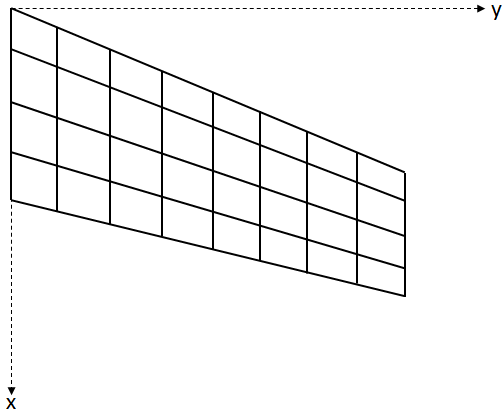
\includegraphics{DoubletLatticeWing.png}\hfill}

\end{fulllineitems}

\index{plotRigidWing() (AeroComBAT.AircraftParts.Wing method)}

\begin{fulllineitems}
\phantomsection\label{AircraftParts:AeroComBAT.AircraftParts.Wing.plotRigidWing}\pysiglinewithargsret{\bfcode{plotRigidWing}}{\emph{**kwargs}}{}
Plots the rigid wing.

This method plots the rigid model of the wing. This includes the
reference axis of the beams, the cross-sections of the beams, and the
lifting surfaces that make up the wing. This is an excellent check to
perform before adding the part to a FEM model.
\begin{quote}\begin{description}
\item[{Args}] \leavevmode
\end{description}\end{quote}
\begin{itemize}
\item {} \begin{description}
\item[{\emph{figName (str)}: The name of the MayaVi figure. `Rigid Wing' by}] \leavevmode
default.

\end{description}

\item {} \begin{description}
\item[{\emph{numXSects (int)}: The number of cross-sections that each wing}] \leavevmode
section will display. By default it is 2.

\end{description}

\item {} \begin{description}
\item[{\emph{color (1x3 tuple(int))}: This is a length 3 tuple to be used as the}] \leavevmode
color of the beam reference axes. Black by default.

\end{description}

\end{itemize}
\begin{quote}\begin{description}
\item[{Returns}] \leavevmode
\end{description}\end{quote}
\begin{itemize}
\item {} 
None

\end{itemize}

\end{fulllineitems}


\end{fulllineitems}



\section{Structures Module}
\label{structures::doc}\label{structures:structures-module}\label{structures:module-AeroComBAT.Structures}\index{AeroComBAT.Structures (module)}
This module contains a library of classes devoted to structural analysis.

The primary purpose of this library is to fascilitate the ROM (reduced order
modeling) of structures that can simplified to beams. The real power of this
library comes from it's the XSect class. This class can create and analyze
a cross-section, allowing the user to accurately model a nonhomogeneous
(made of multiple materials) anisotropic (materials that behave anisotropically
such as composites) complex cross-sections.

It should be noted that classes are ordered by model complexity. The further
down the structures.py library, the more complex the objects, often requiring
multiple of their predecessors. For example, the CQUADX class requires four
node objects and a material object.
\begin{quote}\begin{description}
\item[{SUMARRY OF THE CLASSES}] \leavevmode
\end{description}\end{quote}
\begin{itemize}
\item {} 
\emph{Node}: Creates a node object with 3D position.

\item {} 
\emph{Material}: Creates a material object, generating the 3D constitutive relations.

\item {} \begin{description}
\item[{\emph{MicroMechanics}: Class to fascilitate the calculation of composite stiffnesses}] \leavevmode
using micro-mechanical models where fibers are long and continuous.

\end{description}

\item {} \begin{description}
\item[{\emph{CQUADX}: Creates a 2D linear quadrilateral element, mainly used to fascilitate    cross-sectional analysis, this class could be modified in future updates}] \leavevmode
such that they could also be used to create plate or laminate element
objects as well.

\end{description}

\item {} \begin{description}
\item[{\emph{MaterialLib}: Creates a material library object meant to hold many material}] \leavevmode
objects.

\end{description}

\item {} 
\emph{Ply}: Creates ply objects which are used in the building of a laminate object.

\item {} \begin{description}
\item[{\emph{Laminate}: Creates laminate objects which could be used for CLT (classical}] \leavevmode
lamination theory) analysis as well as to be used in building a beam
cross-section.

\end{description}

\item {} \begin{description}
\item[{\emph{XSect}: Creates a cross-section object which can be used in the ROM of a beam}] \leavevmode
with a non-homogeneous anisotropic cross-section. Currently only supports
simple box beam cross-section (i.e., four laminates joined together to form
a box), however outer mold lines can take the shape of airfoil profiles.
See the Airfoil class in AircraftParts.py for more info.

\end{description}

\item {} 
\emph{TBeam}: Creates a single Timoshenko beam object for FEA.

\item {} \begin{description}
\item[{\emph{SuperBeam}: Creates a super beam object. This class is mainly used to automate}] \leavevmode
the creation of many connected TBeam objects to be used late for FEA.

\end{description}

\item {} \begin{description}
\item[{\emph{WingSection}: A class which creates and holds many super beams, each of which}] \leavevmode
could have different cross-sections. It also helps to dimensionalize
plates for simple closed-form composite buckling load aproximations.

\end{description}

\end{itemize}

\begin{notice}{note}{Note:}
Currently the inclusion of thermal strains are not supported for any
structural model.
\end{notice}


\subsection{NODE}
\label{structures:node}\index{Node (class in AeroComBAT.Structures)}

\begin{fulllineitems}
\phantomsection\label{structures:AeroComBAT.Structures.Node}\pysiglinewithargsret{\strong{class }\code{AeroComBAT.Structures.}\bfcode{Node}}{\emph{NID}, \emph{x}}{}
Creates a node object.

Node objects could be used in any finite element implementation.
\begin{quote}\begin{description}
\item[{Attributes}] \leavevmode
\end{description}\end{quote}
\begin{itemize}
\item {} 
\emph{NID (int)}: The integer identifier given to the object.

\item {} \begin{description}
\item[{\emph{x (Array{[}float{]})}: An array containing the 3 x-y-z coordinates of the}] \leavevmode
node.

\end{description}

\item {} \begin{description}
\item[{\emph{summary (str)}: A string which is a tabulated respresentation and}] \leavevmode
summary of the important attributes of the object.

\end{description}

\end{itemize}
\begin{quote}\begin{description}
\item[{Methods}] \leavevmode
\end{description}\end{quote}
\begin{itemize}
\item {} \begin{description}
\item[{\emph{printSummary}: This method prints out basic information about the node}] \leavevmode
object, such as it's node ID and it's x-y-z coordinates

\end{description}

\end{itemize}
\index{\_\_init\_\_() (AeroComBAT.Structures.Node method)}

\begin{fulllineitems}
\phantomsection\label{structures:AeroComBAT.Structures.Node.__init__}\pysiglinewithargsret{\bfcode{\_\_init\_\_}}{\emph{NID}, \emph{x}}{}
Initializes the node object.
\begin{quote}\begin{description}
\item[{Args}] \leavevmode
\end{description}\end{quote}
\begin{itemize}
\item {} 
\emph{nid (int)}: The desired integer node ID

\item {} 
\emph{x (Array{[}float{]})}: The position of the node in 3D space.

\end{itemize}
\begin{quote}\begin{description}
\item[{Returns}] \leavevmode
\end{description}\end{quote}
\begin{itemize}
\item {} 
None

\end{itemize}

\end{fulllineitems}

\index{printSummary() (AeroComBAT.Structures.Node method)}

\begin{fulllineitems}
\phantomsection\label{structures:AeroComBAT.Structures.Node.printSummary}\pysiglinewithargsret{\bfcode{printSummary}}{}{}
Prints basic information about the node.

The printSummary method prints out basic node attributes in an organized
fashion. This includes the node ID and x-y-z global coordinates.
\begin{quote}\begin{description}
\item[{Args}] \leavevmode
\end{description}\end{quote}
\begin{itemize}
\item {} 
None

\end{itemize}
\begin{quote}\begin{description}
\item[{Returns}] \leavevmode
\end{description}\end{quote}
\begin{itemize}
\item {} 
A printed table including the node ID and it's coordinates

\end{itemize}

\end{fulllineitems}


\end{fulllineitems}



\subsection{MATERIAL}
\label{structures:material}\index{Material (class in AeroComBAT.Structures)}

\begin{fulllineitems}
\phantomsection\label{structures:AeroComBAT.Structures.Material}\pysiglinewithargsret{\strong{class }\code{AeroComBAT.Structures.}\bfcode{Material}}{\emph{MID}, \emph{name}, \emph{matType}, \emph{mat\_constants}, \emph{mat\_t}, \emph{**kwargs}}{}
creates a linear elastic material object.

This class creates a material object which can be stored within a
material library object. The material can be in general orthotropic.
\begin{quote}\begin{description}
\item[{Attributes}] \leavevmode
\end{description}\end{quote}
\begin{itemize}
\item {} 
\emph{name (str)}: A name for the material.

\item {} 
\emph{MID (int)}: An integer identifier for the material.

\item {} \begin{description}
\item[{\emph{matType (str)}: A string expressing what type of material it is.}] \leavevmode
Currently, the supported materials are isotropic, transversely
isotropic, and orthotropic.

\end{description}

\item {} \begin{description}
\item[{\emph{summary (str)}: A string which is a tabulated respresentation and}] \leavevmode
summary of the important attributes of the object.

\end{description}

\item {} \begin{description}
\item[{\emph{t (float)}: A single float which represents the thickness of a ply if}] \leavevmode
the material is to be used in a composite.

\end{description}

\item {} \begin{description}
\item[{\emph{rho (float)}: A single float which represents the density of the}] \leavevmode
materials.

\end{description}

\item {} \begin{description}
\item[{\emph{Smat (6x6 numpy Array{[}float{]})}: A numpy array representing the}] \leavevmode
compliance matrix in the fiber coordinate system.*

\end{description}

\item {} \begin{description}
\item[{\emph{Cmat (6x6 numpy Array{[}float{]})}: A numpy array representing the}] \leavevmode
stiffness matrix in the fiber coordinate system.*

\end{description}

\end{itemize}
\begin{quote}\begin{description}
\item[{Methods}] \leavevmode
\end{description}\end{quote}
\begin{itemize}
\item {} \begin{description}
\item[{\emph{printSummary}: This method prints out basic information about the}] \leavevmode
material, including the type, the material constants, material
thickness, as well as the tabulated stiffness or compliance
matricies if requested.

\end{description}

\end{itemize}

\begin{notice}{note}{Note:}
The CQUADX element assumes that the fibers are oriented along
the (1,0,0) in the global coordinate system.
\end{notice}
\index{\_\_init\_\_() (AeroComBAT.Structures.Material method)}

\begin{fulllineitems}
\phantomsection\label{structures:AeroComBAT.Structures.Material.__init__}\pysiglinewithargsret{\bfcode{\_\_init\_\_}}{\emph{MID}, \emph{name}, \emph{matType}, \emph{mat\_constants}, \emph{mat\_t}, \emph{**kwargs}}{}
Creates a material object

The main purpose of this class is assembling the constitutive
relations. Regardless of the analysis
\begin{quote}\begin{description}
\item[{Args}] \leavevmode
\end{description}\end{quote}
\begin{itemize}
\item {} 
\emph{MID (int)}: Material ID.

\item {} 
\emph{name (str)}: Name of the material.

\item {} \begin{description}
\item[{\emph{matType (str)}: The type of the material. Supported material types}] \leavevmode
are ``iso'', ``trans\_iso'', and ``ortho''.

\end{description}

\item {} \begin{description}
\item[{\emph{mat\_constants (1xX Array{[}Float{]})}: The requisite number of material}] \leavevmode
constants required for any structural analysis. Note, this
array includes the material density. For example, an isotropic
material needs 2 elastic material constants, so the total
length of mat\_constants would be 3, 2 elastic constants and the
density.

\end{description}

\item {} 
\emph{mat\_t (float)}: The thickness of 1-ply of the material

\item {} \begin{description}
\item[{\emph{th (1x3 Array{[}float{]})}: The angles about which the material can be}] \leavevmode
rotated when it is initialized. In degrees.

\end{description}

\end{itemize}
\begin{quote}\begin{description}
\item[{Returns}] \leavevmode
\end{description}\end{quote}
\begin{itemize}
\item {} 
None

\end{itemize}

\begin{notice}{note}{Note:}
While this class supports material direction rotations, it is more
robust to simply let the CQUADX and Mesher class handle all material
rotations.
\end{notice}

\end{fulllineitems}

\index{printSummary() (AeroComBAT.Structures.Material method)}

\begin{fulllineitems}
\phantomsection\label{structures:AeroComBAT.Structures.Material.printSummary}\pysiglinewithargsret{\bfcode{printSummary}}{\emph{**kwargs}}{}
Prints a tabulated summary of the material.

This method prints out basic information about the
material, including the type, the material constants, material
thickness, as well as the tabulated stiffness or compliance
matricies if requested.
\begin{quote}\begin{description}
\item[{Args}] \leavevmode
\end{description}\end{quote}
\begin{itemize}
\item {} \begin{description}
\item[{\emph{compliance (str)}: A boolean input to signify if the compliance}] \leavevmode
matrix should be printed.

\end{description}

\item {} \begin{description}
\item[{\emph{stiffness (str)}: A boolean input to signify if the stiffness matrix}] \leavevmode
should be printed.

\end{description}

\end{itemize}
\begin{quote}\begin{description}
\item[{Returns}] \leavevmode
\end{description}\end{quote}
\begin{itemize}
\item {} \begin{description}
\item[{String print out containing the material name, as well as material}] \leavevmode
constants and other defining material attributes. If requested
this includes the material stiffness and compliance matricies.

\end{description}

\end{itemize}

\end{fulllineitems}


\end{fulllineitems}



\subsection{CQUADX}
\label{structures:cquadx}\index{CQUADX (class in AeroComBAT.Structures)}

\begin{fulllineitems}
\phantomsection\label{structures:AeroComBAT.Structures.CQUADX}\pysiglinewithargsret{\strong{class }\code{AeroComBAT.Structures.}\bfcode{CQUADX}}{\emph{EID}, \emph{nodes}, \emph{MID}, \emph{matLib}, \emph{**kwargs}}{}
Creates a linear, 2D 4 node quadrilateral element object.

The main purpose of this class is to assist in the cross-sectional
analysis of a beam, however it COULD be modified to serve as an element for
2D plate or laminate FE analysis.
\begin{quote}\begin{description}
\item[{Attributes}] \leavevmode
\end{description}\end{quote}
\begin{itemize}
\item {} 
\emph{type (str)}: A string designating it a CQUADX element.

\item {} \begin{description}
\item[{\emph{xsect (bool)}: States whether the element is to be used in cross-}] \leavevmode
sectional analysis.

\end{description}

\item {} \begin{description}
\item[{\emph{th (1x3 Array{[}float{]})}: Array containing the Euler-angles expressing how}] \leavevmode
the element constitutive relations should be rotated from the
material fiber frame to the global CSYS. In degrees.

\end{description}

\item {} 
\emph{EID (int)}: An integer identifier for the CQUADX element.

\item {} \begin{description}
\item[{\emph{MID (int)}: An integer refrencing the material ID used for the}] \leavevmode
constitutive relations.

\end{description}

\item {} \begin{description}
\item[{\emph{NIDs (1x4 Array{[}int{]})}: Contains the integer node identifiers for the}] \leavevmode
node objects used to create the element.

\end{description}

\item {} \begin{description}
\item[{\emph{nodes (1x4 Array{[}obj{]})}: Contains the properly ordered nodes objects}] \leavevmode
used to create the element.

\end{description}

\item {} \begin{description}
\item[{\emph{xs (1x4 np.array{[}float{]})}: Array containing the x-coordinates of the}] \leavevmode
nodes used in the element

\end{description}

\item {} \begin{description}
\item[{\emph{ys (1x4 np.array{[}float{]})}: Array containing the y-coordinates of the}] \leavevmode
nodes used in the element

\end{description}

\item {} 
\emph{rho (float)}: Density of the material used in the element.

\item {} 
\emph{mass (float)}: Mass per unit length (or thickness) of the element.

\item {} \begin{description}
\item[{\emph{U (12x1 np.array{[}float{]})}: This column vector contains the CQUADXs}] \leavevmode
3 DOF (x-y-z) displacements in the local xsect CSYS due to cross-
section warping effects.

\end{description}

\item {} \begin{description}
\item[{\emph{Eps (6x4 np.array{[}float{]})}: A matrix containing the 3D strain state}] \leavevmode
within the CQUADX element.

\end{description}

\item {} \begin{description}
\item[{\emph{Sig (6x4 np.array{[}float{]})}: A matrix containing the 3D stress state}] \leavevmode
within the CQUADX element.

\end{description}

\end{itemize}
\begin{quote}\begin{description}
\item[{Methods}] \leavevmode
\end{description}\end{quote}
\begin{itemize}
\item {} \begin{description}
\item[{\emph{x}: Calculates the local xsect x-coordinate provided the desired master}] \leavevmode
coordinates eta and xi.

\end{description}

\item {} \begin{description}
\item[{\emph{y}: Calculates the local xsect y-coordinate provided the desired master}] \leavevmode
coordinates eta and xi.

\end{description}

\item {} \begin{description}
\item[{\emph{J}: Calculates the jacobian of the element provided the desired master}] \leavevmode
coordinates eta and xi.

\end{description}

\item {} \begin{description}
\item[{\emph{resetResults}: Initializes the displacement (U), strain (Eps), and}] \leavevmode
stress (Sig) attributes of the element.

\end{description}

\item {} \begin{description}
\item[{\emph{getDeformed}: Provided an analysis has been conducted, this method}] \leavevmode
returns 3 2x2 np.array{[}float{]} containing the element warped
displacements in the local xsect CSYS.

\end{description}

\item {} \begin{description}
\item[{\emph{getStressState}: Provided an analysis has been conducted, this method}] \leavevmode
returns 3 2x2 np.array{[}float{]} containing the element stress at four
points. The 3D stress state is processed to return the Von-Mises
or Maximum Principal stress state.

\end{description}

\item {} \begin{description}
\item[{\emph{printSummary}: Prints out a tabulated form of the element ID, as well}] \leavevmode
as the node ID's referenced by the element.

\end{description}

\end{itemize}
\index{J() (AeroComBAT.Structures.CQUADX method)}

\begin{fulllineitems}
\phantomsection\label{structures:AeroComBAT.Structures.CQUADX.J}\pysiglinewithargsret{\bfcode{J}}{\emph{eta}, \emph{xi}}{}
Calculates the jacobian at a point in the element.

This method calculates the jacobian at a local point within the element
provided the master coordinates eta and xi.
\begin{quote}\begin{description}
\item[{Args}] \leavevmode
\end{description}\end{quote}
\begin{itemize}
\item {} 
\emph{eta (float)}: The eta coordinate in the master coordinate domain.*

\item {} 
\emph{xi (float)}: The xi coordinate in the master coordinate domain.*

\end{itemize}
\begin{quote}\begin{description}
\item[{Returns}] \leavevmode
\end{description}\end{quote}
\begin{itemize}
\item {} \begin{description}
\item[{\emph{Jmat (3x3 np.array{[}float{]})}: The stress-resutlant transformation}] \leavevmode
array.

\end{description}

\end{itemize}

\begin{notice}{note}{Note:}
Xi and eta can both vary between -1 and 1 respectively.
\end{notice}

\end{fulllineitems}

\index{\_\_init\_\_() (AeroComBAT.Structures.CQUADX method)}

\begin{fulllineitems}
\phantomsection\label{structures:AeroComBAT.Structures.CQUADX.__init__}\pysiglinewithargsret{\bfcode{\_\_init\_\_}}{\emph{EID}, \emph{nodes}, \emph{MID}, \emph{matLib}, \emph{**kwargs}}{}
Initializes the element.
\begin{quote}\begin{description}
\item[{Args}] \leavevmode
\end{description}\end{quote}
\begin{itemize}
\item {} 
\emph{EID (int)}: An integer identifier for the CQUADX element.

\item {} \begin{description}
\item[{\emph{nodes (1x4 Array{[}obj{]})}: Contains the properly ordered nodes objects}] \leavevmode
used to create the element.

\end{description}

\item {} \begin{description}
\item[{\emph{MID (int)}: An integer refrencing the material ID used for the}] \leavevmode
constitutive relations.

\end{description}

\item {} \begin{description}
\item[{\emph{matLib (obj)}: A material library object containing a dictionary}] \leavevmode
with the material corresponding to the provided MID.

\end{description}

\item {} \begin{description}
\item[{\emph{xsect (bool)}: A boolean to determine whether this quad element is}] \leavevmode
to be used for cross-sectional analysis. Defualt value is True.

\end{description}

\item {} \begin{description}
\item[{\emph{th (1x3 Array{[}float{]})}: Array containing the Euler-angles expressing}] \leavevmode
how the element constitutive relations should be rotated from
the material fiber frame to the global CSYS. In degrees.

\end{description}

\end{itemize}
\begin{quote}\begin{description}
\item[{Returns}] \leavevmode
\end{description}\end{quote}
\begin{itemize}
\item {} 
None

\end{itemize}

\begin{notice}{note}{Note:}
The reference coordinate system for cross-sectional analysis is a
\end{notice}

local coordinate system in which the x and y axes are planer with the
element, and the z-axis is perpendicular to the plane of the element.

\end{fulllineitems}

\index{getDeformed() (AeroComBAT.Structures.CQUADX method)}

\begin{fulllineitems}
\phantomsection\label{structures:AeroComBAT.Structures.CQUADX.getDeformed}\pysiglinewithargsret{\bfcode{getDeformed}}{\emph{**kwargs}}{}
Returns the warping displacement of the element.

Provided an analysis has been conducted, this method
returns 3 2x2 np.array{[}float{]} containing the element warped
displacements in the local xsect CSYS.
\begin{quote}\begin{description}
\item[{Args}] \leavevmode
\end{description}\end{quote}
\begin{itemize}
\item {} \begin{description}
\item[{\emph{warpScale (float)}: A multiplicative scaling factor intended to}] \leavevmode
exagerate the warping displacement within the cross-section.

\end{description}

\end{itemize}
\begin{quote}\begin{description}
\item[{Returns}] \leavevmode
\end{description}\end{quote}
\begin{itemize}
\item {} \begin{description}
\item[{\emph{xdef (2x2 np.array{[}float{]})}: warped x-coordinates at the four corner}] \leavevmode
points.

\end{description}

\item {} \begin{description}
\item[{\emph{ydef (2x2 np.array{[}float{]})}: warped y-coordinates at the four corner}] \leavevmode
points.

\end{description}

\item {} \begin{description}
\item[{\emph{zdef (2x2 np.array{[}float{]})}: warped z-coordinates at the four corner}] \leavevmode
points.

\end{description}

\end{itemize}

\end{fulllineitems}

\index{getStressState() (AeroComBAT.Structures.CQUADX method)}

\begin{fulllineitems}
\phantomsection\label{structures:AeroComBAT.Structures.CQUADX.getStressState}\pysiglinewithargsret{\bfcode{getStressState}}{\emph{crit='VonMis'}}{}
Returns the stress state of the element.

Provided an analysis has been conducted, this method
returns a 2x2 np.array{[}float{]} containing the element the 3D stress
state at the four guass points by default.*
\begin{quote}\begin{description}
\item[{Args}] \leavevmode
\end{description}\end{quote}
\begin{itemize}
\item {} \begin{description}
\item[{\emph{crit (str)}: Determines what criteria is used to evaluate the 3D}] \leavevmode
stress state at the sample points within the element. By
default the Von Mises stress is returned. Currently supported
options include: Von Mises (`VonMis'), maximum principle stress
(`MaxPrin'), the minimum principle stress (`MinPrin'), and the
local cross-section stress states `sig\_xx' where the subindeces can
go from 1-3. The keyword `none' is also an option.

\end{description}

\end{itemize}
\begin{quote}\begin{description}
\item[{Returns}] \leavevmode
\end{description}\end{quote}
\begin{itemize}
\item {} \begin{description}
\item[{\emph{sigData (2x2 np.array{[}float{]})}: The stress state evaluated at four}] \leavevmode
points within the CQUADX element.

\end{description}

\end{itemize}

\begin{notice}{note}{Note:}
The XSect method calcWarpEffects is what determines where strain
\end{notice}

and stresses are sampled. By default it samples this information at the
Guass points where the stress/strain will be most accurate.

\end{fulllineitems}

\index{printSummary() (AeroComBAT.Structures.CQUADX method)}

\begin{fulllineitems}
\phantomsection\label{structures:AeroComBAT.Structures.CQUADX.printSummary}\pysiglinewithargsret{\bfcode{printSummary}}{\emph{nodes=False}}{}
A method for printing a summary of the CQUADX element.

Prints out a tabulated form of the element ID, as well as the node ID's
referenced by the element.
\begin{quote}\begin{description}
\item[{Args}] \leavevmode
\end{description}\end{quote}
\begin{itemize}
\item {} 
None

\end{itemize}
\begin{quote}\begin{description}
\item[{Returns}] \leavevmode
\end{description}\end{quote}
\begin{itemize}
\item {} \begin{description}
\item[{\emph{summary (str)}: Prints the tabulated EID, node IDs and material IDs}] \leavevmode
associated with the CQUADX element.

\end{description}

\end{itemize}

\end{fulllineitems}

\index{resetResults() (AeroComBAT.Structures.CQUADX method)}

\begin{fulllineitems}
\phantomsection\label{structures:AeroComBAT.Structures.CQUADX.resetResults}\pysiglinewithargsret{\bfcode{resetResults}}{}{}
Resets stress, strain and warping displacement results.

Method is mainly intended to prevent results for one analysis or
sampling location in the matrix to effect the results in another.
\begin{quote}\begin{description}
\item[{Args}] \leavevmode
\end{description}\end{quote}
\begin{itemize}
\item {} 
None

\end{itemize}
\begin{quote}\begin{description}
\item[{Returns}] \leavevmode
\end{description}\end{quote}
\begin{itemize}
\item {} 
None

\end{itemize}

\end{fulllineitems}

\index{x() (AeroComBAT.Structures.CQUADX method)}

\begin{fulllineitems}
\phantomsection\label{structures:AeroComBAT.Structures.CQUADX.x}\pysiglinewithargsret{\bfcode{x}}{\emph{eta}, \emph{xi}}{}
Calculate the x-coordinate within the element.

Calculates the local xsect x-coordinate provided the desired master
coordinates eta and xi.
\begin{quote}\begin{description}
\item[{Args}] \leavevmode
\end{description}\end{quote}
\begin{itemize}
\item {} 
\emph{eta (float)}: The eta coordinate in the master coordinate domain.*

\item {} 
\emph{xi (float)}: The xi coordinate in the master coordinate domain.*

\end{itemize}
\begin{quote}\begin{description}
\item[{Returns}] \leavevmode
\end{description}\end{quote}
\begin{itemize}
\item {} 
\emph{x (float)}: The x-coordinate within the element.

\end{itemize}

\begin{notice}{note}{Note:}
Xi and eta can both vary between -1 and 1 respectively.
\end{notice}

\end{fulllineitems}

\index{y() (AeroComBAT.Structures.CQUADX method)}

\begin{fulllineitems}
\phantomsection\label{structures:AeroComBAT.Structures.CQUADX.y}\pysiglinewithargsret{\bfcode{y}}{\emph{eta}, \emph{xi}}{}
Calculate the y-coordinate within the element.

Calculates the local xsect y-coordinate provided the desired master
coordinates eta and xi.
\begin{quote}\begin{description}
\item[{Args}] \leavevmode
\end{description}\end{quote}
\begin{itemize}
\item {} 
\emph{eta (float)}: The eta coordinate in the master coordinate domain.*

\item {} 
\emph{xi (float)}: The xi coordinate in the master coordinate domain.*

\end{itemize}
\begin{quote}\begin{description}
\item[{Returns}] \leavevmode
\end{description}\end{quote}
\begin{itemize}
\item {} 
{\color{red}\bfseries{}{}`}y (float)': The y-coordinate within the element.

\end{itemize}

\begin{notice}{note}{Note:}
Xi and eta can both vary between -1 and 1 respectively.
\end{notice}

\end{fulllineitems}


\end{fulllineitems}



\subsection{MATERIAL LIBRARY}
\label{structures:material-library}\index{MaterialLib (class in AeroComBAT.Structures)}

\begin{fulllineitems}
\phantomsection\label{structures:AeroComBAT.Structures.MaterialLib}\pysigline{\strong{class }\code{AeroComBAT.Structures.}\bfcode{MaterialLib}}
Creates a material library object.

This material library holds the materials to be used for any type of
analysis. Furthermore, it can be used to generate new material objects
to be automatically stored within it. See the Material class for suported
material types.
\begin{quote}\begin{description}
\item[{Attributes}] \leavevmode
\end{description}\end{quote}
\begin{itemize}
\item {} \begin{description}
\item[{\emph{matDict (dict)}: A dictionary which stores material objects as the}] \leavevmode
values with the MIDs as the associated keys.

\end{description}

\end{itemize}
\begin{quote}\begin{description}
\item[{Methods}] \leavevmode
\end{description}\end{quote}
\begin{itemize}
\item {} 
\emph{addMat}: Adds a material to the MaterialLib object dictionary.

\item {} 
\emph{getMat}: Returns a material object provided an MID

\item {} \begin{description}
\item[{\emph{printSummary}: Prints a summary of all of the materials held within the}] \leavevmode
matDict dictionary.

\end{description}

\end{itemize}
\index{\_\_init\_\_() (AeroComBAT.Structures.MaterialLib method)}

\begin{fulllineitems}
\phantomsection\label{structures:AeroComBAT.Structures.MaterialLib.__init__}\pysiglinewithargsret{\bfcode{\_\_init\_\_}}{}{}
Initialize MaterialLib object.

The initialization method is mainly used to initialize a dictionary
which houses material objects.
\begin{quote}\begin{description}
\item[{Args}] \leavevmode
\end{description}\end{quote}
\begin{itemize}
\item {} 
None

\end{itemize}
\begin{quote}\begin{description}
\item[{Returns}] \leavevmode
\end{description}\end{quote}
\begin{itemize}
\item {} 
None

\end{itemize}

\end{fulllineitems}

\index{addMat() (AeroComBAT.Structures.MaterialLib method)}

\begin{fulllineitems}
\phantomsection\label{structures:AeroComBAT.Structures.MaterialLib.addMat}\pysiglinewithargsret{\bfcode{addMat}}{\emph{MID}, \emph{mat\_name}, \emph{mat\_type}, \emph{mat\_constants}, \emph{mat\_t}, \emph{**kwargs}}{}
Add a material to the MaterialLib object.

This is the primary method of the class, used to create new material
obects and then add them to the library for later use.
\begin{quote}\begin{description}
\item[{Args}] \leavevmode
\end{description}\end{quote}
\begin{itemize}
\item {} 
\emph{MID (int)}: Material ID.

\item {} 
\emph{name (str)}: Name of the material.

\item {} \begin{description}
\item[{\emph{matType (str)}: The type of the material. Supported material types}] \leavevmode
are ``iso'', ``trans\_iso'', and ``ortho''.

\end{description}

\item {} \begin{description}
\item[{\emph{mat\_constants (1xX Array{[}Float{]})}: The requisite number of material}] \leavevmode
constants required for any structural analysis. Note, this
array includes the material density. For example, an isotropic
material needs 2 elastic material constants, so the total
length of mat\_constants would be 3, 2 elastic constants and the
density.

\end{description}

\item {} 
\emph{mat\_t (float)}: The thickness of 1-ply of the material

\item {} \begin{description}
\item[{\emph{th (1x3 Array{[}float{]})}: The angles about which the material can be}] \leavevmode
rotated when it is initialized. In degrees.

\end{description}

\item {} \begin{description}
\item[{\emph{overwrite (bool)}: Input used in order to define whether the}] \leavevmode
material being added can overwrite another material already
held by the material library with the same MID.

\end{description}

\end{itemize}
\begin{quote}\begin{description}
\item[{Returns}] \leavevmode
\end{description}\end{quote}
\begin{itemize}
\item {} 
None

\end{itemize}

\end{fulllineitems}

\index{getMat() (AeroComBAT.Structures.MaterialLib method)}

\begin{fulllineitems}
\phantomsection\label{structures:AeroComBAT.Structures.MaterialLib.getMat}\pysiglinewithargsret{\bfcode{getMat}}{\emph{MID}}{}
Method that returns a material from the material libary
\begin{quote}\begin{description}
\item[{Args}] \leavevmode
\end{description}\end{quote}
\begin{itemize}
\item {} 
\emph{MID (int)}: The ID of the material which is desired

\end{itemize}
\begin{quote}\begin{description}
\item[{Returns}] \leavevmode
\end{description}\end{quote}
\begin{itemize}
\item {} 
{\color{red}\bfseries{}{}`}(obj): A material object associated with the key MID

\end{itemize}

\end{fulllineitems}

\index{printSummary() (AeroComBAT.Structures.MaterialLib method)}

\begin{fulllineitems}
\phantomsection\label{structures:AeroComBAT.Structures.MaterialLib.printSummary}\pysiglinewithargsret{\bfcode{printSummary}}{}{}
Prints summary of all Materials in MaterialLib

A method used to print out tabulated summary of all of the materials
held within the material library object.
\begin{quote}\begin{description}
\item[{Args}] \leavevmode
\end{description}\end{quote}
\begin{itemize}
\item {} 
None

\end{itemize}
\begin{quote}\begin{description}
\item[{Returns}] \leavevmode
\end{description}\end{quote}
\begin{itemize}
\item {} 
(str): A tabulated summary of the materials.

\end{itemize}

\end{fulllineitems}


\end{fulllineitems}



\subsection{PLY}
\label{structures:ply}\index{Ply (class in AeroComBAT.Structures)}

\begin{fulllineitems}
\phantomsection\label{structures:AeroComBAT.Structures.Ply}\pysiglinewithargsret{\strong{class }\code{AeroComBAT.Structures.}\bfcode{Ply}}{\emph{Material}, \emph{th}}{}
Creates a CLT ply object.

A class inspired by CLT, this class can be used to generate laminates
to be used for CLT or cross-sectional analysis. It is likely that ply
objects won't be created individually and then assembeled into a lamiante.
More likely is that the plies will be generated within the laminate object.
It should also be noted that it is assumed that the materials used are
effectively at most transversely isotropic.
\begin{quote}\begin{description}
\item[{Attributes}] \leavevmode
\end{description}\end{quote}
\begin{itemize}
\item {} 
\emph{E1 (float)}: Stiffness in the fiber direction.

\item {} 
\emph{E2 (float)}: Stiffness transverse to the fiber direction.

\item {} 
\emph{nu\_12 (float)}: In plane poisson ratio.

\item {} 
\emph{G\_12 (float)}: In plane shear modulus.

\item {} 
\emph{t (float)}: Thickness of the ply.

\item {} \begin{description}
\item[{\emph{Qbar (1x6 np.array{[}float{]})}: The terms in the rotated, reduced stiffness}] \leavevmode
matrix. Ordering is as follows: {[}Q11,Q12,Q16,Q22,Q26,Q66{]}

\end{description}

\item {} \begin{description}
\item[{\emph{MID (int)}: An integer refrencing the material ID used for the}] \leavevmode
constitutive relations.

\end{description}

\item {} \begin{description}
\item[{\emph{th (float)}: The angle about which the fibers are rotated in the plane}] \leavevmode
in degrees.

\end{description}

\end{itemize}
\begin{quote}\begin{description}
\item[{Methods}] \leavevmode
\end{description}\end{quote}
\begin{itemize}
\item {} \begin{description}
\item[{\emph{genQ}: Given the in-plane stiffnesses used by the material of the ply,}] \leavevmode
the method calculates the terms of ther reduced stiffness matrix.

\end{description}

\item {} \begin{description}
\item[{\emph{printSummary}: This prints out a summary of the object, including}] \leavevmode
thickness, referenced MID and in plane angle orientation theta in
degrees.

\end{description}

\end{itemize}
\index{\_\_init\_\_() (AeroComBAT.Structures.Ply method)}

\begin{fulllineitems}
\phantomsection\label{structures:AeroComBAT.Structures.Ply.__init__}\pysiglinewithargsret{\bfcode{\_\_init\_\_}}{\emph{Material}, \emph{th}}{}
Initializes the ply.

This method initializes information about the ply such as in-plane
stiffness repsonse.
\begin{quote}\begin{description}
\item[{Args}] \leavevmode
\end{description}\end{quote}
\begin{itemize}
\item {} \begin{description}
\item[{\emph{Material (obj)}: A material object, most likely coming from a}] \leavevmode
material library.

\end{description}

\item {} \begin{description}
\item[{\emph{th (float)}: The angle about which the fibers are rotated in the}] \leavevmode
plane in degrees.

\end{description}

\end{itemize}
\begin{quote}\begin{description}
\item[{Returns}] \leavevmode
\end{description}\end{quote}
\begin{itemize}
\item {} 
None

\end{itemize}

\end{fulllineitems}

\index{genQ() (AeroComBAT.Structures.Ply method)}

\begin{fulllineitems}
\phantomsection\label{structures:AeroComBAT.Structures.Ply.genQ}\pysiglinewithargsret{\bfcode{genQ}}{\emph{E1}, \emph{E2}, \emph{nu12}, \emph{G12}}{}
A method for calculating the reduced compliance of the ply.

Intended primarily as a private method but left public, this method,
for those unfarmiliar with CLT, calculates the terms in the reduced stiffness
matrix given the in plane ply stiffnesses. It can be thus inferred that
this requires the assumption of plane stres. This method is primarily
used during the ply instantiation.
\begin{quote}\begin{description}
\item[{Args}] \leavevmode
\end{description}\end{quote}
\begin{itemize}
\item {} 
\emph{E1 (float)}: The fiber direction stiffness.

\item {} 
\emph{E2 (float)}: The stiffness transverse to the fibers.

\item {} 
\emph{nu12 (float)}: The in-plane poisson ratio.

\item {} 
\emph{G12 (float)}: The in-plane shear stiffness.

\end{itemize}
\begin{quote}\begin{description}
\item[{Returns}] \leavevmode
\end{description}\end{quote}
\begin{itemize}
\item {} \begin{description}
\item[{\emph{(1x4 np.array{[}float{]})}: The terms used in the reduced stiffness}] \leavevmode
matrix. The ordering is: {[}Q11,Q12,Q22,Q66{]}.

\end{description}

\end{itemize}

\end{fulllineitems}

\index{printSummary() (AeroComBAT.Structures.Ply method)}

\begin{fulllineitems}
\phantomsection\label{structures:AeroComBAT.Structures.Ply.printSummary}\pysiglinewithargsret{\bfcode{printSummary}}{}{}
Prints a summary of the ply object.

A method for printing a summary of the ply properties, such as
the material ID, fiber orientation and ply thickness.
\begin{quote}\begin{description}
\item[{Args}] \leavevmode
\end{description}\end{quote}
\begin{itemize}
\item {} 
None

\end{itemize}
\begin{quote}\begin{description}
\item[{Returns}] \leavevmode
\end{description}\end{quote}
\begin{itemize}
\item {} 
\emph{(str)}: Printed tabulated summary of the ply.

\end{itemize}

\end{fulllineitems}


\end{fulllineitems}



\subsection{LAMINATE}
\label{structures:laminate}\index{Laminate (class in AeroComBAT.Structures)}

\begin{fulllineitems}
\phantomsection\label{structures:AeroComBAT.Structures.Laminate}\pysiglinewithargsret{\strong{class }\code{AeroComBAT.Structures.}\bfcode{Laminate}}{\emph{n\_i\_tmp}, \emph{m\_i\_tmp}, \emph{matLib}, \emph{**kwargs}}{}
Creates a CLT laminate object.

This class has two main uses. It can either be used for CLT analysis, or it
can be used to build up a 2D mesh for a descretized cross-section.
\begin{quote}\begin{description}
\item[{Attributes}] \leavevmode
\end{description}\end{quote}
\begin{itemize}
\item {} \begin{description}
\item[{\emph{mesh (NxM np.array{[}int{]})}: This 2D array holds NIDs and is used}] \leavevmode
to represent how nodes are organized in the 2D cross-section of
the laminate.

\end{description}

\item {} \begin{description}
\item[{\emph{xmesh (NxM np.array{[}int{]})}: This 2D array holds the rigid x-coordinates}] \leavevmode
of the nodes within the 2D descretization of the laminate on the
local xsect CSYS.

\end{description}

\item {} \begin{description}
\item[{\emph{ymesh (NxM np.array{[}int{]})}: This 2D array holds the rigid y-coordinates}] \leavevmode
of the nodes within the 2D descretization of the laminate on the
local xsect CSYS.

\end{description}

\item {} \begin{description}
\item[{\emph{zmesh (NxM np.array{[}int{]})}: This 2D array holds the rigid z-coordinates}] \leavevmode
of the nodes within the 2D descretization of the laminate on the
local xsect CSYS.

\end{description}

\item {} 
\emph{H (float)}: The total laminate thickness.

\item {} 
\emph{rho\_A (float)}: The laminate area density.

\item {} \begin{description}
\item[{\emph{plies (1xN array{[}obj{]})}: Contains an array of ply objects used to}] \leavevmode
construct the laminate.

\end{description}

\item {} 
\emph{t (1xN array{[}float{]})}: An array containing all of the ply thicknesses.

\item {} \begin{description}
\item[{\emph{ABD (6x6 np.array{[}float{]})}: The CLT 6x6 matrix relating in-plane strains}] \leavevmode
and curvatures to in-plane force and moment resultants.

\end{description}

\item {} \begin{description}
\item[{\emph{abd (6x6 np.array{[}float{]})}: The CLT 6x6 matrix relating in-plane forces}] \leavevmode
and moments resultants to in-plane strains and curvatures.

\end{description}

\item {} \begin{description}
\item[{\emph{z (1xN array{[}float{]})}: The z locations of laminate starting and ending}] \leavevmode
points. This system always starts at -H/2 and goes to H/2

\end{description}

\item {} \begin{description}
\item[{\emph{equivMat (obj)}: This is orthotropic material object which exhibits}] \leavevmode
similar in-plane stiffnesses.

\end{description}

\item {} \begin{description}
\item[{\emph{forceRes (1x6 np.array{[}float{]})}: The applied or resulting force and}] \leavevmode
moment resultants generated during CLT analysis.

\end{description}

\item {} \begin{description}
\item[{\emph{globalStrain (1x6 np.array{[}float{]})}:  The applied or resulting strain}] \leavevmode
and curvatures generated during CLT analysis.

\end{description}

\end{itemize}
\begin{quote}\begin{description}
\item[{Methods}] \leavevmode
\end{description}\end{quote}
\begin{itemize}
\item {} \begin{description}
\item[{\emph{printSummary}: This method prints out defining attributes of the}] \leavevmode
laminate, such as the ABD matrix and layup schedule.

\end{description}

\end{itemize}
\index{\_\_init\_\_() (AeroComBAT.Structures.Laminate method)}

\begin{fulllineitems}
\phantomsection\label{structures:AeroComBAT.Structures.Laminate.__init__}\pysiglinewithargsret{\bfcode{\_\_init\_\_}}{\emph{n\_i\_tmp}, \emph{m\_i\_tmp}, \emph{matLib}, \emph{**kwargs}}{}
Initializes the Laminate object

The way the laminate initialization works is you pass in two-three
arrays and a material library. The first array contains information
about how many plies you want to stack, the second array determines
what material should be used for those plies, and the third array
determines at what angle those plies lie. The class was developed this
way as a means to fascilitate laminate optimization by quickly changing
the number of plies at a given orientation and using a given material.
\begin{quote}\begin{description}
\item[{Args}] \leavevmode
\end{description}\end{quote}
\begin{itemize}
\item {} \begin{description}
\item[{\emph{n\_i\_tmp (1xN array{[}int{]})}: An array containing the number of plies}] \leavevmode
using a material at a particular orientation such as:
(theta=0,theta=45...)

\end{description}

\item {} \begin{description}
\item[{\emph{m\_i\_tmp (1xN array{[}int{]})}: An array containing the material to be}] \leavevmode
used for the corresponding number of plies in the n\_i\_tmp array

\end{description}

\item {} \begin{description}
\item[{\emph{matLib (obj)}: The material library holding different material}] \leavevmode
objects.

\end{description}

\item {} 
\emph{sym (bool)}: Whether the laminate is symetric. (False by default)

\item {} \begin{description}
\item[{\emph{th (1xN array{[}float{]})}: An array containing the orientation at which}] \leavevmode
the fibers are positioned within the laminate.

\end{description}

\end{itemize}
\begin{quote}\begin{description}
\item[{Returns}] \leavevmode
\end{description}\end{quote}
\begin{itemize}
\item {} 
None

\end{itemize}

\begin{notice}{note}{Note:}
If you wanted to create a {[}0\_2/45\_2/90\_2/-45\_2{]}\_s laminate of the
same material, you could call laminate as:

lam = Laminate({[}2,2,2,2{]},{[}1,1,1,1{]},matLib,sym=True)

Or:

lam = Laminate({[}2,2,2,2{]},{[}1,1,1,1{]},matLib,sym=True,th={[}0,45,90,-45{]})

Both of these statements are equivalent. If no theta array is
provided and n\_i\_tmp is not equal to 4, then Laminate will default
your fibers to all be running in the 0 degree orientation.
\end{notice}

\end{fulllineitems}

\index{printSummary() (AeroComBAT.Structures.Laminate method)}

\begin{fulllineitems}
\phantomsection\label{structures:AeroComBAT.Structures.Laminate.printSummary}\pysiglinewithargsret{\bfcode{printSummary}}{\emph{**kwargs}}{}
Prints a summary of information about the laminate.

This method can print both the ABD matrix and ply information schedule
of the laminate.
\begin{quote}\begin{description}
\item[{Args}] \leavevmode
\end{description}\end{quote}
\begin{itemize}
\item {} \begin{description}
\item[{\emph{ABD (bool)}: This optional argument asks whether the ABD matrix}] \leavevmode
should be printed.

\end{description}

\item {} \begin{description}
\item[{\emph{decimals (int)}: Should the ABD matrix be printed, python should}] \leavevmode
print up to this many digits after the decimal point.

\end{description}

\item {} \begin{description}
\item[{\emph{plies (bool)}: This optional argument asks whether the ply schedule}] \leavevmode
for the laminate should be printed.

\end{description}

\end{itemize}
\begin{quote}\begin{description}
\item[{Returns}] \leavevmode
\end{description}\end{quote}
\begin{itemize}
\item {} 
None

\end{itemize}

\end{fulllineitems}


\end{fulllineitems}



\subsection{MESHER}
\label{structures:mesher}\index{Mesher (class in AeroComBAT.Structures)}

\begin{fulllineitems}
\phantomsection\label{structures:AeroComBAT.Structures.Mesher}\pysigline{\strong{class }\code{AeroComBAT.Structures.}\bfcode{Mesher}}
Meshes cross-section objects

This class is used to descritize cross-sections provided laminate objects.
Currently only two cross-sectional shapes are supported. The first is a
box beam using an airfoil outer mold line, and the second is a hollow tube
using as many laminates as desired. One of the main results is the
population of the nodeDict and elemDict attributes for the cross-section.
\begin{quote}\begin{description}
\item[{Attributes}] \leavevmode
\end{description}\end{quote}
\begin{itemize}
\item {} 
None

\end{itemize}
\begin{quote}\begin{description}
\item[{Methods}] \leavevmode
\end{description}\end{quote}
\begin{itemize}
\item {} \begin{description}
\item[{\emph{boxBeam}: Taking several inputs including 4 laminate objects and meshes}] \leavevmode
a 2D box beam cross-section.

\end{description}

\item {} 
\emph{laminate}: Meshes the cross-section of a single laminate.

\item {} \begin{description}
\item[{\emph{cylindricalTube}: Taking several inputs including n laminate objects and}] \leavevmode
meshes a 2D cylindrical tube cross-section.

\end{description}

\item {} \begin{description}
\item[{\emph{rectBoxBeam}: Meshes a rectangular cross-section, but it is more}] \leavevmode
restrictive than boxBeam method. In this method, each of the four
laminates must have the same number of plies, each of which are the
same thickness.

\end{description}

\end{itemize}
\index{boxBeam() (AeroComBAT.Structures.Mesher method)}

\begin{fulllineitems}
\phantomsection\label{structures:AeroComBAT.Structures.Mesher.boxBeam}\pysiglinewithargsret{\bfcode{boxBeam}}{\emph{xsect}, \emph{meshSize}, \emph{x0}, \emph{xf}, \emph{matlib}}{}
Meshes a box beam cross-section.

This meshing routine takes several parameters including a cross-section
object \emph{xsect}. This cross-section object should also contain the
laminate objects used to construct it. There are no restrictions place
on these laminates. Furthermore the outer mold line of this cross-
section can take the form of any NACA 4-series airfoil. Finally, the
convention is that for the four laminates that make up the box-beam,
the the first ply in the laminate (which in CLT corresponds to the last
ply in the stack) is located on the outside of the box beam. This
convention can be seen below:

{\hfill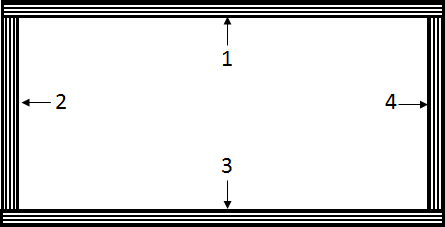
\includegraphics{boxBeamGeom.png}\hfill}
\begin{quote}\begin{description}
\item[{Args}] \leavevmode
\end{description}\end{quote}
\begin{itemize}
\item {} 
\emph{xsect (obj)}: The cross-section object to be meshed.

\item {} 
\emph{meshSize (int)}: The maximum aspect ratio an element can have

\item {} \begin{description}
\item[{\emph{x0 (float)}: The non-dimensional starting point of the cross-section}] \leavevmode
on the airfoil.

\end{description}

\item {} \begin{description}
\item[{\emph{xf (float)}: The non-dimesnional ending point of the cross-section}] \leavevmode
on the airfoil.

\end{description}

\item {} \begin{description}
\item[{\emph{matlib (obj)}: The material library object used to create CQUADX}] \leavevmode
elements.

\end{description}

\end{itemize}
\begin{quote}\begin{description}
\item[{Returns}] \leavevmode
\end{description}\end{quote}
\begin{itemize}
\item {} 
None

\end{itemize}

\end{fulllineitems}

\index{laminate() (AeroComBAT.Structures.Mesher method)}

\begin{fulllineitems}
\phantomsection\label{structures:AeroComBAT.Structures.Mesher.laminate}\pysiglinewithargsret{\bfcode{laminate}}{\emph{xsect}, \emph{meshSize}, \emph{x0}, \emph{xf}, \emph{matlib}}{}
Meshes laminate cross-section.

This method meshes a simple laminate cross-section. It is assumed that
the unit normal vector of the laminate points in the y-direction. This
method only requires one laminate, which can take any shape. The cross-
section geometry can be seen below:

{\hfill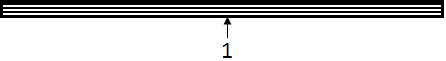
\includegraphics{laminateGeom.png}\hfill}
\begin{quote}\begin{description}
\item[{Args}] \leavevmode
\end{description}\end{quote}
\begin{itemize}
\item {} 
\emph{xsect (obj)}: The cross-section object to be meshed.

\item {} 
\emph{meshSize (int)}: The maximum aspect ratio an element can have

\item {} \begin{description}
\item[{\emph{x0 (float)}: The non-dimensional starting point of the cross-section}] \leavevmode
on the airfoil.

\end{description}

\item {} \begin{description}
\item[{\emph{xf (float)}: The non-dimesnional ending point of the cross-section}] \leavevmode
on the airfoil.

\end{description}

\item {} \begin{description}
\item[{\emph{matlib (obj)}: The material library object used to create CQUADX}] \leavevmode
elements.

\end{description}

\end{itemize}
\begin{quote}\begin{description}
\item[{Returns}] \leavevmode
\end{description}\end{quote}
\begin{itemize}
\item {} 
None

\end{itemize}

\end{fulllineitems}

\index{rectBoxBeam() (AeroComBAT.Structures.Mesher method)}

\begin{fulllineitems}
\phantomsection\label{structures:AeroComBAT.Structures.Mesher.rectBoxBeam}\pysiglinewithargsret{\bfcode{rectBoxBeam}}{\emph{xsect}, \emph{meshSize}, \emph{x0}, \emph{xf}, \emph{matlib}}{}
Meshes a box beam cross-section.

This method meshes a similar cross-section as the boxBeam method. The
geometry of this cross-section can be seen below. The interfaces
between the laminates is different, and more restrictive. In this case
all of the laminates must have the same number of plies, which must
also all be the same thickness.

{\hfill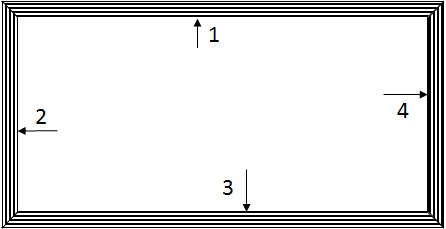
\includegraphics{rectBoxGeom.png}\hfill}
\begin{quote}\begin{description}
\item[{Args}] \leavevmode
\end{description}\end{quote}
\begin{itemize}
\item {} 
\emph{xsect (obj)}: The cross-section object to be meshed.

\item {} 
\emph{meshSize (int)}: The maximum aspect ratio an element can have

\item {} \begin{description}
\item[{\emph{x0 (float)}: The non-dimensional starting point of the cross-section}] \leavevmode
on the airfoil.

\end{description}

\item {} \begin{description}
\item[{\emph{xf (float)}: The non-dimesnional ending point of the cross-section}] \leavevmode
on the airfoil.

\end{description}

\item {} \begin{description}
\item[{\emph{matlib (obj)}: The material library object used to create CQUADX}] \leavevmode
elements.

\end{description}

\end{itemize}
\begin{quote}\begin{description}
\item[{Returns}] \leavevmode
\end{description}\end{quote}
\begin{itemize}
\item {} 
None

\end{itemize}

\end{fulllineitems}


\end{fulllineitems}



\subsection{CROSS-SECTION}
\label{structures:cross-section}\index{XSect (class in AeroComBAT.Structures)}

\begin{fulllineitems}
\phantomsection\label{structures:AeroComBAT.Structures.XSect}\pysiglinewithargsret{\strong{class }\code{AeroComBAT.Structures.}\bfcode{XSect}}{\emph{XID}, \emph{Airfoil}, \emph{xdim}, \emph{laminates}, \emph{matlib}, \emph{**kwargs}}{}
Creates a beam cross-section object,

This cross-section can be made of multiple materials which can be in
general anisotropic. This is the main workhorse within the structures
library.
\begin{quote}\begin{description}
\item[{Attributes}] \leavevmode
\end{description}\end{quote}
\begin{itemize}
\item {} \begin{description}
\item[{\emph{Color (touple)}: A length 3 touple used to define the color of the}] \leavevmode
cross-section.

\end{description}

\item {} \begin{description}
\item[{\emph{Airfoil (obj)}: The airfoil object used to define the OML of the cross-}] \leavevmode
section.

\end{description}

\item {} \begin{description}
\item[{\emph{typeXSect (str)}: Defines what type of cross-section is to be used.}] \leavevmode
Currently the only supported type is `box'.

\end{description}

\item {} \begin{description}
\item[{\emph{normalVector (1x3 np.array{[}float{]})}: Expresses the normal vector of the}] \leavevmode
cross-section.

\end{description}

\item {} \begin{description}
\item[{\emph{nodeDict (dict)}: A dictionary of all nodes used to descretize the}] \leavevmode
cross-section surface. The keys are the NIDs and the values stored
are the Node objects.

\end{description}

\item {} \begin{description}
\item[{\emph{elemDict (dict)}: A dictionary of all elements used to descretize the}] \leavevmode
cross-section surface. the keys are the EIDs and the values stored
are the element objects.

\end{description}

\item {} \begin{description}
\item[{\emph{X (ndx6 np.array{[}float{]})}: A very large 2D array. This is one of the}] \leavevmode
results of the cross-sectional analysis. This array relays the
force and moment resultants applied to the cross-section to the
nodal warping displacements exhibited by the cross-section.

\end{description}

\item {} \begin{description}
\item[{\emph{Y (6x6 np.array{[}float{]})}: This array relays the force and moment}] \leavevmode
resultants applied to the cross-section to the rigid section
strains and curvatures exhibited by the cross-section.

\end{description}

\item {} \begin{description}
\item[{\emph{dXdz (ndx6 np.array{[}float{]})}: A very large 2D array. This is one of the}] \leavevmode
results of the cross-sectional analysis. This array relays the
force and moment resultants applied to the cross-section to the
gradient of the nodal warping displacements exhibited by the
cross-section with respect to the beam axis.

\end{description}

\item {} \begin{description}
\item[{\emph{xt (float)}: The x-coordinate of the tension center (point at which}] \leavevmode
tension and bending are decoupled)

\end{description}

\item {} \begin{description}
\item[{\emph{yt (float)}: The y-coordinate of the tension center (point at which}] \leavevmode
tension and bending are decoupled)

\end{description}

\item {} \begin{description}
\item[{\emph{xs (float)}: The x-coordinate of the shear center (point at which shear}] \leavevmode
and torsion are decoupled)

\end{description}

\item {} \begin{description}
\item[{\emph{ys (float)}: The y-coordinate of the shear center (point at which shear}] \leavevmode
and torsion are decoupled)

\end{description}

\item {} \begin{description}
\item[{\emph{refAxis (3x1 np.array{[}float{]})}: A column vector containing the reference}] \leavevmode
axis for the beam.

\end{description}

\item {} \begin{description}
\item[{\emph{bendAxes (2x3 np.array{[}float{]})}: Contains two row vectors about which}] \leavevmode
bending from one axis is decoupled from bending about the other.

\end{description}

\item {} \begin{description}
\item[{\emph{F\_raw (6x6 np.array{[}float{]})}: The 6x6 compliance matrix that results}] \leavevmode
from cross-sectional analysis. This is the case where the reference
axis is at the origin.

\end{description}

\item {} \begin{description}
\item[{\emph{K\_raw (6x6 np.array{[}float{]})}: The 6x6 stiffness matrix that results}] \leavevmode
from cross-sectional analysis. This is the case where the reference
axis is at the origin.

\end{description}

\item {} \begin{description}
\item[{\emph{F (6x6 np.array{[}float{]})}: The 6x6 compliance matrix for the cross-}] \leavevmode
section about the reference axis. The reference axis is by default
at the shear center.

\end{description}

\item {} \begin{description}
\item[{\emph{K (6x6 np.array{[}float{]})}: The 6x6 stiffness matrix for the cross-}] \leavevmode
section about the reference axis. The reference axis is by default
at the shear center.

\end{description}

\item {} \begin{description}
\item[{\emph{T1 (3x6 np.array{[}float{]})}: The transformation matrix that converts}] \leavevmode
strains and curvatures from the local xsect origin to the reference
axis.

\end{description}

\item {} \begin{description}
\item[{\emph{T2 (3x6 np.array{[}float{]})}: The transformation matrix that converts}] \leavevmode
forces and moments from the local xsect origin to the reference
axis.

\end{description}

\item {} \begin{description}
\item[{\emph{x\_m (1x3 np.array{[}float{]})}: Center of mass of the cross-section about in}] \leavevmode
the local xsect CSYS

\end{description}

\item {} \begin{description}
\item[{\emph{M (6x6 np.array{[}float{]})}: This mass matrix relays linear and angular}] \leavevmode
velocities to linear and angular momentum of the cross-section.

\end{description}

\end{itemize}
\begin{quote}\begin{description}
\item[{Methods}] \leavevmode
\end{description}\end{quote}
\begin{itemize}
\item {} \begin{description}
\item[{\emph{resetResults}: This method resets all results (displacements, strains}] \leavevmode
and stresse) within the elements used by the cross-section object.

\end{description}

\item {} \begin{description}
\item[{\emph{calcWarpEffects}: Given applied force and moment resultants, this method}] \leavevmode
calculates the warping displacement, 3D strains and 3D stresses
within the elements used by the cross-section.

\end{description}

\item {} \begin{description}
\item[{\emph{printSummary}: This method is used to print characteristic attributes of}] \leavevmode
the object. This includes the elastic, shear and mass centers, as
well as the stiffness matrix and mass matrix.

\end{description}

\item {} \begin{description}
\item[{\emph{plotRigid}: This method plots the rigid cross-section shape, typically}] \leavevmode
in conjunction with a full beam model.

\end{description}

\item {} \begin{description}
\item[{\emph{plotWarped}: This method plots the warped cross-section including a}] \leavevmode
contour criteria, typically in conjuction with the results of the
displacement of a full beam model.

\end{description}

\end{itemize}
\index{\_\_init\_\_() (AeroComBAT.Structures.XSect method)}

\begin{fulllineitems}
\phantomsection\label{structures:AeroComBAT.Structures.XSect.__init__}\pysiglinewithargsret{\bfcode{\_\_init\_\_}}{\emph{XID}, \emph{Airfoil}, \emph{xdim}, \emph{laminates}, \emph{matlib}, \emph{**kwargs}}{}
Instantiates a cross-section object.

The constructor for the class is effectively responsible for creating
the 2D desretized mesh of the cross-section. It is important to note
that while meshing technically occurs in the constructor, the work is
handeled by another class altogether. While not
computationally heavily intensive in itself, it is responsible for
creating all of the framework for the cross-sectional analysis.
\begin{quote}\begin{description}
\item[{Args}] \leavevmode
\end{description}\end{quote}
\begin{itemize}
\item {} 
\emph{XID (int)}: The cross-section integer identifier.

\item {} \begin{description}
\item[{\emph{Airfoil (obj)}: An airfoil object used to determine the OML shape of}] \leavevmode
the cross-section.

\end{description}

\item {} \begin{description}
\item[{\emph{xdim (1x2 array{[}float{]})}: The non-dimensional starting and stoping}] \leavevmode
points of the cross-section. In other words, if you wanted to
have your cross-section start at the 1/4 chord and run to the
3/4 chord of your airfoil, xdim would look like xdim={[}0.25,0.75{]}

\end{description}

\item {} \begin{description}
\item[{\emph{laminates (1xN array{[}obj{]})}: Laminate objects used to create the}] \leavevmode
descretized mesh surface. Do not repeat a laminate within this
array! It will referrence this object multiple times and not
mesh the cross-section properly then!

\end{description}

\item {} 
\emph{matlib (obj)}: A material library

\item {} \begin{description}
\item[{\emph{typeXSect (str)}: The general shape the cross-section should take.}] \leavevmode
Note that currently only a box beam profile is supported.
More shapes and the ability to add stiffeners to the
cross-section will come in later updates.

\end{description}

\item {} \begin{description}
\item[{\emph{meshSize (int)}: The maximum aspect ratio you would like your 2D}] \leavevmode
CQUADX elements to exhibit within the cross-section.

\end{description}

\end{itemize}
\begin{quote}\begin{description}
\item[{Returns}] \leavevmode
\end{description}\end{quote}
\begin{itemize}
\item {} 
None

\end{itemize}

\end{fulllineitems}

\index{calcWarpEffects() (AeroComBAT.Structures.XSect method)}

\begin{fulllineitems}
\phantomsection\label{structures:AeroComBAT.Structures.XSect.calcWarpEffects}\pysiglinewithargsret{\bfcode{calcWarpEffects}}{\emph{**kwargs}}{}
Calculates displacements, stresses, and strains for applied forces

The second most powerful method of the XSect class. After an analysis
is run, the FEM class stores force and moment resultants within the
beam element objects. From there, warping displacement, strain and
stress can be determined within the cross-section at any given location
within the beam using this method. This method will take a while though
as it has to calculate 4 displacements and 24 stresses and strains for
every element within the cross-section. Keep that in mind when you are
surveying your beam or wing for displacements, stresses and strains.
\begin{quote}\begin{description}
\item[{Args}] \leavevmode
\end{description}\end{quote}
\begin{itemize}
\item {} \begin{description}
\item[{\emph{force (6x1 np.array{[}float{]})}: This is the internal force and moment}] \leavevmode
resultant experienced by the cross-section.

\end{description}

\end{itemize}
\begin{quote}\begin{description}
\item[{Returns}] \leavevmode
\end{description}\end{quote}
\begin{itemize}
\item {} 
None

\end{itemize}

\end{fulllineitems}

\index{plotRigid() (AeroComBAT.Structures.XSect method)}

\begin{fulllineitems}
\phantomsection\label{structures:AeroComBAT.Structures.XSect.plotRigid}\pysiglinewithargsret{\bfcode{plotRigid}}{\emph{**kwargs}}{}
Plots the rigid cross-section along a beam.

This method is very useful for visually debugging a structural model.
It will plot out the rigid cross-section in 3D space with regards to
the reference axis.
\begin{quote}\begin{description}
\item[{Args}] \leavevmode
\end{description}\end{quote}
\begin{itemize}
\item {} \begin{description}
\item[{\emph{x (1x3 np.array{[}float{]})}: The rigid location on your beam you are}] \leavevmode
trying to plot:

\end{description}

\item {} \begin{description}
\item[{\emph{beam\_axis (1x3 np.array{[}float{]})}: The vector pointing in the}] \leavevmode
direction of your beam axis.

\end{description}

\item {} 
\emph{figName (str)}: The name of the figure.

\item {} \begin{description}
\item[{\emph{wireMesh (bool)}: A boolean to determine of the wiremesh outline}] \leavevmode
should be plotted.*

\end{description}

\end{itemize}
\begin{quote}\begin{description}
\item[{Returns}] \leavevmode
\end{description}\end{quote}
\begin{itemize}
\item {} 
\emph{(fig)}: Plots the cross-section in a mayavi figure.

\end{itemize}

\begin{notice}{note}{Note:}
Because of how the mayavi wireframe keyword works, it will
\end{notice}

apear as though the cross-section is made of triangles as opposed to
quadrilateras. Fear not! They are made of quads, the wireframe is just
plotted as triangles.

\end{fulllineitems}

\index{plotWarped() (AeroComBAT.Structures.XSect method)}

\begin{fulllineitems}
\phantomsection\label{structures:AeroComBAT.Structures.XSect.plotWarped}\pysiglinewithargsret{\bfcode{plotWarped}}{\emph{**kwargs}}{}
Plots the warped cross-section along a beam.

Once an analysis has been completed, this method can be utilized in
order to plot the results anywhere along the beam.
\begin{quote}\begin{description}
\item[{Args}] \leavevmode
\end{description}\end{quote}
\begin{itemize}
\item {} \begin{description}
\item[{\emph{displScale (float)}: The scale by which all rotations and}] \leavevmode
displacements will be mutliplied in order make it visually
easier to detect displacements.

\end{description}

\item {} \begin{description}
\item[{\emph{x (1x3 np.array{[}float{]})}: The rigid location on your beam you are}] \leavevmode
trying to plot:

\end{description}

\item {} \begin{description}
\item[{\emph{U (1x6 np.array{[}float{]})}: The rigid body displacements and rotations}] \leavevmode
experienced by the cross-section.

\end{description}

\item {} \begin{description}
\item[{\emph{beam\_axis (1x3 np.array{[}float{]})}: The vector pointing in the}] \leavevmode
direction of your beam axis.

\end{description}

\item {} \begin{description}
\item[{\emph{contour (str)}: Determines what value is to be plotted during as a}] \leavevmode
contour in the cross-section.

\end{description}

\item {} 
\emph{figName (str)}: The name of the figure.

\item {} \begin{description}
\item[{\emph{wireMesh (bool)}: A boolean to determine of the wiremesh outline}] \leavevmode
should be plotted.*

\end{description}

\item {} \begin{description}
\item[{\emph{contLim (1x2 array{[}float{]})}: Describes the upper and lower bounds of}] \leavevmode
contour color scale.

\end{description}

\item {} \begin{description}
\item[{\emph{warpScale (float)}: The scaling factor by which all warping}] \leavevmode
displacements in the cross-section will be multiplied.

\end{description}

\end{itemize}
\begin{quote}\begin{description}
\item[{Returns}] \leavevmode
\end{description}\end{quote}
\begin{itemize}
\item {} 
\emph{(fig)}: Plots the cross-section in a mayavi figure.

\end{itemize}

\begin{notice}{note}{Note:}
Because of how the mayavi wireframe keyword works, it will
\end{notice}

apear as though the cross-section is made of triangles as opposed to
quadrilateras. Fear not! They are made of quads, the wireframe is just
plotted as triangles.

\end{fulllineitems}

\index{printSummary() (AeroComBAT.Structures.XSect method)}

\begin{fulllineitems}
\phantomsection\label{structures:AeroComBAT.Structures.XSect.printSummary}\pysiglinewithargsret{\bfcode{printSummary}}{\emph{refAxis=True}, \emph{decimals=8}, \emph{**kwargs}}{}
Print characterisic information about the cross-section.

This method prints out characteristic information about the cross-
section objects. By default, the method will print out the location of
the reference axis, the shear, tension, and mass center. This method
if requested will also print the stiffness and mass matricies.
\begin{quote}\begin{description}
\item[{Args}] \leavevmode
\end{description}\end{quote}
\begin{itemize}
\item {} \begin{description}
\item[{\emph{refAxis (bool)}: Boolean to determine if the stiffness matrix}] \leavevmode
printed should be about the reference axis (True) or about the
local xsect origin (False).

\end{description}

\item {} \begin{description}
\item[{\emph{stiffMat (bool)}: Boolean to determine if the stiffness matrix}] \leavevmode
should be printed.

\end{description}

\item {} \begin{description}
\item[{\emph{tensCntr (bool)}: Boolean to determine if the location of the tension}] \leavevmode
center should be printed.

\end{description}

\item {} \begin{description}
\item[{\emph{shearCntr (bool)}: Boolean to determine if the location of the shear}] \leavevmode
center should be printed.

\end{description}

\item {} \begin{description}
\item[{\emph{massCntr (bool)}: Boolean to determine if the location of the mass}] \leavevmode
center should be printed.

\end{description}

\item {} \begin{description}
\item[{\emph{refAxisLoc (bool)}: Boolean to determine if the location of the}] \leavevmode
reference axis should be printed.

\end{description}

\end{itemize}
\begin{quote}\begin{description}
\item[{Returns}] \leavevmode
\end{description}\end{quote}
\begin{itemize}
\item {} 
\emph{(str)}: Prints out a string of information about the cross-section.

\end{itemize}

\end{fulllineitems}

\index{resetResults() (AeroComBAT.Structures.XSect method)}

\begin{fulllineitems}
\phantomsection\label{structures:AeroComBAT.Structures.XSect.resetResults}\pysiglinewithargsret{\bfcode{resetResults}}{}{}
Resets displacements, stress and strains within an xsect

This method clears all results (both warping, stress, and strain)
within the elements in the xsect object.
\begin{quote}\begin{description}
\item[{Args}] \leavevmode
\end{description}\end{quote}
\begin{itemize}
\item {} 
None

\end{itemize}
\begin{quote}\begin{description}
\item[{Returns}] \leavevmode
\end{description}\end{quote}
\begin{itemize}
\item {} 
None

\end{itemize}

\end{fulllineitems}

\index{xSectionAnalysis() (AeroComBAT.Structures.XSect method)}

\begin{fulllineitems}
\phantomsection\label{structures:AeroComBAT.Structures.XSect.xSectionAnalysis}\pysiglinewithargsret{\bfcode{xSectionAnalysis}}{\emph{**kwargs}}{}
Analyzes an initialized corss-section.

This is the main workhorse of the class. This method assembles the
finite element model generated using the meshing class, and solve the
HIGH dimensional equilibrium equations associated with the cross-
section. In doing so, it generates the warping displacement, the
section strain, and the gradient of the warping displacement along the
beam axis as a function of force-moment resultants. With these three
things, the 3D strains-\textgreater{}stresses can be recovered.

This method has been EXTENSIVELY tested and validated against
various sources (see theory guide for more info). Since this method
is so robust, the biggest limitation of the XSect class is what the
mesher is capable of meshing. Finally, keep in mind that due to the
high dimensionality of this problem, this method uses up a lot of
resources (primarily memory). If this method is taking too many
resources, choose a larger aspect ratio for your XSect initialization.
\begin{quote}\begin{description}
\item[{Args}] \leavevmode
\end{description}\end{quote}
\begin{itemize}
\item {} \begin{description}
\item[{\emph{ref\_ax (str or 1x2 array{[}float{]})}: Currently there are two supported}] \leavevmode
input types for this class. The first is the are string key-words.
These are `shearCntr', `massCntr', and `origin'. Currently
`shearCntr' is the default value. Also suported is the ability to
pass a length 2 array containing the x and y coordinates of the
reference axis relative to the origin. This would take the form of:
ref\_ax={[}1.,3.{]} to put the reference axis at x,y = 1.,3.

\end{description}

\end{itemize}
\begin{quote}\begin{description}
\item[{Returns}] \leavevmode
\end{description}\end{quote}
\begin{itemize}
\item {} 
None

\end{itemize}

\end{fulllineitems}


\end{fulllineitems}



\subsection{TIMOSHENKO BEAM}
\label{structures:timoshenko-beam}\index{TBeam (class in AeroComBAT.Structures)}

\begin{fulllineitems}
\phantomsection\label{structures:AeroComBAT.Structures.TBeam}\pysiglinewithargsret{\strong{class }\code{AeroComBAT.Structures.}\bfcode{TBeam}}{\emph{EID}, \emph{x1}, \emph{x2}, \emph{xsect}, \emph{SBID=0}, \emph{nid1=0}, \emph{nid2=1}, \emph{chordVec=array({[} 1.}, \emph{0.}, \emph{0.{]})}}{}
Creates a Timoshenko beam finite element object.

The primary beam finite element used by AeroComBAT, this beam element is
similar to the Euler-Bernoulli beam finite element most are farmiliar with,
with the exception that it has the ability to experience shear deformation
in addition to just bending.
\begin{quote}\begin{description}
\item[{Attributes}] \leavevmode
\end{description}\end{quote}
\begin{itemize}
\item {} 
\emph{type (str)}:String describing the type of beam element being used.

\item {} \begin{description}
\item[{\emph{U1 (dict)}: This dictionary contains the results of an analysis set. The}] \leavevmode
keys are the string names of the analysis and the values stored are
6x1 np.array{[}float{]} vectors containing the 3 displacements and
3 rotations at the first node.

\end{description}

\item {} \begin{description}
\item[{\emph{U2 (dict)}: This dictionary contains the results of an analysis set. The}] \leavevmode
keys are the string names of the analysis and the values stored are
6x1 np.array{[}float{]} vectors containing the 3 displacements and
3 rotations at the second node.

\end{description}

\item {} \begin{description}
\item[{\emph{Umode1 (dict)}: This dictionary contains the results of a modal analysis}] \leavevmode
set. The keys are the string names of the analysis and the values
stored are 6xN np.array{[}float{]}. The columns of the array are the
displacements and rotations at the first node associated with the
particular mode.

\end{description}

\item {} \begin{description}
\item[{\emph{Umode2 (dict)}: This dictionary contains the results of a modal analysis}] \leavevmode
set. The keys are the string names of the analysis and the values
stored are 6xN np.array{[}float{]}. The columns of the array are the
displacements and rotations at the second node associated with the
particular mode.

\end{description}

\item {} \begin{description}
\item[{\emph{F1 (dict)}: This dictionary contains the results of an analysis set. The}] \leavevmode
keys are the string names of the analysis and the values stored are
6x1 np.array{[}float{]} vectors containing the 3 internal forces and
3 moments at the first node.

\end{description}

\item {} \begin{description}
\item[{\emph{F2 (dict)}: This dictionary contains the results of an analysis set. The}] \leavevmode
keys are the string names of the analysis and the values stored are
6x1 np.array{[}float{]} vectors containing the 3 internal forces and
3 moments at the second node.

\end{description}

\item {} \begin{description}
\item[{\emph{Fmode1 (dict)}: This dictionary contains the results of a modal analysis}] \leavevmode
set. The keys are the string names of the analysis and the values
stored are 6xN np.array{[}float{]}. The columns of the array are the
forces and moments at the first node associated with the
particular mode.*

\end{description}

\item {} \begin{description}
\item[{\emph{Fmode2 (dict)}: This dictionary contains the results of a modal analysis}] \leavevmode
set. The keys are the string names of the analysis and the values
stored are 6xN np.array{[}float{]}. The columns of the array are the
forces and moments at the second node associated with the
particular mode.*

\end{description}

\item {} \begin{description}
\item[{\emph{xsect (obj)}: The cross-section object used to determine the beams}] \leavevmode
stiffnesses.

\end{description}

\item {} 
\emph{EID (int)}: The element ID of the beam.

\item {} 
\emph{SBID (int)}: The associated Superbeam ID the beam object belongs to.

\item {} 
\emph{n1 (obj)}: The first nodal object used by the beam.

\item {} 
\emph{n2 (obj)}: The second nodal object used by the beam.

\item {} 
\emph{Fe (12x1 np.array{[}float{]})}: The distributed force vector of the element

\item {} 
\emph{Ke (12x12 np.array{[}float{]})}: The stiffness matrix of the beam.

\item {} \begin{description}
\item[{\emph{Keg (12x12 np.array{[}float{]})}: The geometric stiffness matrix of the}] \leavevmode
beam. Used for beam buckling calculations.

\end{description}

\item {} 
\emph{Me (12x12 np.array{[}float{]})}: The mass matrix of the beam.

\item {} 
\emph{h (float)}: The magnitude length of the beam element.

\item {} \begin{description}
\item[{\emph{xbar (float)}: The unit vector pointing in the direction of the rigid}] \leavevmode
beam.

\end{description}

\item {} 
\emph{T (12x12 np.array{[}float{]})}:

\end{itemize}
\begin{quote}\begin{description}
\item[{Methods}] \leavevmode
\end{description}\end{quote}
\begin{itemize}
\item {} \begin{description}
\item[{\emph{printSummary}: This method prints out characteristic attributes of the}] \leavevmode
beam finite element.

\end{description}

\item {} 
\emph{plotRigidBeam}: Plots the the shape of the rigid beam element.

\item {} 
\emph{plotDisplBeam}: Plots the deformed shape of the beam element.

\item {} \begin{description}
\item[{\emph{printInternalForce}: Prints the internal forces of the beam element for}] \leavevmode
a given analysis set

\end{description}

\end{itemize}

\begin{notice}{note}{Note:}
The force and moments in the Fmode1 and Fmode2 could be completely
\end{notice}

fictitious and be left as an artifact to fascilitate plotting of warped
cross-sections. DO NOT rely on this information being meaningful.
\index{\_\_init\_\_() (AeroComBAT.Structures.TBeam method)}

\begin{fulllineitems}
\phantomsection\label{structures:AeroComBAT.Structures.TBeam.__init__}\pysiglinewithargsret{\bfcode{\_\_init\_\_}}{\emph{EID}, \emph{x1}, \emph{x2}, \emph{xsect}, \emph{SBID=0}, \emph{nid1=0}, \emph{nid2=1}, \emph{chordVec=array({[} 1.}, \emph{0.}, \emph{0.{]})}}{}
Instantiates a timoshenko beam element.

This method instatiates a finite element timoshenko beam element.
Currently the beam must be oriented along the global y-axis, however
full 3D orientation support for frames is in progress.
\begin{quote}\begin{description}
\item[{Args}] \leavevmode
\end{description}\end{quote}
\begin{itemize}
\item {} \begin{description}
\item[{\emph{x1 (1x3 np.array{[}float{]})}: The 3D coordinates of the first beam}] \leavevmode
element node.

\end{description}

\item {} \begin{description}
\item[{\emph{x2 (1x3 np.array{[}float{]})}: The 3D coordinates of the second beam}] \leavevmode
element node.

\end{description}

\item {} \begin{description}
\item[{\emph{xsect (obj)}: The cross-section object used to determine stiffnes}] \leavevmode
and mass properties for the beam.

\end{description}

\item {} 
\emph{EID (int)}: The integer identifier for the beam.

\item {} 
\emph{SBID (int)}: The associated superbeam ID.

\item {} 
\emph{nid1 (int)}: The first node ID

\item {} 
\emph{nid2 (int)}: The second node ID

\end{itemize}
\begin{quote}\begin{description}
\item[{Returns}] \leavevmode
\end{description}\end{quote}
\begin{itemize}
\item {} 
None

\end{itemize}

\end{fulllineitems}

\index{plotDisplBeam() (AeroComBAT.Structures.TBeam method)}

\begin{fulllineitems}
\phantomsection\label{structures:AeroComBAT.Structures.TBeam.plotDisplBeam}\pysiglinewithargsret{\bfcode{plotDisplBeam}}{\emph{**kwargs}}{}
Plots the displaced beam in 3D space.

This method plots the deformed beam finite element in 3D space. It is
not typically called by the beam object but by a SuperBeam object
or even a WingSection object.
\begin{quote}\begin{description}
\item[{Args}] \leavevmode
\end{description}\end{quote}
\begin{itemize}
\item {} \begin{description}
\item[{\emph{environment (str)}: Determines what environment is to be used to}] \leavevmode
plot the beam in 3D space. Currently only mayavi is supported.

\end{description}

\item {} 
\emph{figName (str)}: The name of the figure in which the beam will apear.

\item {} \begin{description}
\item[{\emph{clr (1x3 touple(float))}: This touple contains three floats running}] \leavevmode
from 0 to 1 in order to generate a color mayavi can plot.

\end{description}

\item {} \begin{description}
\item[{\emph{displScale (float)}: The scaling factor for the deformation}] \leavevmode
experienced by the beam.

\end{description}

\item {} \begin{description}
\item[{\emph{mode (int)}: Determines what mode to plot. By default the mode is 0}] \leavevmode
implying a non-eigenvalue solution should be plotted.

\end{description}

\end{itemize}
\begin{quote}\begin{description}
\item[{Returns}] \leavevmode
\end{description}\end{quote}
\begin{itemize}
\item {} 
\emph{(fig)}: The mayavi figure of the beam.

\end{itemize}

\end{fulllineitems}

\index{plotRigidBeam() (AeroComBAT.Structures.TBeam method)}

\begin{fulllineitems}
\phantomsection\label{structures:AeroComBAT.Structures.TBeam.plotRigidBeam}\pysiglinewithargsret{\bfcode{plotRigidBeam}}{\emph{**kwargs}}{}
Plots the rigid beam in 3D space.

This method plots the beam finite element in 3D space. It is not
typically called by the beam object but by a SuperBeam object or
even a WingSection object.
\begin{quote}\begin{description}
\item[{Args}] \leavevmode
\end{description}\end{quote}
\begin{itemize}
\item {} \begin{description}
\item[{\emph{environment (str)}: Determines what environment is to be used to}] \leavevmode
plot the beam in 3D space. Currently only mayavi is supported.

\end{description}

\item {} 
\emph{figName (str)}: The name of the figure in which the beam will apear.

\item {} \begin{description}
\item[{\emph{clr (1x3 touple(float))}: This touple contains three floats running}] \leavevmode
from 0 to 1 in order to generate a color mayavi can plot.

\end{description}

\end{itemize}
\begin{quote}\begin{description}
\item[{Returns}] \leavevmode
\end{description}\end{quote}
\begin{itemize}
\item {} 
\emph{(fig)}: The mayavi figure of the beam.

\end{itemize}

\end{fulllineitems}

\index{printInternalForce() (AeroComBAT.Structures.TBeam method)}

\begin{fulllineitems}
\phantomsection\label{structures:AeroComBAT.Structures.TBeam.printInternalForce}\pysiglinewithargsret{\bfcode{printInternalForce}}{\emph{**kwargs}}{}
Prints the internal forces and moments in the beam.

For a particular analysis set, this method prints out the force and
moment resultants at both nodes of the beam.
\begin{quote}\begin{description}
\item[{Args}] \leavevmode
\end{description}\end{quote}
\begin{itemize}
\item {} \begin{description}
\item[{\emph{analysis\_name (str)}: The analysis name for which the forces are}] \leavevmode
being surveyed.

\end{description}

\end{itemize}
\begin{quote}\begin{description}
\item[{Returns}] \leavevmode
\end{description}\end{quote}
\begin{itemize}
\item {} \begin{description}
\item[{\emph{(str)}: This is a print out of the internal forces and moments}] \leavevmode
within the beam element.

\end{description}

\end{itemize}

\end{fulllineitems}

\index{printSummary() (AeroComBAT.Structures.TBeam method)}

\begin{fulllineitems}
\phantomsection\label{structures:AeroComBAT.Structures.TBeam.printSummary}\pysiglinewithargsret{\bfcode{printSummary}}{\emph{decimals=8}, \emph{**kwargs}}{}
Prints out characteristic information about the beam element.

This method by default prints out the EID, XID, SBID and the NIDs along
with the nodes associated coordinates. Upon request, it can also print
out the beam element stiffness, geometric stiffness, mass matricies and
distributed force vector.
\begin{quote}\begin{description}
\item[{Args}] \leavevmode
\end{description}\end{quote}
\begin{itemize}
\item {} \begin{description}
\item[{\emph{nodeCoord (bool)}: A boolean to determine if the node coordinate}] \leavevmode
information should also be printed.

\end{description}

\item {} \begin{description}
\item[{\emph{Ke (bool)}: A boolean to determine if the element stiffness matrix}] \leavevmode
should be printed.

\end{description}

\item {} \begin{description}
\item[{\emph{Keg (bool)}: A boolean to determine if the element gemoetric}] \leavevmode
stiffness matrix should be printed.

\end{description}

\item {} \begin{description}
\item[{\emph{Me (bool)}: A boolean to determine if the element mass matrix}] \leavevmode
should be printed.

\end{description}

\item {} \begin{description}
\item[{\emph{Fe (bool)}: A boolean to determine if the element distributed force}] \leavevmode
and moment vector should be printed.

\end{description}

\end{itemize}
\begin{quote}\begin{description}
\item[{Returns}] \leavevmode
\end{description}\end{quote}
\begin{itemize}
\item {} 
\emph{(str)}: Printed summary of the requested attributes.

\end{itemize}

\end{fulllineitems}


\end{fulllineitems}



\subsection{SUPER-BEAM}
\label{structures:super-beam}\index{SuperBeam (class in AeroComBAT.Structures)}

\begin{fulllineitems}
\phantomsection\label{structures:AeroComBAT.Structures.SuperBeam}\pysiglinewithargsret{\strong{class }\code{AeroComBAT.Structures.}\bfcode{SuperBeam}}{\emph{SBID}, \emph{x1}, \emph{x2}, \emph{xsect}, \emph{noe}, \emph{btype='Tbeam'}, \emph{sNID=1}, \emph{sEID=1}, \emph{**kwargs}}{}
Create a superbeam object.

The superbeam object is mainly to fascilitate creating a whole series of
beam objects along  the same line.
\begin{quote}\begin{description}
\item[{Attributes}] \leavevmode
\end{description}\end{quote}
\begin{itemize}
\item {} 
\emph{type (str)}: The object type, a `SuperBeam'.

\item {} 
\emph{btype (str)}: The beam element type of the elements in the superbeam.

\item {} 
\emph{SBID (int)}: The integer identifier for the superbeam.

\item {} 
\emph{sNID (int)}: The starting NID of the superbeam.

\item {} 
\emph{enid (int)}: The ending NID of the superbeam.

\item {} \begin{description}
\item[{\emph{xsect (obj)}: The cross-section object referenced by the beam elements}] \leavevmode
in the superbeam.

\end{description}

\item {} 
\emph{noe (int)}: Number of elements in the beam.

\item {} 
\emph{NIDs2EIDs (dict)}: Mapping of NIDs to beam EIDs within the superbeam

\item {} \begin{description}
\item[{\emph{x1 (1x3 np.array{[}float{]})}: The 3D coordinate of the first point on the}] \leavevmode
superbeam.

\end{description}

\item {} \begin{description}
\item[{\emph{x2 (1x3 np.array{[}float{]})}: The 3D coordinate of the last point on the}] \leavevmode
superbeam.

\end{description}

\item {} \begin{description}
\item[{\emph{sEID (int)}: The integer identifier for the first beam element in the}] \leavevmode
superbeam.

\end{description}

\item {} \begin{description}
\item[{\emph{elems (dict)}: A dictionary of all beam elements within the superbeam.}] \leavevmode
The keys are the EIDs and the values are the corresponding beam
elements.

\end{description}

\item {} \begin{description}
\item[{\emph{xbar (1x3 np.array{[}float{]})}: The vector pointing along the axis of the}] \leavevmode
superbeam.

\end{description}

\end{itemize}
\begin{quote}\begin{description}
\item[{Methods}] \leavevmode
\end{description}\end{quote}
\begin{itemize}
\item {} 
\emph{getBeamCoord}: Returns the 3D coordinate of a point along the superbeam.

\item {} \begin{description}
\item[{\emph{printInternalForce}: Prints all internal forces and moments at every}] \leavevmode
node in the superbeam.

\end{description}

\item {} \begin{description}
\item[{\emph{writeDisplacements}: Writes all displacements and rotations in the}] \leavevmode
superbeam to a .csv

\end{description}

\item {} \begin{description}
\item[{\emph{getEIDatx}: Provided a non-dimensional point along the superbeam, this}] \leavevmode
method returns the local element EID and the non-dimensional
coordinate within that element.

\end{description}

\item {} \begin{description}
\item[{\emph{printSummary}: Prints all of the elements and node IDs within the beam}] \leavevmode
as well as the coordinates of those nodes.

\end{description}

\end{itemize}
\index{\_\_init\_\_() (AeroComBAT.Structures.SuperBeam method)}

\begin{fulllineitems}
\phantomsection\label{structures:AeroComBAT.Structures.SuperBeam.__init__}\pysiglinewithargsret{\bfcode{\_\_init\_\_}}{\emph{SBID}, \emph{x1}, \emph{x2}, \emph{xsect}, \emph{noe}, \emph{btype='Tbeam'}, \emph{sNID=1}, \emph{sEID=1}, \emph{**kwargs}}{}
Creates a superelement object.

This method instantiates a superelement. What it effectively does is
mesh a line provided the starting and ending points along that line.
Keep in mind that for now, only beams running parallel to the z-axis
are supported.
\begin{quote}\begin{description}
\item[{Args}] \leavevmode
\end{description}\end{quote}
\begin{itemize}
\item {} 
\emph{x1 (1x3 np.array{[}float{]})}: The starting coordinate of the beam.

\item {} 
\emph{x2 (1x3 np.array{[}float{]})}: The ending coordinate of the beam.

\item {} 
\emph{xsect (obj)}: The cross-section used throught the superbeam.

\item {} 
\emph{noe (int)}: The number of elements along the beam.

\item {} 
\emph{SBID (int)}: The integer identifier for the superbeam.

\item {} \begin{description}
\item[{\emph{btype (str)}: The beam type to be meshed. Currently only Tbeam types}] \leavevmode
are supported.

\end{description}

\item {} 
\emph{sNID (int)}: The starting NID for the superbeam.

\item {} 
\emph{sEID (int)}: The starting EID for the superbeam.

\end{itemize}
\begin{quote}\begin{description}
\item[{Returns}] \leavevmode
\end{description}\end{quote}
\begin{itemize}
\item {} 
None

\end{itemize}

\end{fulllineitems}

\index{getBeamCoord() (AeroComBAT.Structures.SuperBeam method)}

\begin{fulllineitems}
\phantomsection\label{structures:AeroComBAT.Structures.SuperBeam.getBeamCoord}\pysiglinewithargsret{\bfcode{getBeamCoord}}{\emph{x\_nd}}{}
Determine the global coordinate along superbeam.

Provided the non-dimensional coordinate along the beam, this method
returns the global coordinate at that point.
\begin{quote}\begin{description}
\item[{Args}] \leavevmode
\end{description}\end{quote}
\begin{itemize}
\item {} \begin{description}
\item[{\emph{x\_nd (float)}: The non-dimensional coordinate along the beam. Note}] \leavevmode
that x\_nd must be between zero and one.

\end{description}

\end{itemize}
\begin{quote}\begin{description}
\item[{Returns}] \leavevmode
\end{description}\end{quote}
\begin{itemize}
\item {} 
\emph{(1x3 np.array{[}float{]})}: The global coordinate corresponding to x\_nd

\end{itemize}

\end{fulllineitems}

\index{getEIDatx() (AeroComBAT.Structures.SuperBeam method)}

\begin{fulllineitems}
\phantomsection\label{structures:AeroComBAT.Structures.SuperBeam.getEIDatx}\pysiglinewithargsret{\bfcode{getEIDatx}}{\emph{x}}{}
Returns the beam EID at a non-dimensional x-location in the superbeam.

Provided the non-dimensional coordinate along the beam, this method
returns the global beam element EID, as well as the local non-
dimensional coordinate within the specific beam element.
\begin{quote}\begin{description}
\item[{Args}] \leavevmode
\end{description}\end{quote}
\begin{itemize}
\item {} 
\emph{x (float)}: The non-dimensional coordinate within the super-beam

\end{itemize}
\begin{quote}\begin{description}
\item[{Returns}] \leavevmode
\end{description}\end{quote}
\begin{itemize}
\item {} \begin{description}
\item[{\emph{EID (int)}: The EID of the element containing the non-dimensional}] \leavevmode
coordinate provided.

\end{description}

\item {} \begin{description}
\item[{\emph{local\_x\_nd (float)}: The non-dimensional coordinate within the beam}] \leavevmode
element associated with the provided non-dimensional coordinate
within the beam.

\end{description}

\end{itemize}

\end{fulllineitems}

\index{printInternalForce() (AeroComBAT.Structures.SuperBeam method)}

\begin{fulllineitems}
\phantomsection\label{structures:AeroComBAT.Structures.SuperBeam.printInternalForce}\pysiglinewithargsret{\bfcode{printInternalForce}}{\emph{**kwargs}}{}
Prints the internal forces and moments in the superbeam.

For every node within the superbeam, this method will print out the
internal forces and moments at those nodes.
\begin{quote}\begin{description}
\item[{Args}] \leavevmode
\end{description}\end{quote}
\begin{itemize}
\item {} \begin{description}
\item[{\emph{analysis\_name (str)}: The name of the analysis for which the forces}] \leavevmode
and moments are being surveyed.

\end{description}

\end{itemize}
\begin{quote}\begin{description}
\item[{Returns}] \leavevmode
\end{description}\end{quote}
\begin{itemize}
\item {} 
\emph{(str)}: Printed output expressing all forces and moments.

\end{itemize}

\end{fulllineitems}

\index{printSummary() (AeroComBAT.Structures.SuperBeam method)}

\begin{fulllineitems}
\phantomsection\label{structures:AeroComBAT.Structures.SuperBeam.printSummary}\pysiglinewithargsret{\bfcode{printSummary}}{\emph{decimals=8}, \emph{**kwargs}}{}
Prints out characteristic information about the super beam.

This method by default prints out the EID, XID, SBID and the NIDs along
with the nodes associated coordinates. Upon request, it can also print
out the beam element stiffness, geometric stiffness, mass matricies and
distributed force vector.
\begin{quote}\begin{description}
\item[{Args}] \leavevmode
\end{description}\end{quote}
\begin{itemize}
\item {} \begin{description}
\item[{\emph{nodeCoord (bool)}: A boolean to determine if the node coordinate}] \leavevmode
information should also be printed.

\end{description}

\item {} \begin{description}
\item[{\emph{Ke (bool)}: A boolean to determine if the element stiffness matrix}] \leavevmode
should be printed.

\end{description}

\item {} \begin{description}
\item[{\emph{Keg (bool)}: A boolean to determine if the element gemoetric}] \leavevmode
stiffness matrix should be printed.

\end{description}

\item {} \begin{description}
\item[{\emph{Me (bool)}: A boolean to determine if the element mass matrix}] \leavevmode
should be printed.

\end{description}

\item {} \begin{description}
\item[{\emph{Fe (bool)}: A boolean to determine if the element distributed force}] \leavevmode
and moment vector should be printed.

\end{description}

\end{itemize}
\begin{quote}\begin{description}
\item[{Returns}] \leavevmode
\end{description}\end{quote}
\begin{itemize}
\item {} 
\emph{(str)}: Printed summary of the requested attributes.

\end{itemize}

\end{fulllineitems}

\index{writeDisplacements() (AeroComBAT.Structures.SuperBeam method)}

\begin{fulllineitems}
\phantomsection\label{structures:AeroComBAT.Structures.SuperBeam.writeDisplacements}\pysiglinewithargsret{\bfcode{writeDisplacements}}{\emph{**kwargs}}{}
Write internal displacements and rotations to file.

For every node within the superbeam, this method will tabulate all of
the displacements and rotations and then write them to a file.
\begin{quote}\begin{description}
\item[{Args}] \leavevmode
\end{description}\end{quote}
\begin{itemize}
\item {} 
\emph{fileName (str)}: The name of the file where the data will be written.

\item {} \begin{description}
\item[{\emph{analysis\_name (str)}: The name of the analysis for which the}] \leavevmode
displacements and rotations are being surveyed.

\end{description}

\end{itemize}
\begin{quote}\begin{description}
\item[{Returns}] \leavevmode
\end{description}\end{quote}
\begin{itemize}
\item {} \begin{description}
\item[{\emph{fileName (file)}: This method doesn't actually return a file, rather}] \leavevmode
it writes the data to a file named ``fileName'' and saves it to the
working directory.

\end{description}

\end{itemize}

\end{fulllineitems}

\index{writeForcesMoments() (AeroComBAT.Structures.SuperBeam method)}

\begin{fulllineitems}
\phantomsection\label{structures:AeroComBAT.Structures.SuperBeam.writeForcesMoments}\pysiglinewithargsret{\bfcode{writeForcesMoments}}{\emph{**kwargs}}{}
Write internal force and moments to file.

For every node within the superbeam, this method will tabulate all of
the forces and moments and then write them to a file.
\begin{quote}\begin{description}
\item[{Args}] \leavevmode
\end{description}\end{quote}
\begin{itemize}
\item {} 
\emph{fileName (str)}: The name of the file where the data will be written.

\item {} \begin{description}
\item[{\emph{analysis\_name (str)}: The name of the analysis for which the}] \leavevmode
forces and moments are being surveyed.

\end{description}

\end{itemize}
\begin{quote}\begin{description}
\item[{Returns}] \leavevmode
\end{description}\end{quote}
\begin{itemize}
\item {} \begin{description}
\item[{\emph{fileName (file)}: This method doesn't actually return a file, rather}] \leavevmode
it writes the data to a file named ``fileName'' and saves it to the
working directory.

\end{description}

\end{itemize}

\end{fulllineitems}


\end{fulllineitems}



\subsection{WING SECTION}
\label{structures:wing-section}\index{WingSection (class in AeroComBAT.Structures)}

\begin{fulllineitems}
\phantomsection\label{structures:AeroComBAT.Structures.WingSection}\pysiglinewithargsret{\strong{class }\code{AeroComBAT.Structures.}\bfcode{WingSection}}{\emph{x1}, \emph{x2}, \emph{chord}, \emph{name}, \emph{x0\_spar}, \emph{xf\_spar}, \emph{laminates}, \emph{matLib}, \emph{noe}, \emph{SSBID=0}, \emph{SNID=0}, \emph{SEID=0}, \emph{**kwargs}}{}
Creates a wing section object.

This class instantiates a wing section object which is intended to
represent the section of a wing enclosed by two ribs. This allows primarily
for two different things: it allows the user to vary the cross-section
design of the wing by enabling different designs in each wing section, as
well as enabling the user to estimate the static stability of the laminates
that make up the wing-section design.
\begin{quote}\begin{description}
\item[{Attributes}] \leavevmode
\end{description}\end{quote}
\begin{itemize}
\item {} \begin{description}
\item[{\emph{Airfoils (Array{[}obj{]})}: This array contains all of the airfoils used}] \leavevmode
over the wing section. This attribute exists primarily to fascilitate
the meshing process and is subject to change.

\end{description}

\item {} \begin{description}
\item[{\emph{XSects (Array{[}obj{]})}: This array contains all of the cross-section}] \leavevmode
objects used in the wing section. If the cross-section is constant
along the length of the wing section, this array length is 1.

\end{description}

\item {} \begin{description}
\item[{\emph{SuperBeams (Array{[}obj{]})}: This array contains all of the superbeam}] \leavevmode
objects used in the wing section. If the cross-section is constant
along the length of the wing section, this array length is 1.

\end{description}

\item {} \begin{description}
\item[{\emph{xdim (1x2 Array{[}float{]})}: This array contains the non-dimensional}] \leavevmode
starting and ending points of the wing section spar. They are
non-dimensionalized by the chord length.

\end{description}

\item {} \begin{description}
\item[{\emph{Laminates (Array{[}obj{]})}: This array contains the laminate objects used}] \leavevmode
by the cross-sections in the wing section.

\end{description}

\item {} 
\emph{x1 (1x3 np.array{[}float{]})}: The starting coordinate of the wing section.

\item {} 
\emph{x2 (1x3 np.array{[}float{]})}: The ending coordinate of the wing section.

\item {} 
\emph{XIDs (Array{[}int{]})}: This array containts the integer cross-section IDs

\end{itemize}
\begin{quote}\begin{description}
\item[{Methods}] \leavevmode
\end{description}\end{quote}
\begin{itemize}
\item {} 
\emph{plotRigid}: This method plots the rigid wing section in 3D space.

\item {} \begin{description}
\item[{\emph{plotDispl}: Provided an analysis name, this method will deformed state}] \leavevmode
of the wing section. It is also capable of plotting cross-section
criteria, such as displacement, stress, strain, or failure criteria.

\end{description}

\end{itemize}

\begin{notice}{warning}{Warning:}
While it is possible to use multiple cross-section within the
wing section, this capability is only to be utilized for tapering cross
sections, not changing the cross-section type or design (such as by
changing the laminates used to make the cross-sections). Doing so would
invalidate the ritz method buckling solutions applied to the laminate
objects.
\end{notice}
\index{\_\_init\_\_() (AeroComBAT.Structures.WingSection method)}

\begin{fulllineitems}
\phantomsection\label{structures:AeroComBAT.Structures.WingSection.__init__}\pysiglinewithargsret{\bfcode{\_\_init\_\_}}{\emph{x1}, \emph{x2}, \emph{chord}, \emph{name}, \emph{x0\_spar}, \emph{xf\_spar}, \emph{laminates}, \emph{matLib}, \emph{noe}, \emph{SSBID=0}, \emph{SNID=0}, \emph{SEID=0}, \emph{**kwargs}}{}
Creates a wing section object

This wing section object is in some way an organizational object. It
holds a collection of superbeam objects which in general could all use
different cross-sections. One could for example use several super-beams
in order to simlate a taper within a wing section descretely. These
objects will also be used in order to determine the buckling span of
the laminate objects held within the cross-section.
\begin{quote}\begin{description}
\item[{Args}] \leavevmode
\end{description}\end{quote}
\begin{itemize}
\item {} \begin{description}
\item[{\emph{x1 (1x3 np.array{[}float{]})}: The starting coordinate of the wing}] \leavevmode
section.

\end{description}

\item {} \begin{description}
\item[{\emph{x2 (1x3 np.array{[}float{]})}: The ending coordinate of the wing}] \leavevmode
section.

\end{description}

\item {} \begin{description}
\item[{\emph{chord (func)}: A function that returns the chord length along a wing}] \leavevmode
provided the scalar length from the wing origin to the desired
point.

\end{description}

\item {} \begin{description}
\item[{\emph{name (str)}: The name of the airfoil to be used to mesh the}] \leavevmode
cross-section. This is subject to change since the meshing process
is only a placeholder.

\end{description}

\item {} \begin{description}
\item[{\emph{x0\_spar (float)}: The non-dimensional starting location of the cross}] \leavevmode
section. This value is non-dimensionalized by the local chord
length.

\end{description}

\item {} \begin{description}
\item[{\emph{xf\_spar (float)}: The non-dimensional ending location of the cross}] \leavevmode
section. This value is non-dimensionalized by the local chord
length.

\end{description}

\item {} \begin{description}
\item[{\emph{laminates (Array{[}obj{]})}: This array contains the laminate objects to}] \leavevmode
be used in order to mesh the cross-section.

\end{description}

\item {} \begin{description}
\item[{\emph{matLib (obj)}: This material library object contains all of the}] \leavevmode
materials to be used in meshing the cross-sections used by the
wing section.

\end{description}

\item {} \begin{description}
\item[{\emph{noe (float)}: The number of beam elements to be used in the wing per}] \leavevmode
unit length.

\end{description}

\item {} 
\emph{SSBID (int)}: The starting superbeam ID in the wing section.

\item {} 
\emph{SNID (int)}: The starting node ID in the wing section.

\item {} 
\emph{SEID (int)}: The starting element ID in the wing section.

\item {} 
\emph{SXID (int)}: The starting cross-section ID in the wing section.

\item {} \begin{description}
\item[{\emph{numSupBeams (int)}: The number of different superbeams to be used}] \leavevmode
in the wing section.

\end{description}

\item {} \begin{description}
\item[{\emph{typeXSect (str)}: The type of cross-section used by the wing}] \leavevmode
section.

\end{description}

\item {} \begin{description}
\item[{\emph{meshSize (int)}: The maximum aspect ratio an element can have within}] \leavevmode
the cross-sections used by the wing sections.

\end{description}

\item {} \begin{description}
\item[{\emph{ref\_ax (str)}: The reference axis used by the cross-section. This is}] \leavevmode
axis about which the loads will be applied on the wing section.

\end{description}

\end{itemize}

\begin{notice}{note}{Note:}
The chord function could take the shape of: 
chord = lambda y: (ctip-croot)*y/b\_s+croot
\end{notice}

\end{fulllineitems}

\index{plotDispl() (AeroComBAT.Structures.WingSection method)}

\begin{fulllineitems}
\phantomsection\label{structures:AeroComBAT.Structures.WingSection.plotDispl}\pysiglinewithargsret{\bfcode{plotDispl}}{\emph{**kwargs}}{}
Plots the deformed wing section object in 3D space.

Provided an analysis name, this method will plot the results from the
corresponding analysis including beam/cross-section deformation, and
stress, strain, or failure criteria within the sampled cross-sections.
\begin{quote}\begin{description}
\item[{Args}] \leavevmode
\end{description}\end{quote}
\begin{itemize}
\item {} \begin{description}
\item[{\emph{figName (str)}: The name of the plot to be generated. If one is not}] \leavevmode
provided a semi-random name will be generated.

\end{description}

\item {} \begin{description}
\item[{\emph{environment (str)}: The name of the environment to be used when}] \leavevmode
plotting. Currently only the `mayavi' environment is supported.

\end{description}

\item {} \begin{description}
\item[{\emph{clr (1x3 tuple(int))}: This tuple represents the RGB values that the}] \leavevmode
beam reference axis will be colored with.

\end{description}

\item {} \begin{description}
\item[{\emph{numXSects (int)}: This is the number of cross-sections that will be}] \leavevmode
plotted and evenly distributed throughout the beam.

\end{description}

\item {} \begin{description}
\item[{\emph{contour (str)}: The contour to be plotted on the sampled cross}] \leavevmode
sections.

\end{description}

\item {} \begin{description}
\item[{\emph{contLim (1x2 Array{[}float{]})}: The lower and upper limits for the}] \leavevmode
contour color plot.

\end{description}

\item {} \begin{description}
\item[{\emph{warpScale (float)}: The visual multiplication factor to be applied}] \leavevmode
to the cross-sectional warping displacement.

\end{description}

\item {} \begin{description}
\item[{\emph{displScale (float)}: The visual multiplication factor to be applied}] \leavevmode
to the beam displacements and rotations.

\end{description}

\item {} \begin{description}
\item[{\emph{analysis\_name (str)}: The analysis name corresponding to the results}] \leavevmode
to pe visualized.

\end{description}

\item {} \begin{description}
\item[{\emph{mode (int)}: For modal analysis, this corresponds to the mode-shape}] \leavevmode
which is desired to be plotted.

\end{description}

\end{itemize}
\begin{quote}\begin{description}
\item[{Returns}] \leavevmode
\end{description}\end{quote}
\begin{itemize}
\item {} 
\emph{(figure)}: This method returns a 3D plot of the rigid wing section.

\end{itemize}

\begin{notice}{warning}{Warning:}
In order to limit the size of data stored in memory, the
local cross-sectional data is not stored. As a result, for every
additional cross-section that is plotted, the time required to plot
will increase substantially.
\end{notice}

\end{fulllineitems}

\index{plotRigid() (AeroComBAT.Structures.WingSection method)}

\begin{fulllineitems}
\phantomsection\label{structures:AeroComBAT.Structures.WingSection.plotRigid}\pysiglinewithargsret{\bfcode{plotRigid}}{\emph{**kwargs}}{}
Plots the rigid wing section object in 3D space.

This method is exceptionally helpful when building up a model and
debugging it.
\begin{quote}\begin{description}
\item[{Args}] \leavevmode
\end{description}\end{quote}
\begin{itemize}
\item {} \begin{description}
\item[{\emph{figName (str)}: The name of the plot to be generated. If one is not}] \leavevmode
provided a semi-random name will be generated.

\end{description}

\item {} \begin{description}
\item[{\emph{environment (str)}: The name of the environment to be used when}] \leavevmode
plotting. Currently only the `mayavi' environment is supported.

\end{description}

\item {} \begin{description}
\item[{\emph{clr (1x3 tuple(int))}: This tuple represents the RGB values that the}] \leavevmode
beam reference axis will be colored with.

\end{description}

\item {} \begin{description}
\item[{\emph{numXSects (int)}: This is the number of cross-sections that will be}] \leavevmode
plotted and evenly distributed throughout the beam.

\end{description}

\end{itemize}
\begin{quote}\begin{description}
\item[{Returns}] \leavevmode
\end{description}\end{quote}
\begin{itemize}
\item {} 
\emph{(figure)}: This method returns a 3D plot of the rigid wing section.

\end{itemize}

\begin{notice}{warning}{Warning:}
In order to limit the size of data stored in memory, the
local cross-sectional data is not stored. As a result, for every
additional cross-section that is plotted, the time required to plot
will increase substantially.
\end{notice}

\end{fulllineitems}


\end{fulllineitems}



\section{Aerodynamics Module}
\label{aerodynamics::doc}\label{aerodynamics:aerodynamics-module}\label{aerodynamics:module-AeroComBAT.Aerodynamics}\index{AeroComBAT.Aerodynamics (module)}
This module contains a library of classes devoted to modeling aircraft parts.

The main purpose of this library is to model various types of aircraft parts.
Currently only wing objects are suported, however in the future it is possible
that fuselages as well as other parts will be added.
\begin{quote}\begin{description}
\item[{SUMARRY OF THE METHODS}] \leavevmode
\end{description}\end{quote}
\begin{itemize}
\item {} \begin{description}
\item[{\emph{K}: The kernel function used in the doublet-lattice method to relate}] \leavevmode
downwashes to panel pressures.

\end{description}

\item {} \begin{description}
\item[{\emph{calcAIC}: Provided several vectors of numbers as well as a reduced frequency}] \leavevmode
and mach number, this method calculates a matrix of AIC's using doublet-
lattice method elementary solutions. This method is used by the FEM class
flutterAnalysis method.

\end{description}

\end{itemize}
\begin{quote}\begin{description}
\item[{SUMARRY OF THE CLASSES}] \leavevmode
\end{description}\end{quote}
\begin{itemize}
\item {} \begin{description}
\item[{\emph{Airfoil}: Primarily used for the generation of structural cross-sectional}] \leavevmode
meshes, this class represent an airfoil. This class could be expanded in
future to use simple 2D panel methods for an airfoil of arbitrary shape.

\end{description}

\item {} \begin{description}
\item[{\emph{CQUADA}: This class creates quadrilateral panels intended to be used for}] \leavevmode
potential flow panel methods. Currently it is used for the unsteady
doublet-lattice panels.

\end{description}

\item {} 
\emph{CAERO1}: This class is used to generate a lattice of CQUADA panels.

\end{itemize}


\subsection{DOUBLET-LATTICE KERNEL FUNCTION}
\label{aerodynamics:doublet-lattice-kernel-function}\index{K() (in module AeroComBAT.Aerodynamics)}

\begin{fulllineitems}
\phantomsection\label{aerodynamics:AeroComBAT.Aerodynamics.K}\pysiglinewithargsret{\code{AeroComBAT.Aerodynamics.}\bfcode{K}}{}{}
Evaluates the doublet-lattice kernel function.

Provided several geometric parameters about the sending and recieving
panels, this method evaluates the kernel function which relates the
pressure on one panel to the downwash induced at another panel.
\begin{quote}\begin{description}
\item[{Args}] \leavevmode
\end{description}\end{quote}
\begin{itemize}
\item {} 
\emph{Xr (1x3 np.array{[}float{]})}: The location of the recieving point.

\item {} 
\emph{Xs (1x3 np.array{[}float{]})}: The location of the sending point.

\item {} \begin{description}
\item[{\emph{gamma\_r (1x3 np.array{[}float{]})}: The dihedral of the panel corresponding}] \leavevmode
to the recieving point.

\end{description}

\item {} \begin{description}
\item[{\emph{gamma\_s (1x3 np.array{[}float{]})}: The dihedral of the panel corresponding}] \leavevmode
to the sending point.

\end{description}

\item {} 
\emph{M (float)}: The mach number

\item {} 
\emph{br (float)}: The reference semi-chord

\item {} 
\emph{kr (float)}: The reduced frequency

\item {} \begin{description}
\item[{\emph{r1 (float)}: The scalar distance between the sending point and the}] \leavevmode
recieving point.

\end{description}

\end{itemize}
\begin{quote}\begin{description}
\item[{Returns}] \leavevmode
\end{description}\end{quote}
\begin{itemize}
\item {} \begin{description}
\item[{\emph{Kbar (complex128)}: The evaluation of the unsteady kernel function which}] \leavevmode
is complex in nature.

\end{description}

\end{itemize}

\end{fulllineitems}



\subsection{DOUBLET-LATTICE AIC METHOD}
\label{aerodynamics:doublet-lattice-aic-method}\index{calcAIC() (in module AeroComBAT.Aerodynamics)}

\begin{fulllineitems}
\phantomsection\label{aerodynamics:AeroComBAT.Aerodynamics.calcAIC}\pysiglinewithargsret{\code{AeroComBAT.Aerodynamics.}\bfcode{calcAIC}}{}{}
Calculate the doublet-lattice AIC's.

Provided the geometry of all of the doublet-lattice panels, this method
calculates the AIC matrix.
\begin{quote}\begin{description}
\item[{Args}] \leavevmode
\end{description}\end{quote}
\begin{itemize}
\item {} 
\emph{M (float)}: The mach number.

\item {} 
\emph{kr (float)}: The reduced frequency.

\item {} 
\emph{br (float)}: The reference semi-chord.

\item {} 
\emph{delta\_x\_vec (1xN array{[}float{]}}: An array of chord length of the panels.

\item {} 
\emph{sweep\_vec (1xN array{[}float{]})}: An array of sweep angles of the panels.

\item {} \begin{description}
\item[{\emph{l\_vec (1xN array{[}float{]})}: An array of average doublet line lengths of}] \leavevmode
the panels.

\end{description}

\item {} \begin{description}
\item[{\emph{dihedral\_vec (1xN array{[}float{]})}: An array of dihedral angles of the}] \leavevmode
panels.

\end{description}

\item {} \begin{description}
\item[{\emph{Xr\_vec (Nx3 np.array{[}float{]})}: A matrix of recieving points, where a row}] \leavevmode
are the 3D coordinates of the point.

\end{description}

\item {} \begin{description}
\item[{\emph{Xi\_vec (Nx3 np.array{[}float{]})}: A matrix of inboard sending points, where}] \leavevmode
a row are the 3D coordinates of the point.

\end{description}

\item {} \begin{description}
\item[{\emph{Xc\_vec (Nx3 np.array{[}float{]})}: A matrix of center sending points, where}] \leavevmode
a row are the 3D coordinates of the point.

\end{description}

\item {} \begin{description}
\item[{\emph{Xo\_vec (Nx3 np.array{[}float{]})}: A matrix of outboard sending points,}] \leavevmode
where a row are the 3D coordinates of the point.

\end{description}

\item {} \begin{description}
\item[{\emph{symxz (bool)}: A boolean operater intended to determine whether or not}] \leavevmode
a reflection of the panels should be considered over the xz-plane.

\end{description}

\end{itemize}
\begin{quote}\begin{description}
\item[{Returns}] \leavevmode
\end{description}\end{quote}
\begin{itemize}
\item {} \begin{description}
\item[{\emph{D (NPANxNPAN np.array{[}complex128{]})}: The matrix which relates pressures}] \leavevmode
over panels to induced velocities over those panels. In more simple
terms, this is the inverse of the desired AIC matrix.

\end{description}

\end{itemize}

\end{fulllineitems}



\subsection{AIRFOIL}
\label{aerodynamics:airfoil}\index{Airfoil (class in AeroComBAT.Aerodynamics)}

\begin{fulllineitems}
\phantomsection\label{aerodynamics:AeroComBAT.Aerodynamics.Airfoil}\pysiglinewithargsret{\strong{class }\code{AeroComBAT.Aerodynamics.}\bfcode{Airfoil}}{\emph{c}, \emph{**kwargs}}{}
Creates an airfoil object.

This class creates an airfoil object. Currently this class is primarily
used in the generation of cross-sectional meshes. Currently only NACA 4
series arfoil and rectangular boxes are supported.
\begin{quote}\begin{description}
\item[{Attributes}] \leavevmode
\end{description}\end{quote}
\begin{itemize}
\item {} 
\emph{c (float)}: The chord length of the airfoil.

\item {} 
\emph{t (float)}: The max percent thickness of the airfoil.

\item {} \begin{description}
\item[{\emph{p (float)}: The location of the max camber of the airfoil, in 10\%}] \leavevmode
increments.

\end{description}

\item {} 
\emph{m (float)}: The max camber of the airfoil as a percent of the chord.

\end{itemize}
\begin{quote}\begin{description}
\item[{Methods}] \leavevmode
\end{description}\end{quote}
\begin{itemize}
\item {} \begin{description}
\item[{\emph{points}: Generates the x and y upper and lower coordinates of the}] \leavevmode
airfoil.

\end{description}

\end{itemize}
\index{\_\_init\_\_() (AeroComBAT.Aerodynamics.Airfoil method)}

\begin{fulllineitems}
\phantomsection\label{aerodynamics:AeroComBAT.Aerodynamics.Airfoil.__init__}\pysiglinewithargsret{\bfcode{\_\_init\_\_}}{\emph{c}, \emph{**kwargs}}{}
Airfoil object constructor.

Initializes the airfoil object.
\begin{quote}\begin{description}
\item[{Args}] \leavevmode
\end{description}\end{quote}
\begin{itemize}
\item {} 
\emph{c (float)}: The chord length of the airfoil.

\item {} \begin{description}
\item[{\emph{name (str)}: The name of the airfoil section. This can either be }] \leavevmode
a `NACAXXXX' airfoil or `box' which signifies the OML is a
rectangle.

\end{description}

\end{itemize}
\begin{quote}\begin{description}
\item[{Returns}] \leavevmode
\end{description}\end{quote}
\begin{itemize}
\item {} 
None

\end{itemize}

\end{fulllineitems}

\index{points() (AeroComBAT.Aerodynamics.Airfoil method)}

\begin{fulllineitems}
\phantomsection\label{aerodynamics:AeroComBAT.Aerodynamics.Airfoil.points}\pysiglinewithargsret{\bfcode{points}}{\emph{x}}{}
Generates upper and lower airfoil curves.

This method will generate the x and y coordinates for the upper and
lower airfoil surfaces provided the non-dimensional array of points x.
\begin{quote}\begin{description}
\item[{Args}] \leavevmode
\end{description}\end{quote}
\begin{itemize}
\item {} \begin{description}
\item[{\emph{x (1xN np.array{[}float{]})}: An array of floats for which the upper and}] \leavevmode
lower airfoil curves should be generated.

\end{description}

\end{itemize}
\begin{quote}\begin{description}
\item[{Returns}] \leavevmode
\end{description}\end{quote}
\begin{itemize}
\item {} 
\emph{xu (1xN np.array{[}float{]})}: The upper x-coordinates of the curve.

\item {} 
\emph{yu (1xN np.array{[}float{]})}: The upper y-coordinates of the curve.

\item {} 
\emph{xl (1xN np.array{[}float{]})}: The lower x-coordinates of the curve.

\item {} 
\emph{yl (1xN np.array{[}float{]})}: The lower y-coordinates of the curve.

\end{itemize}

\end{fulllineitems}

\index{printSummary() (AeroComBAT.Aerodynamics.Airfoil method)}

\begin{fulllineitems}
\phantomsection\label{aerodynamics:AeroComBAT.Aerodynamics.Airfoil.printSummary}\pysiglinewithargsret{\bfcode{printSummary}}{\emph{x}}{}
A method for printing a summary of the airfoil object.

Prints the airfoil chord length as well as airfoil name.
\begin{quote}\begin{description}
\item[{Args}] \leavevmode
\end{description}\end{quote}
\begin{itemize}
\item {} 
None

\end{itemize}
\begin{quote}\begin{description}
\item[{Returns}] \leavevmode
\end{description}\end{quote}
\begin{itemize}
\item {} 
(str): Prints the tabulated chord length and name of the airfoil

\end{itemize}

\end{fulllineitems}


\end{fulllineitems}



\subsection{CQUADA}
\label{aerodynamics:cquada}\index{CQUADA (class in AeroComBAT.Aerodynamics)}

\begin{fulllineitems}
\phantomsection\label{aerodynamics:AeroComBAT.Aerodynamics.CQUADA}\pysiglinewithargsret{\strong{class }\code{AeroComBAT.Aerodynamics.}\bfcode{CQUADA}}{\emph{PANID}, \emph{xs}}{}
Represents a CQUADA aerodynamic panel.

This CQUADA panel object is used for the unsteady aerodynamic doublet-
lattice method currently, although it could likely easily be extended to
support the vortex lattice method as well. The geometry of a generic panel
can be seen in the figure below.

{\hfill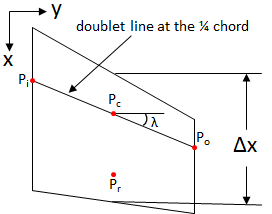
\includegraphics{DoubletLatticePanel.png}\hfill}
\begin{quote}\begin{description}
\item[{Attributes}] \leavevmode
\end{description}\end{quote}
\begin{itemize}
\item {} 
\emph{type (str)}: The type of object.

\item {} 
\emph{PANID (int)}: The integer ID linked with the panel.

\item {} 
\emph{xs (1x4 np.array{[}float{]})}: The x coordinates of the panel.

\item {} 
\emph{ys (1x4 np.array{[}float{]})}: The y coordinates of the panel.

\item {} 
\emph{zs (1x4 np.array{[}float{]})}: The z coordinates of the panel.

\item {} \begin{description}
\item[{\emph{DOF (dict{[}NID,factor{]})}: This dictionary is for connecting the movement}] \leavevmode
of the panel to the movement of an associated structure. Since a
panel's control point could be between two nodes (in the middle of an
element), the position of the panel can interpolated using a finite
element formulation. The NID's link the movement of the panel to the
movement of a corresponding node. The factor allows for a finite
element interpolation.

\end{description}

\item {} 
\emph{Area (float)}: The area of the panel.

\item {} 
\emph{sweep (float)}: The average sweep of the panel's doublet line.

\item {} 
\emph{delta\_x (float)}: The average chord line of the panel.

\item {} 
\emph{l (float)}: The length of the panel's doublet line.

\item {} 
\emph{dihedral (float)}: The dihedral of the panel.

\item {} 
\emph{Xr (1x3 np.array{[}float{]})}: The coordiantes of the panel's sending point.

\item {} \begin{description}
\item[{\emph{Xi (1x3 np.array{[}float{]})}: The coordinates of the panel's inboard}] \leavevmode
sending point.

\end{description}

\item {} \begin{description}
\item[{\emph{Xc (1x3 np.array{[}float{]})}: The coordinates of the panel's center}] \leavevmode
sending point.

\end{description}

\item {} \begin{description}
\item[{\emph{Xo (1x3 np.array{[}float{]})}: The coordinates of the panel's outboard}] \leavevmode
sending point.

\end{description}

\end{itemize}
\begin{quote}\begin{description}
\item[{Methods}] \leavevmode
\end{description}\end{quote}
\begin{itemize}
\item {} \begin{description}
\item[{\emph{x}: Provided the non-dimensional coordinates eta and xi which go from -1}] \leavevmode
to 1, this method returns corresponding the x coordinates.

\end{description}

\item {} \begin{description}
\item[{\emph{y}: Provided the non-dimensional coordinates eta and xi which go from -1}] \leavevmode
to 1, this method returns corresponding the y coordinates.

\end{description}

\item {} \begin{description}
\item[{\emph{z}: Provided the non-dimensional coordinates eta and xi which go from -1}] \leavevmode
to 1, this method returns corresponding the z coordinates.

\end{description}

\item {} \begin{description}
\item[{\emph{J}:Provided the non-dimensional coordinates eta and xi which go from -1}] \leavevmode
to 1, this method returns the jacobian matrix at that point. This
method is primarily used to fascilitate the calculation of the panels
area.

\end{description}

\item {} 
\emph{printSummary}: Prints a summary of the panel.

\end{itemize}

\begin{notice}{note}{Note:}
The ordering of the xs, ys, and zs arrays should be ordered in a
\end{notice}

finite element convention. The first point refers to the root trailing edge
point, followed by the tip trailling edge, then the tip leading edge, then
root leading edge.
\index{J() (AeroComBAT.Aerodynamics.CQUADA method)}

\begin{fulllineitems}
\phantomsection\label{aerodynamics:AeroComBAT.Aerodynamics.CQUADA.J}\pysiglinewithargsret{\bfcode{J}}{\emph{eta}, \emph{xi}}{}
Calculates the jacobian at a point in the element.

This method calculates the jacobian at a local point within the panel
provided the master coordinates eta and xi.
\begin{quote}\begin{description}
\item[{Args}] \leavevmode
\end{description}\end{quote}
\begin{itemize}
\item {} 
\emph{eta (float)}: The eta coordinate in the master coordinate domain.*

\item {} 
\emph{xi (float)}: The xi coordinate in the master coordinate domain.*

\end{itemize}
\begin{quote}\begin{description}
\item[{Returns}] \leavevmode
\end{description}\end{quote}
\begin{itemize}
\item {} \begin{description}
\item[{\emph{Jmat (3x3 np.array{[}float{]})}: The stress-resutlant transformation}] \leavevmode
array.

\end{description}

\end{itemize}

\begin{notice}{note}{Note:}
Xi and eta can both vary between -1 and 1 respectively.
\end{notice}

\end{fulllineitems}

\index{\_\_init\_\_() (AeroComBAT.Aerodynamics.CQUADA method)}

\begin{fulllineitems}
\phantomsection\label{aerodynamics:AeroComBAT.Aerodynamics.CQUADA.__init__}\pysiglinewithargsret{\bfcode{\_\_init\_\_}}{\emph{PANID}, \emph{xs}}{}
Initializes the panel.

This method initializes the panel, including generating many of the
geometric properties required for the doublet lattice method such as
Xr, Xi, etc.
\begin{quote}\begin{description}
\item[{Args}] \leavevmode
\end{description}\end{quote}
\begin{itemize}
\item {} 
\emph{PANID (int)}: The integer ID associated with the panel.

\item {} \begin{description}
\item[{\emph{xs (1x4 array{[}1x3 np.array{[}float{]}{]})}: The coordinates of the four}] \leavevmode
corner points of the elements.

\end{description}

\end{itemize}
\begin{quote}\begin{description}
\item[{Returns}] \leavevmode
\end{description}\end{quote}
\begin{itemize}
\item {} 
None

\end{itemize}

\end{fulllineitems}

\index{printSummary() (AeroComBAT.Aerodynamics.CQUADA method)}

\begin{fulllineitems}
\phantomsection\label{aerodynamics:AeroComBAT.Aerodynamics.CQUADA.printSummary}\pysiglinewithargsret{\bfcode{printSummary}}{}{}
A method for printing a summary of the CQUADA panel.

Prints out a tabulated information about the panel such as it's panel
ID, and the coordinates of it's four corner points.
\begin{quote}\begin{description}
\item[{Args}] \leavevmode
\end{description}\end{quote}
\begin{itemize}
\item {} 
None

\end{itemize}
\begin{quote}\begin{description}
\item[{Returns}] \leavevmode
\end{description}\end{quote}
\begin{itemize}
\item {} 
\emph{summary (str)}: The summary of the CQUADA attributes.

\end{itemize}

\end{fulllineitems}

\index{x() (AeroComBAT.Aerodynamics.CQUADA method)}

\begin{fulllineitems}
\phantomsection\label{aerodynamics:AeroComBAT.Aerodynamics.CQUADA.x}\pysiglinewithargsret{\bfcode{x}}{\emph{eta}, \emph{xi}}{}
Calculate the x-coordinate within the panel.

Calculates the x-coordinate on the panel provided the desired master
coordinates eta and xi.
\begin{quote}\begin{description}
\item[{Args}] \leavevmode
\end{description}\end{quote}
\begin{itemize}
\item {} 
\emph{eta (float)}: The eta coordinate in the master coordinate domain.*

\item {} 
\emph{xi (float)}: The xi coordinate in the master coordinate domain.*

\end{itemize}
\begin{quote}\begin{description}
\item[{Returns}] \leavevmode
\end{description}\end{quote}
\begin{itemize}
\item {} 
\emph{x (float)}: The x-coordinate within the element.

\end{itemize}

\begin{notice}{note}{Note:}
Xi and eta can both vary between -1 and 1 respectively.
\end{notice}

\end{fulllineitems}

\index{y() (AeroComBAT.Aerodynamics.CQUADA method)}

\begin{fulllineitems}
\phantomsection\label{aerodynamics:AeroComBAT.Aerodynamics.CQUADA.y}\pysiglinewithargsret{\bfcode{y}}{\emph{eta}, \emph{xi}}{}
Calculate the y-coordinate within the panel.

Calculates the y-coordinate on the panel provided the desired master
coordinates eta and xi.
\begin{quote}\begin{description}
\item[{Args}] \leavevmode
\end{description}\end{quote}
\begin{itemize}
\item {} 
\emph{eta (float)}: The eta coordinate in the master coordinate domain.*

\item {} 
\emph{xi (float)}: The xi coordinate in the master coordinate domain.*

\end{itemize}
\begin{quote}\begin{description}
\item[{Returns}] \leavevmode
\end{description}\end{quote}
\begin{itemize}
\item {} 
\emph{y (float)}: The y-coordinate within the element.

\end{itemize}

\begin{notice}{note}{Note:}
Xi and eta can both vary between -1 and 1 respectively.
\end{notice}

\end{fulllineitems}

\index{z() (AeroComBAT.Aerodynamics.CQUADA method)}

\begin{fulllineitems}
\phantomsection\label{aerodynamics:AeroComBAT.Aerodynamics.CQUADA.z}\pysiglinewithargsret{\bfcode{z}}{\emph{eta}, \emph{xi}}{}
Calculate the z-coordinate within the panel.

Calculates the z-coordinate on the panel provided the desired master
coordinates eta and xi.
\begin{quote}\begin{description}
\item[{Args}] \leavevmode
\end{description}\end{quote}
\begin{itemize}
\item {} 
\emph{eta (float)}: The eta coordinate in the master coordinate domain.*

\item {} 
\emph{xi (float)}: The xi coordinate in the master coordinate domain.*

\end{itemize}
\begin{quote}\begin{description}
\item[{Returns}] \leavevmode
\end{description}\end{quote}
\begin{itemize}
\item {} 
\emph{z (float)}: The z-coordinate within the element.

\end{itemize}

\begin{notice}{note}{Note:}
Xi and eta can both vary between -1 and 1 respectively.
\end{notice}

\end{fulllineitems}


\end{fulllineitems}



\subsection{CAERO1}
\label{aerodynamics:caero1}\index{CAERO1 (class in AeroComBAT.Aerodynamics)}

\begin{fulllineitems}
\phantomsection\label{aerodynamics:AeroComBAT.Aerodynamics.CAERO1}\pysiglinewithargsret{\strong{class }\code{AeroComBAT.Aerodynamics.}\bfcode{CAERO1}}{\emph{SID}, \emph{x1}, \emph{x2}, \emph{x3}, \emph{x4}, \emph{nspan}, \emph{nchord}, \emph{**kwargs}}{}
Represents an aerodynamic surface.

This CAERO1 object represents an aerodynamic lifting surface to be modeled
using the doublet-lattice method.
\begin{quote}\begin{description}
\item[{Attributes}] \leavevmode
\end{description}\end{quote}
\begin{itemize}
\item {} 
\emph{type (str)}: The type of object.

\item {} 
\emph{SID (int)}: The integer ID linked with the surface.

\item {} 
\emph{xs (1x4 np.array{[}float{]})}: The x coordinates of the panel.

\item {} 
\emph{ys (1x4 np.array{[}float{]})}: The y coordinates of the panel.

\item {} 
\emph{zs (1x4 np.array{[}float{]})}: The z coordinates of the panel.

\item {} \begin{description}
\item[{\emph{mesh ((NPAN+1)x(NPAN+1) np.array{[}int{]})}: The panel ID's in the relative}] \leavevmode
positions of their corresponding panels.

\end{description}

\item {} \begin{description}
\item[{\emph{xmesh ((NPAN+1)x(NPAN+1) np.array{[}float{]})}: The x-coordinates of the}] \leavevmode
lifting surface nodes.

\end{description}

\item {} \begin{description}
\item[{\emph{ymesh ((NPAN+1)x(NPAN+1) np.array{[}float{]})}: The y-coordinates of the}] \leavevmode
lifting surface nodes.

\end{description}

\item {} \begin{description}
\item[{\emph{zmesh ((NPAN+1)x(NPAN+1) np.array{[}float{]})}: The z-coordinates of the}] \leavevmode
lifting surface nodes.

\end{description}

\item {} \begin{description}
\item[{\emph{CQUADAs (dict{[}PANID, CQUADA{]})}: A dictionary mapping panel ID's to}] \leavevmode
CQUADA panel objects.

\end{description}

\end{itemize}
\begin{quote}\begin{description}
\item[{Methods}] \leavevmode
\end{description}\end{quote}
\begin{itemize}
\item {} \begin{description}
\item[{\emph{x}: Provided the non-dimensional coordinates eta and xi which go from -1}] \leavevmode
to 1, this method returns corresponding the x coordinates.

\end{description}

\item {} \begin{description}
\item[{\emph{y}: Provided the non-dimensional coordinates eta and xi which go from -1}] \leavevmode
to 1, this method returns corresponding the y coordinates.

\end{description}

\item {} \begin{description}
\item[{\emph{z}: Provided the non-dimensional coordinates eta and xi which go from -1}] \leavevmode
to 1, this method returns corresponding the z coordinates.

\end{description}

\item {} \begin{description}
\item[{\emph{plotLiftingSurface}: Plots the lifting surface in 3D space. Useful for}] \leavevmode
debugging purposes.

\end{description}

\item {} 
\emph{printSummary}: Prints a summary of the panel.

\end{itemize}

\begin{notice}{note}{Note:}
The ordering of the xs, ys, and zs arrays should be ordered in a
\end{notice}

finite element convention. The first point refers to the root leading edge
point, followed by the root trailling edge, then the tip trailing edge,
then tip leading edge.
\index{\_\_init\_\_() (AeroComBAT.Aerodynamics.CAERO1 method)}

\begin{fulllineitems}
\phantomsection\label{aerodynamics:AeroComBAT.Aerodynamics.CAERO1.__init__}\pysiglinewithargsret{\bfcode{\_\_init\_\_}}{\emph{SID}, \emph{x1}, \emph{x2}, \emph{x3}, \emph{x4}, \emph{nspan}, \emph{nchord}, \emph{**kwargs}}{}
Constructor for the CAERO1 lifting surface object.

Provided several geometric parameters, this method initializes and
discretizes a lifting surface using CQUADA panel objects.
\begin{quote}\begin{description}
\item[{Args}] \leavevmode
\end{description}\end{quote}
\begin{itemize}
\item {} 
\emph{SID (int)}: The integer ID for the surface.

\item {} 
\emph{x1 (1x3 np.array{[}float{]})}: The coordinate of the root leading edge.

\item {} 
\emph{x2 (1x3 np.array{[}float{]})}: The coordinate of the root trailing edge.

\item {} 
\emph{x3 (1x3 np.array{[}float{]})}: The coordinate of the tip trailing edge.

\item {} 
\emph{x4 (1x3 np.array{[}float{]})}: The coordinate of the tip leading edge.

\item {} 
\emph{nspan (int)}: The number of panels to run in the spanwise direction.

\item {} \begin{description}
\item[{\emph{nchord (int)}: The number of panels to run in the chordwise}] \leavevmode
direction.

\end{description}

\end{itemize}
\begin{quote}\begin{description}
\item[{Returns}] \leavevmode
\end{description}\end{quote}
\begin{itemize}
\item {} 
None

\end{itemize}

\end{fulllineitems}

\index{plotLiftingSurface() (AeroComBAT.Aerodynamics.CAERO1 method)}

\begin{fulllineitems}
\phantomsection\label{aerodynamics:AeroComBAT.Aerodynamics.CAERO1.plotLiftingSurface}\pysiglinewithargsret{\bfcode{plotLiftingSurface}}{\emph{**kwargs}}{}
Plots the lifting surface using the MayaVi environment.

This method plots the lifting surface using the MayaVi engine. It is
most useful for debugging models, allowing the user to verify that the
wing they thought they generated is actually what was generated.
\begin{quote}\begin{description}
\item[{Args}] \leavevmode
\end{description}\end{quote}
\begin{itemize}
\item {} 
\emph{figName (str)}: The name of the figure

\end{itemize}
\begin{quote}\begin{description}
\item[{Returns}] \leavevmode
\end{description}\end{quote}
\begin{itemize}
\item {} 
\emph{(figure)}: MayaVi Figure of the laminate.

\end{itemize}

\end{fulllineitems}

\index{printSummary() (AeroComBAT.Aerodynamics.CAERO1 method)}

\begin{fulllineitems}
\phantomsection\label{aerodynamics:AeroComBAT.Aerodynamics.CAERO1.printSummary}\pysiglinewithargsret{\bfcode{printSummary}}{}{}
A method for printing a summary of the CAERO1 element.

Prints out the surface ID, as well as the number of chordwise and
spanwise panels.
\begin{quote}\begin{description}
\item[{Args}] \leavevmode
\end{description}\end{quote}
\begin{itemize}
\item {} 
None

\end{itemize}
\begin{quote}\begin{description}
\item[{Returns}] \leavevmode
\end{description}\end{quote}
\begin{itemize}
\item {} 
\emph{summary (str)}: A summary of the CAERO1 surface attributes.

\end{itemize}

\end{fulllineitems}

\index{x() (AeroComBAT.Aerodynamics.CAERO1 method)}

\begin{fulllineitems}
\phantomsection\label{aerodynamics:AeroComBAT.Aerodynamics.CAERO1.x}\pysiglinewithargsret{\bfcode{x}}{\emph{eta}, \emph{xi}}{}
Calculate the x-coordinate within the lifting surface.

Calculates the x-coordinate within the lifting surface provided the
desired master coordinates eta and xi.
\begin{quote}\begin{description}
\item[{Args}] \leavevmode
\end{description}\end{quote}
\begin{itemize}
\item {} 
\emph{eta (float)}: The eta coordinate in the master coordinate domain.*

\item {} 
\emph{xi (float)}: The xi coordinate in the master coordinate domain.*

\end{itemize}
\begin{quote}\begin{description}
\item[{Returns}] \leavevmode
\end{description}\end{quote}
\begin{itemize}
\item {} 
\emph{x (float)}: The x-coordinate within the element.

\end{itemize}

\begin{notice}{note}{Note:}
Xi and eta can both vary between -1 and 1 respectively.
\end{notice}

\end{fulllineitems}

\index{y() (AeroComBAT.Aerodynamics.CAERO1 method)}

\begin{fulllineitems}
\phantomsection\label{aerodynamics:AeroComBAT.Aerodynamics.CAERO1.y}\pysiglinewithargsret{\bfcode{y}}{\emph{eta}, \emph{xi}}{}
Calculate the y-coordinate within the lifting surface.

Calculates the y-coordinate within the lifting surface provided the
desired master coordinates eta and xi.
\begin{quote}\begin{description}
\item[{Args}] \leavevmode
\end{description}\end{quote}
\begin{itemize}
\item {} 
\emph{eta (float)}: The eta coordinate in the master coordinate domain.*

\item {} 
\emph{xi (float)}: The xi coordinate in the master coordinate domain.*

\end{itemize}
\begin{quote}\begin{description}
\item[{Returns}] \leavevmode
\end{description}\end{quote}
\begin{itemize}
\item {} 
\emph{y (float)}: The y-coordinate within the element.

\end{itemize}

\begin{notice}{note}{Note:}
Xi and eta can both vary between -1 and 1 respectively.
\end{notice}

\end{fulllineitems}

\index{z() (AeroComBAT.Aerodynamics.CAERO1 method)}

\begin{fulllineitems}
\phantomsection\label{aerodynamics:AeroComBAT.Aerodynamics.CAERO1.z}\pysiglinewithargsret{\bfcode{z}}{\emph{eta}, \emph{xi}}{}
Calculate the z-coordinate within the lifting surface.

Calculates the z-coordinate within the lifting surface provided the
desired master coordinates eta and xi.
\begin{quote}\begin{description}
\item[{Args}] \leavevmode
\end{description}\end{quote}
\begin{itemize}
\item {} 
\emph{eta (float)}: The eta coordinate in the master coordinate domain.*

\item {} 
\emph{xi (float)}: The xi coordinate in the master coordinate domain.*

\end{itemize}
\begin{quote}\begin{description}
\item[{Returns}] \leavevmode
\end{description}\end{quote}
\begin{itemize}
\item {} 
\emph{z (float)}: The y-coordinate within the element.

\end{itemize}

\begin{notice}{note}{Note:}
Xi and eta can both vary between -1 and 1 respectively.
\end{notice}

\end{fulllineitems}


\end{fulllineitems}



\chapter{Indices and tables}
\label{index:indices-and-tables}\begin{itemize}
\item {} 
\DUspan{xref,std,std-ref}{genindex}

\item {} 
\DUspan{xref,std,std-ref}{modindex}

\item {} 
\DUspan{xref,std,std-ref}{search}

\end{itemize}


\renewcommand{\indexname}{Python Module Index}
\begin{theindex}
\def\bigletter#1{{\Large\sffamily#1}\nopagebreak\vspace{1mm}}
\bigletter{a}
\item {\texttt{AeroComBAT.Aerodynamics}}, \pageref{aerodynamics:module-AeroComBAT.Aerodynamics}
\item {\texttt{AeroComBAT.AircraftParts}}, \pageref{AircraftParts:module-AeroComBAT.AircraftParts}
\item {\texttt{AeroComBAT.FEM}}, \pageref{FEM:module-AeroComBAT.FEM}
\item {\texttt{AeroComBAT.Structures}}, \pageref{structures:module-AeroComBAT.Structures}
\end{theindex}

\renewcommand{\indexname}{Index}
\printindex
\end{document}
